\documentclass[12pt]{article}

\usepackage{graphicx}
\usepackage[margin=0.7in,footskip=0.2in]{geometry}%big footskip brings number down, small footskip brings number up
\usepackage{amsmath}
\usepackage{amssymb}
\usepackage[T1]{fontenc}
\usepackage{listings}
\usepackage{bm}
\usepackage{hyperref}
\usepackage{setspace}
\usepackage[usenames]{color}
\usepackage[utf8]{inputenc}
\usepackage{wrapfig}
\usepackage{relsize}
\usepackage{psfrag}
\usepackage{dsfont}
\usepackage{bbding}
\usepackage{caption}

\hypersetup{colorlinks   = true, %Colors links instead of ugly boxes
            urlcolor     = black, %Color for external hyperlinks
	    citecolor    = blue,
	    linkcolor    = black
}

\renewcommand*\contentsname{Table of Contents}

\newcommand{\E}[1]{
        \mathbb{E}\left[~#1~\right]
}

\def \oner {
	\mathlarger{\mathds{1}}
}

\newcommand{\argmin}{\operatornamewithlimits{argmin}}
\newcommand{\argmax}{\operatornamewithlimits{argmax}}
\newcommand*{\approxdist}{\mathrel{\vcenter{\offinterlineskip
\vskip-.25ex\hbox{\hskip.55ex$\cdot$}\vskip-.25ex\hbox{$\sim$}
\vskip-.5ex\hbox{\hskip.55ex$\cdot$}}}}
%\def\checkmark{\tikz\fill[scale=0.4](0,.35) -- (.25,0) -- (1,.7) -- (.25,.15) -- cycle;} 
%\DeclareMathOperator*{\argmax}{arg\,max}


\def \Eix {
	\mathbb{E}\left[~\text{I}(\bm{x})~\right]
}

\def \EIx {
	\mathbb{E}\left[~\text{I}(\underline{\bm{x}})~\right]
}

\def \Ix {
	\text{I}(\underline{\bm{x}})
}

\def \ix {
	\text{I}(\bm{x})
}

\def \roseLamb {
	0.5	
}

\def \rastLamb {
	0.4
}

\def \lockLamb {
	0.4
}

\begin{document}
% 
%
\title{Assessing Convergence in Gaussian Process Surrogate Model Optimization}
\author{Nicholas R. Grunloh and Herbert K. H. Lee}
\date{}
\maketitle
%
%

%
% \newgeometry{ margin=1in, top=0.70in, footskip=0.4in }
\begin{abstract}
%due to the subjective nature of convergence 
Identifying convergence in numerical optimization is an ever-present, difficult, and often subjective task. 
%, sequential design,
The statistical framework provided by Gaussian Process surrogate model optimization provides useful secondary measures for tracking optimization progress; however the identification of convergence via these criteria has often provided only limited success and often requires a more subjective analysis. % it these measures still subjective. % that can be used to identify convergence. 
%to track the expected improvement criterion to make
Here we use ideas originally introduced in the field of Statistical Process Control to define convergence in the context of an robust and objective convergence heuristic. 
% to remove this subjectivity from the identification of convergence.
The Exponentially Weighted Moving Average (EWMA) chart provides an ideal starting point for adaptation to track convergence via the EWMA convergence chart introduced here.
\\\\
{\bf \color{red}Keywords:} Convergence, Derivative-free Optimization, Emulator, Expected Improvement.
\end{abstract}
 
\doublespacing
%
%

%
%
\section{Introduction}
%
%

%% ______ a wide range of objective function applications.
%%notable {\color{red}In the absence of derivative information, numerical optimization} is a 
%%Derivative-free optimization's independence; optimization routine
%%In the world of derivative-free optimization; In the absence of derivative information derivative-free
%Releasing numerical optimization from its dependence on derivative information, has made black-box optimization a powerful and flexible tool for solving a wide range of engineering problems.
%%
%Of primary interest here, is the application of derivative-free optimization on computationally expensive black-box objective functions, such as computer simulations.
%%{\color{red}, in the real world}
%Often computer simulations can function as fast, cost-effective, development test beds for processes that are otherwise too expensive, or dangerous, to test physically. 
%% complex case study
%For example, the Lockwood pump-and-treat simulator, discussed in more detail in section {\color{red}XX}, computationally simulates the flow of contaminated ground-water alongside the Yellowstone River as numerical solutions to coupled systems {\color{red}cite}.
%%, as efficiently as possible control
%The focus of the Lockwood simulation is to optimize the management of this contaminated ground-water flow, so as to avoid contamination of the river.
%%control schemes
%However, the space of possible management schemes is large, and it is hard to identify when derivative-free optimization has converged to an optimal solution.
%%Due to the computational expense of such simulators, it is often desirable to optimize while evaluating the simulation as seldomly as possible, without sacrificing the quality of the solution.
%Due to the computational expense of such simulators, it is desirable to do effective optimization with as few simulation evaluations as possible.
%%This is achieved; The idea is to achieve this end
%This is achieved by efficiently exploring the solution space and limiting the number of function evaluations by robustly recognizing convergence.

%
%

%is an important problem with
Black-box derivative-free optimization has a
wide variety of applications, especially in the realm of computer
simulations \cite{KoldLewiTorc2003,gramacy2014}.  
%
When dealing with computationally expensive computer
models, a key question is that of convergence of the optimization.
%
Because each function evaluation is expensive, one wants to terminate
the optimization as early as possible.  
%
However for complex simulators, the response surface may be ill-behaved and optimization
routines can easily become trapped in a local mode, so one needs to
run the optimization sufficiently long to achieve a robust solution.
%
In this paper, we provide an automated method for assessing convergence of 
Gaussian Process surrogate model optimization by bringing in elements
of Statistical Process Control.

%
%

%
Our motivating example is a hydrology application, the Lockwood
pump-and-treat problem \cite{lockCite}, discussed in more detail in Section \ref{sec:lockwood}, wherein contamination in the ground-water near the
Yellowstone River is remediated via a set of treatment wells.  
%
The goal is to minimize the cost of running the wells while ensuring that
no contamination enters the river.  
%
The contamination constraint results in a complicated boundary that is unknown in advance and
requires evaluation of the simulator, and thus finding the global
constrained minimum is a difficult problem where it is easy for
optimization routines to, at least temporarily, get stuck in a local
minimum.  
%
Without knowing the answer in advance, how do we know when
to terminate the optimization routine?


%
%

%related to; is often employed for optimization of computer simulation experiments.
%, a relatively quick, statistical model of the objective function output; this model serves as surrogate of the objective function itself and .
The context of this paper is Gaussian Process surrogate model
optimization, a statistical modeling approach to derivative-free
numerical optimization that constructs a fast approximation to
the expensive computer simulation using a statistical surrogate model \cite{tgp2}.
%
%The surrogate model is relatively fast to work with, as compared with a large computer simulation, and 
Analysis of the surrogate model allows for efficient exploration the objective solution space.  
%
Typically a Gaussian Process (GP) surrogate model is chosen for its
robustness, relative ease of computation, and its predictive framework
\cite{santnerBook}.
%   landscape of the simulation parameters assessing future points of exploration on
Arising naturally from the GP predictive distribution \cite{gBook, EIPPD}, the maximum Expected Improvement (EI) criterion has shown to be a valuable criterion for guiding the exploration of the objective function and shows promise for use as a convergence criterion \cite{taddyOpt, jonesEIOpt}. %furthermore the EI shows promise for use as a convergence criterion {\color{red}cite}.
%The maximum Expected Improvement (EI) criterion has shown to be a valuable criterion, arising naturally from the GP predictive distribution {\color{red}cite}.
%
% The EI criterion can be used to assess future points of exploration on the objective function, as well as for monitoring the overall convergence of the optimization routine at large {\color{red}cite}.
% As such, the evaluation of the simulator is often the rate-limiting step for numerical optimization.


%
%

%however; as a means of assessing convergence GP surrogate
%{\color{red}Literature cite} recommends considering the EI as a convergence criterion for surrogate model optimization; as of yet, little work has been done to describe what convergence of these algorithms actually looks like in the context of the EI criterion.
Taddy et al. \cite{taddyOpt} considers the use of the improvement distribution for identifying global convergence; stating its value for use in applied optimization.
%, but it has not yet been established if there is some threshold EI value that is sufficient
The basic idea behind the use of improvement in identifying convergence is that convergence should occur when the surrogate model produces low expectations for discovering new optimum; that is to say, globally small EI values should be associated with convergence of the algorithm.
%claim that there exists 
Thus a simplistic stopping rule might first define some lower EI threshold, then claim convergence upon the first instance of an EI value falling below this threshold, as seen in \cite{windExample}.    
%in many different; of many other numerical optimization routines; that have been designed specifically to exhibit such behavior upon convergence  
This use of EI as a convergence criterion is analogous to other standard convergence identification methods in numerical optimization (e.g., the vanishing step sizes of a Newton-Raphson algorithm).
%
However, applying this same threshold strategy to the convergence of surrogate model optimization has not yet been adequately justified.
%, derived from the predictive distribution of the underling GP model; behavior
In fact, this use of EI ignores the nature of the EI criterion as a random variable, and oversimplifies the stochastic nature of convergence in this setting.
%
Thus it is no surprise that this treatment of the EI criterion can result in an inconsistent stopping rule as demonstrated in \mbox{Figure (\ref{introFig}).}  

\clearpage
%
%
\begin{figure}
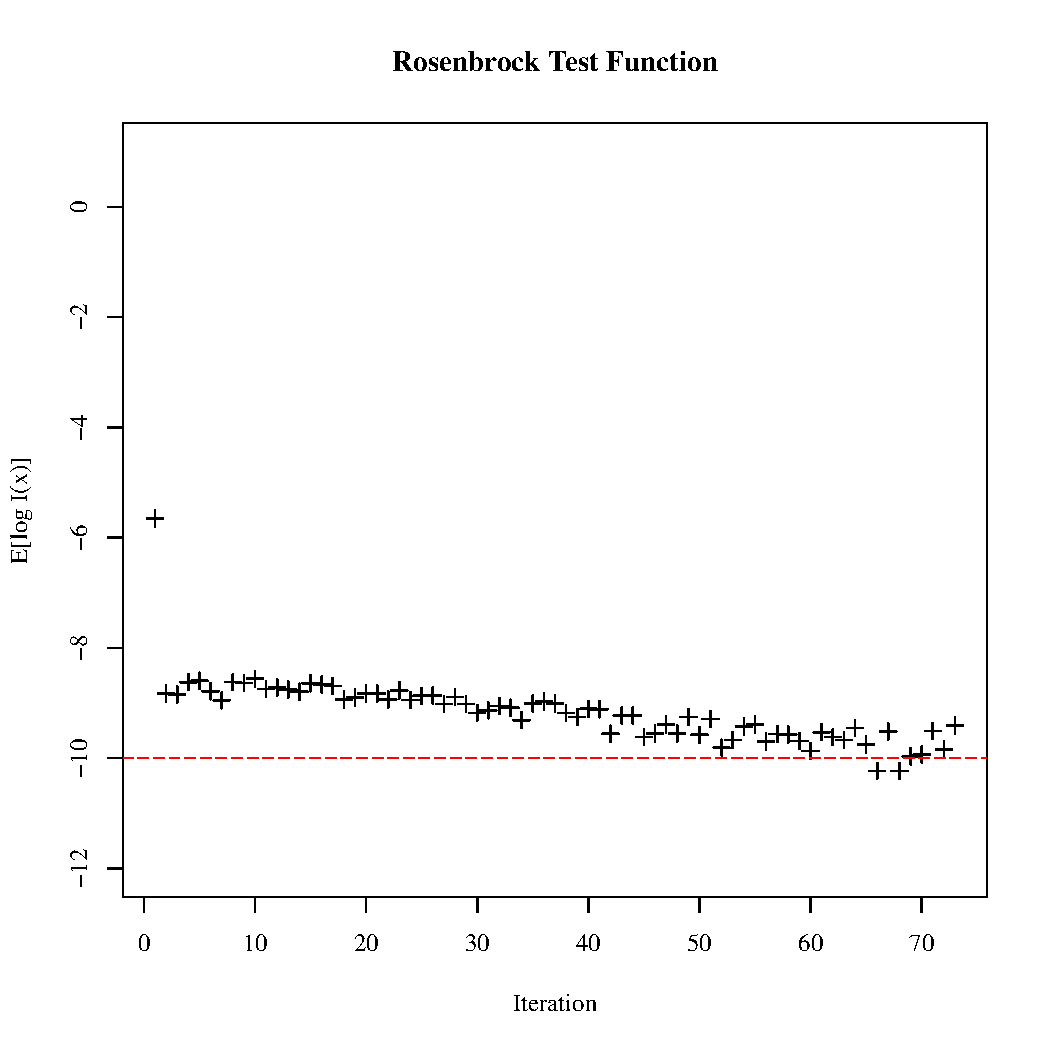
\includegraphics[width=0.32\textwidth]{./figures/introChartRoseEasyEasyAxis.pdf}
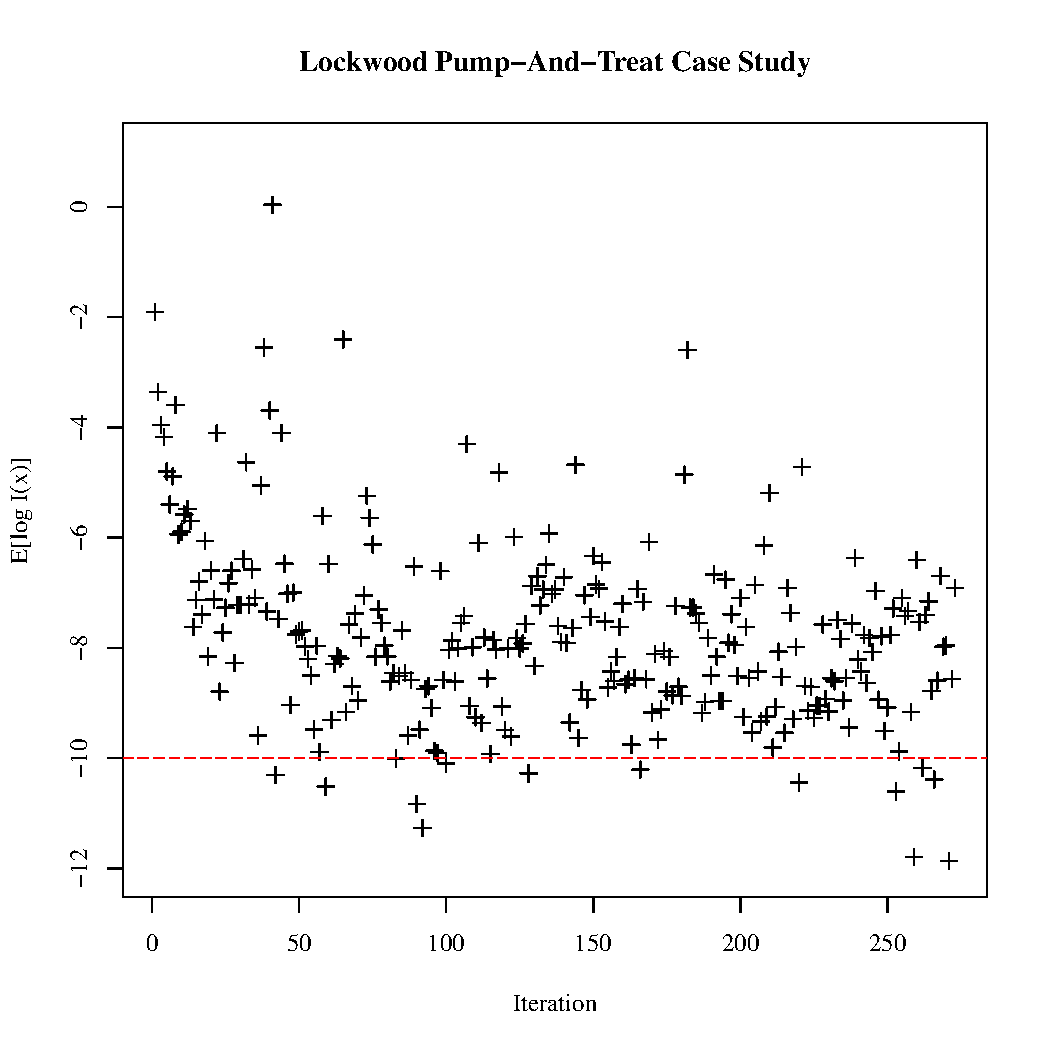
\includegraphics[width=0.32\textwidth]{./figures/introChartLock6Three20000Axis.pdf}
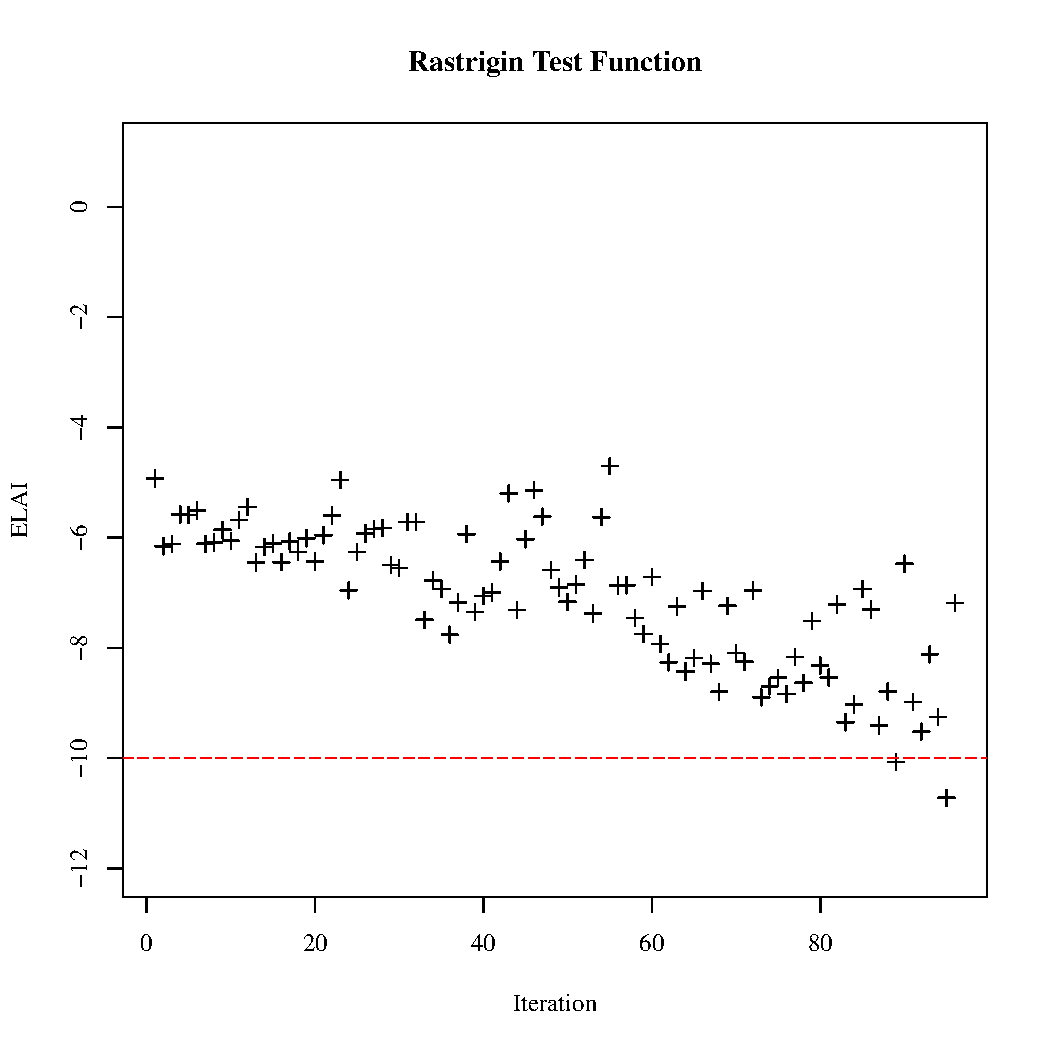
\includegraphics[width=0.32\textwidth]{./figures/introChartRastHardAxis.pdf}
\caption{
%
Three ELAI series (more details in Section~\ref{sec:examples}) plotted alongside an example convergence threshold value shown as a dashed line at -10.
}
\label{introFig}
\end{figure}
%
%

%of the series value; of the values; shows; non-negative
Because EI is strictly positive but decreasingly small,
we find it more productive to work on the log scale, using a lognormal
approximation to the improvement distribution to generate a more appropriate convergence criterion, as described in more
detail in Section~3.2.
%
Figure~(\ref{introFig}) represents three series of the Expected
Lognormal Approximation to the Improvement (ELAI) convergence criterion values from three
different optimization problems that will be demonstrated later in
this paper, where it will be shown that convergence is established near
the end of each of these series.
%as generated by 
These three series demonstrate various ELAI convergence behaviors, and
illustrate the difficulty in assessing convergence.  
%asymptotic properties of the; in more detail; improve
%In each panel the y-axis represents a monotone transformation of the basic EI criterion {\color{red}(i.e. ELI)} so as to benefit the asymptotic behavior of the improvement criterion's distribution, to be discussed further in Section {\color{red}XX}.
%
In the left-most panel, optimization of the Rosenbrock test function 
results in a well-behaved series of ELAI values, demonstrating a case in 
which the simple threshold stopping rule can accurately identify convergence.
%as this series
However the center panel (the Lockwood problem) demonstrates a failure of 
the threshold stopping rule, as this ELAI series contains much more 
variance, and thus small ELAI values are observed quite regularly.
%for the remainder of the series.
In the Lockwood example a simple threshold stopping rule could falsely
claim convergence within the first 50 iterations of the algorithm.
%
The large variability in ELAI with occasional large values indicates that 
the optimization routine sometimes briefly settles into a local minimum but is 
still exploring and is not yet convinced that it has found a global minimum.
%, additionally as the algorithm proceeds, several improvements of the objective function are discovered while ELI values repeatedly fall below the convergence threshold. %, all while the optimization routine continues to find several improved values of the objective function.
This optimization run appears to have converged only after the
larger ELAI values stop appearing and the variability has decreased.
%
Thus one might ask if a decrease in variability, or small variability,
is a necessary condition for convergence.  
%
The right-most panel (the Rastrigin test function) 
shows a case where convergence occurs by meeting the threshold level,
but where variability has increased, demonstrating that a decrease in
variability is not a necessary condition.

%
%

%
As the Improvement function is itself a random variable, attempting to 
set a lower threshold bound on the EI, without consideration of the underlying 
EI distribution over time, over-simplifies the dynamics of convergence
in this setting. 
%
Instead, we propose taking the perspective of Statistical
Process Control (SPC), where a stochastic series is monitored for 
consistency of the distribution of the most recently observed values.
In the next section, we review the statistical surrogate model approach and the use of EI for optimization.  In Section~\ref{sec:convergence}, we discuss our inspiration from SPC and how we construct our convergence chart.  Section~\ref{sec:examples} provides synthetic and real examples, and then we provide some conclusions in the final section.

%
%
\section{Gaussian Process Surrogate Model Optimization}
\label{sec:gp}
%
%

%
The primary motivation for the use of surrogate modeling in optimization is to manage a computationally challenging objective function with the use of a fast and relatively simple functional working model (i.e. the surrogate model) of the problem function. 
%
The surrogate model serves as an efficient tool for using function evaluations to infer the expected behavior of the objective function and thus determine where further optima may exist with minimal evaluation of the complex objective function itself.
%
Surrogate modeling is therefore useful for optimizing large computer simulations experiments, where each function evaluation may consume considerable computational resources, while the surrogate model can be evaluted quickly.
%
The standard surrogate model in the literature for analysis of computer experiments is a Gaussian Process (GP) \cite{sacksDesign, santnerBook}. A GP is a stochastic process such that when evaluated at any finite collection of points, that collection follows a multivariate Gaussian distribution. A GP is defined by its mean function and its covariance function, and various standard formulations exist \cite{abrahamsenBook,steinBook}. Most formulations take advantage of a large degree of smoothness, reflecting a modeling assumption of smoothness in the output of the simulator, in that if the simulator is evaluated at two nearby inputs, then one expects the resulting outputs to be relatively close. A GP can interpolate, which can be useful for a deterministic simulator, or it can smooth, which has a number of practical advantages even for deterministic simulators \cite{gramacy2012}.

%GP surrogate modeling considers the objective function $f \sim \text{GP}\big(m(\bm{x}), ~C(\bm{x}, \bm{x}')\big)$, and thus aims to minimize the number of actual function evaluations by using the GP predictive surface to interpolate between function evaluations.
%learning
%The surrogate can be used to minimize the number of evaluations by accurately interpolating between function evaluations and contributing information about where further evaluations of the objective function may be most useful for finding new optima.
%Considering the goals of surrogate modeling in optimization, 
% In particular, GP surrogate models have become a standard tool for analysis of computer emulation experiments .
%
% GP models 
%Inference on such GP models seems to strike an equitable balance between relative ease of computation and efficient learning of the true objective function behavior.
%
%making them ideal candidates for use as surrogate models here.

%
%

%
%As with most popular optimization strategies for optimizing functions over a real domain, GP surrogate optimization can make use of the assumption of some cohesive smoothness of the objective function.
%
%This smoothness relates points close in space, with similar expectations for the objective value, providing the primary mechanism by which optimization may proceed in most numerical algorithms. 
%
%GPs can directly express this assumption of smoothness with the a'priori choice of an appropriate covariance function which smoothly relates points through their relative positions in the domain.
%
%The choice of a covariance function to represent a smooth objective function is the typical modeling choice for optimization in computer emulation \cite{santnerBook}, although theoretically GPs may accommodate many common covariance structures \cite{abrahamsenBook, steinBook}. 
%s smoothness based upon the particular 
% to relate  models require that the of smooth objective functions on $\mathbb{R}^p$.
%

%
%

%
In many cases the assumption of a globally smooth $f$ with a homogeneous uncertainty structure can provide an effective and parsimonious model.
%smoothness in the GP covariance structure may make sense for a wide variety of objective functions, it is desirable to 
However for the sake of providing a flexible surrogate model, it is desirable to have the ability to loosen these restrictions in cases when $f$ may have inherently sharp boundaries, or when numerical simulators have variable stability in portions of the domain. 
%
Gramacy and Lee \cite{gpJasa} use the idea of allowing subpopulations of flexibility via a treed partitioning of the domain, fitting stationary GP surfaces to separate portions of $f$.
%
The domain is recursively sub-partitioned and separate hierarchically-linked GP models are fit within each sub-partition.
%
The partitioning scheme is fit via a reversible jump MCMC algorithm, jumping between models with differing partitioning schemes, and averaging over the full parameter space to provide smooth predictions except where the data call for a discontinuous prediction.
%
Partitioning the domain in this way allows parsimonious surrogate models in simple objective function cases and quite flexible surrogate models when the the objective function displays complex behavior. 
%
For further explanation of partitioned Gaussian process models as well as notes on implementing such models in R, see the R package \verb tgp  \cite{tgp, tgp2}.  Because many of the objective functions of interest are not well modeled by a stationary GP, we use treed GPs as our surrogate models in this paper, but our approach is easily adaptable to a wide variety of surrogate models.

% 	In many cases the assumption of a smooth $f$ with a homogeneous uncertainty structure can provide an effective and parsimonious model.
% 	%
% 	However for the sake of providing a flexible surrogate model, it is desirable to have the ability to loosen these restrictions in cases when $f$ looks more like the Grand Canyon, as opposed to the Great Plains.     
% 	%objective landscape
% 	Gramacy and Lee \cite{gpJasa} introduce the idea of allowing this flexibility via a treed partitioning of the domain.
% 	%
% 	This allows separately stationary GP surfaces to fit separately stationary portions of $f$.
% 	%
% 	For further explanation of partitioned Gaussian process models as well as notes on implementing such models in R, see the R package \verb tgp  \cite{tgp, tgp2}.

% surrogate models should compute in a relatively short amount of time as compared with the objective function quick to compute, and should quickly learn the behavior of the 
% 
% , based on the available data from the objective function. and thus aid use each evaluation of the objective function as a  
% It is of primary interest that the surrogate model can  efficiently incorporate each function evaluation 
% 
% %
% The primary idea behind surrogate modeling is to manage computationally difficult objective functions by constructing a functional working model (i.e. a surrogate model) of the true objective function, to be optimized, to represent as much about the objective function as our current data allows.
% %
% Surrogate modeling is a useful tool for application to large computationally expensive 
% %
% The primary role of surrogate modeling is to quickly and as accurately as possible construct a    optimization the primary 

%
%
% \begin{itemize}
% % \item {\color{red} *Everybody uses GP, bunch of cites}
% %
% % \item Gaussian process surrogate modeling has become a standard tool for analysis of computer emulation experiments \cite{sacksDesign, santnerBook} as well as many 
% %
% % \item other applications in which an a'priori assumption of smoothness is useful .
% %
% % \item For the sake of optimization, the assertion of a smooth objective function, $f$, serves as the basis for most efficient searching algorithms.%, as is explicitly the case with GP.
% %
% % \item In the case of GP surrogate modeling, the Gaussian Process theory can explicitly express this desire for smoothness through the a'priori choice of a covariance function with the desired smoothness properties.
% %
% % \item Although smoothness is key to search, and 
% %  
% \item For the sake of optimization practically all opt we only have a hope of efficiently searching $f$ if we assume that $f$ provides a reasonably smooth, otherwise optimization by any method is practically infeasible.
% %
% \item However it is not 
% 
% %
% \item \cite{gpJasa, tgp, tgp2}
% %
% \item {\color{red} *Expand Treed Partitioning}
% %
% \item For additional modeling details, including loosening the assumption of global stationarity, and details about implementing GP models in the context of numerical optimization see the R package \verb tgp ~as well as the associated vignettes \cite{tgp, tgp2}.
% \end{itemize}


% If we have any hope of finding optima of a function, $f$, we impose the condition that $f$ provides a reasonably smooth mapping for relating points in the domain, $\bm{x}$, to response values, $z(\bm{x})$.
% optimization of functions over $\mathbb{R}^p$
% %
% GP surrogates, as with many optimization strategies for objective function on $\mathbb{R}^p$, rely upon some sense of cohesive smoothness of the objective function, which relates points close in space with similar expectations for the objective value.

% {\color{red} *Everybody uses GP, bunch of cites}
% 
% %
% For more details on the theoretical foundations of Gaussian Processes in computer experiments see \cite{santnerBook}.
% %
% If we have any hope of finding optima of a function, $f$, we impose the condition that $f$ provides a reasonably smooth mapping for relating points in the domain, $\bm{x}$, to response values, $z(\bm{x})$.
% %\text{\textbf{Z}}; $\big($i.e.~\big)$; \text{Z}
% The $z(\bm{x})$ are assumed to be particular realizations of an infinitely dimensional generalization of the multivariate normal distribution, $f \sim \text{GP}(m,~K)$, and thus jointly any set of such realizations, $z(\bm{x})$, jointly follow a multivariate normal distribution.
% %
% As part of the GP model specification, we specify the mean function as a linear combination of simple basis functions, $m=\bm{\beta}^\intercal \text{\textbf{f($\bm{x}
% $)}}$, and we describe the covariance structure, among the dimensions of the $z(\bm{x})$, through specification of a covariance function, $K(\bm{x}, \bm{x}')$.
% %
% By specifying a homogeneous covariance function, we thus model the relationship between $||\bm{x}-\bm{x}'||$ with the correlation structure that we expect to see when jointly considering two such realizations of the GP. 
% %
% The following exponential power family provides an example of a reasonable choice of $K(\bm{x}, \bm{x}')$, under the assumption of a reasonably well behaved $f$,
% %
% \begin{equation}
% K(\bm{x}, ~\bm{x}') = \sigma^2\exp\left\{ -\frac{||\bm{x}-\bm{x}'||^p}{d} \right\}.
% \label{corrFunc}
% \end{equation} 
% %
% Specifying conjugate priors for $\bm{\beta}$ and $\sigma^2$ yields a straightforward Gibbs sampling posterior inferential setting with the exception of the covariance structure parameters requiring Metropolis-Hastings MCMC sampling.


%
%
\subsection{Expected Improvement}
%
%

%
%The EI criterion has been used \cite{tgp2}, \cite{taddyOpt} to identify candidate points that have a strong {\it possibility of encountering new minima}.
%when applied to a single candidate point has
The EI criterion predicts how likely it will be to find a new minimum at a given location based on the predictive surrogate model.  EI is built upon the improvement function \cite{jonesEIOpt}:
%
%The improvement function takes the following form,
\begin{equation}
\ix~=~ \max \Big\{ \big(f_{min} - f(\bm{x})\big), ~0 \Big\},
\label{ix}
\end{equation}
%
where $f_{min}$ is the smallest function value observed so far.  EI is the expectation of the improvement function with respect to the posterior predictive distribution of the surrogate model, $\Eix$.
EI rewards candidates both for having a low predictive mean, as well high uncertainty (where the function has not been sufficiently explored).
%
By definition the improvement function is always non-negative, and the GP posterior predictive $\Eix$ is strictly positive.
%
EI is available in closed form for a stationary GP, and for other models can be quickly estimated using Monte Carlo posterior predictive samples at given candidate locations.

%
%
\subsection{Optimization Procedure}
%
%

%
%
\begin{wrapfigure}{r}{0.5\textwidth}
	\vspace{-1.6cm}
% 	\vspace{-2.5cm}
	\singlespacing
	\caption{Optimization Procedure}
	\begin{itemize}
	\item[1)] Collect an initial set, $\bm{X}$.
	\item[2)] Compute $f(\bm{X})$.
	\item[3)] Fit surrogate based on evaluations of $f$.
	\item[4)] Collect a candidate set, $\tilde{\bm{X}}$.
	%\item[5)] Compute $\Eix$ among $\tilde{\bm{X}}$.$\E{\text{I}(\tilde{\bm{x}_i}})$
	\item[5)] Compute EI among $\tilde{\bm{X}}$
	%\item[6)] Add $\tilde{\bm{x}_i}$ yielding largest $\Eix$ to $\bm{X}$.
	\item[6)] Add $\argmax_{\tilde{\bm{x}_i}} \E{\text{I}(\tilde{\bm{x}_i})}$ to $\bm{X}$.
	\item[7)] Check convergence.
	\item[8)] If converged exit. Otherwise go to 2).
	\end{itemize}
	\doublespacing
	%\vspace{-0.85cm}
	\label{procedure}
\end{wrapfigure}
%
%

% us with a
Optimization can be viewed as a sequential design process, where locations are selected for evaluation on the basis of how likely they are to decrease the objective funciton, i.e., based on the EI.
%The idea for optimization, in this context, is to only evaluate the objective function at locations that have a good chance of providing a new minimum. 
%I need a handle
Optimization begins by initially collecting a set, $\bm{X}$, of locations to evaluate the true function, $f$, to gather a basic impression of $f$.
% (\ref{gpModel})
A statistical surrogate model is then fitted with $f(\bm{X})$ as observations of the true function.
%EI randomly
Using the surrogate model, a set of candidate points, $\tilde{\bm{X}}$, are selected from the domain and the EI criterion is calculated among these points.
%
The candidate point that has the highest EI is then chosen as the best candidate for a new minimum and thus, it is added to $\bm{X}$.
% (\ref{gpModel})
The objective function is evaluated at this new location and the surrogate model is refit based on the updated $f(\bm{X})$.
%
The optimization procedure carries on in this way until convergence.  The key contribution of this paper is an automated method for checking convergence, which we develop in the next section. 

%
%
\section{EWMA Convergence Chart}
\label{sec:convergence}
%
%

%
%
\subsection{Statistical Process Control}
%
%

%
In Shewhart's seminal book \cite{shewhartBook} on the topic of control in manufacturing, Shewhart explains that a phenomenon is said to be in control when, ``through the use of past experience, we can predict, at least within limits, how the phenomenon may be expected to vary in the future.''
%, accounting not only for the the expected variability  not only consider particular values of the EI criterion, but it ( expected center, spread, and )
This notion provides an instructive framework for thinking about convergence because it offers a natural way to consider the distributional characteristics of the EI as a proper random variable. 
% of that statistic.
In its most simplified form, SPC considers an approximation of a statistic's sampling distribution as repeated sampling occurs in time.
Thus Shewhart can express his idea of control as the expected behavior of random observations from this sampling distribution.
% from some data generating mechanism,
For example, an $\bar x$-chart tracks the mean of repeated samples (all of size $n$) through time so as to expect the arrival of each subsequent mean in accordance with the known or estimated sampling distribution for the mean, $\bar{x}_j \sim N\left(\mu, \frac{\sigma^2}{n}\right)$.   
%
%Shewhart expresses his idea of control as the expected behavior of random observations from the sampling distribution of interest.
%
By considering confidence intervals on this sampling distribution we can easily draw explicit boundaries (i.e., control limits) to identify when the process is in control and when it is not.
%
Observations violating our expectations (falling outside of the control limits) indicate an out-of-control state.
%
Since neither $\mu$ nor $\sigma^2$ are typically known, it is of primary importance to use the data carefully to form accurate approximations of these values, thus establishing a standard for control.
%
Furthermore, this logic relies upon the typical asymptotic results of the central limit theorem (CLT), and care should be taken to verify the relevant assumptions required.


It is important to note that we are not performing traditional SPC in this context, the EI criterion will be stochastically decreasing as an optimization routine proceeds.  Only when convergence is reached will the EI series look approximately like an in-control process.  Thus our perspective is completely reversed from the traditional SPC approach---we start with a process that is out of control, and we determine convergence when the process stabilizes and becomes locally in control.  An alternative way to think about our approach is to consider performing SPC backwards in time on our EI series.  Starting from the most recent EI observations and looking back, we declare convergence if the process starts in control and then becomes out of control.  This pattern generally appears only when the optimization has progressed and reached a local mode.  If the optimization were still proceeding, then the EI would still be decreasing and the final section would not appear in control.

%
%
\subsection{Expected Lognormal Approximation to the Improvement (ELAI)}
%
%

%
For the sake of obtaining a robust convergence criterion to track via SPC, it is important to carefully consider properties of the improvement distributions which generate the EI values.
%
% Ultimately, the distribution of the EI is asymptotically normal, but the characteristics of the improvement distribution, as convergence approaches, complicate these asymtoptics. 
%
The improvement criterion is strictly positive but decreasingly small, thus the improvement distribution is often strongly right skewed, and the EI is far from normal.
%
Additionally, this right skew becomes exaggerated as convergence approaches, due to the decreasing trend in the EI criterion.
%% distribution will always struggle to capture the resulting EI distribution.
Together these characteristics of the improvement distribution give the EI criterion inconsistent behavior for tracking convergence via a typical $\bar x$-chart. 
 
%
%

%log improvement
These issues naturally suggest releasing the bound at 0 by modeling transformations of the improvement, rather than directly considering the improvement distribution on its own.
%
One of the simplest of the many possible helpful transformations in this case would consider the log of the improvement distribution. 
%
However due to the MCMC sample-based implementation of the Gaussian Process, and the desire for a large number of samples from the improvement distribution, it is not uncommon to obtain at least one sample that is computationally indistinguishable from 0 in double precision.
%
Thus simply taking the log of the improvement samples can result in numerical failure, particularly as convergence approaches, even though the quantities are theoretically strictly positive.
%
Despite this numerical inconvenience, the distribution of the improvement samples is often very well approximated by the Lognormal distribution. 

%
%

%
We avoid the numerical issues by using a model-based approximation. With the desire to model $\mathbb{E}\left[~\log\text{I}~\right] \approxdist N\left(\mu, \frac{\sigma^2}{n}\right)$, we switch to a Lognormal perspecive.   
%
Recall that if a random variable \mbox{$X\sim Log$-$N(\psi, \nu)$,} then another random variable $Y=\log(X)$ is distributed $Y\sim N(\psi, \nu)$.
%{\color{red}cite}
Furthermore, if $m$ and $v$ are, respectively, the mean and variance of a lognormal sample, then the mean, $\psi$, and variance, $\nu$, of the associated normal distribution are given by the following relation.
%
\begin{eqnarray}
\psi = \log\left( \frac{m^2}{\sqrt{v+m^2}} \right) &~&  \nu = \log\bigg( 1+ \frac{v}{m^2} \bigg).
\label{lnRelate}
\end{eqnarray}
%
Using this relation we do not need to transform any of the improvement samples.
%
We compute the empirical mean and variance of the unaltered, approximately lognormal, improvement samples, then use relation (\ref{lnRelate}) to directly compute $\psi$ as the Expectation under the Lognormal Approximation to the Improvement (ELAI).
%Considering that the log improvement has reduced right skew, for the sake of improved asymptotics of the; of the $\E{\log\text{I}}$ distribution enjoys improved asymptotics
The ELAI convergence criterion is a useful convergence criterion in this case because of the reduced right skew of the log of the improvement distribution, and the ELAI convergence criterion serves as a computationally robust approximation of the $\E{\log\text{I}}$ under reasonable log-normality of the improvements.
%approximately
Furthermore, both the $\E{\log\text{I}}$ and ELAI convergence criterion are distributed approximately normally in repeated sampling.
%
This construction allows for more consistent and accurate use of the fundamental theory on which our SPC perspective depends.

%improvement provides robust asymptotics for the normality of the distribution of the $\E{\log\text{I}}$, even as convergence approaches the ELAI provides a good approximation for this value.
%{\color{red} ELAI}
% The ELAI provides a good approximation for 

%
%
\subsection{Exponentially Weighted Moving Average}
%
%

%
The Exponentially Weighted Moving Average (EWMA) control chart \cite{ewmaPaper, qccPack} elaborates on Shewhart's original notion of control by viewing the repeated sampling process in the context of a moving average smoothing of series data. %, rather than assuming a constant long run average, as in the $\bar x$-chart.    
%Principally provide particularly robust solutions to be expected for convergence in this setting.
Pre-convergence ELAI evaluations tend to be variable and overall decreasing, and so do not necessarily share distributional consistency among all observed values.  
%
Thus a weighted series perspective was chosen to follow the moving average of the most recent ELAI observations while still smoothing with some memory of older evaluations.
%stochastically slides into convergence, a series perspective is appropriate here; in particular the EWMA perspective has shown to be well suited for tracking the progression of means that are subject to subtle drifting processes \cite{adaptEWMA, ?}. %, just as displayed by the ELAI criterion upon convergence.
%
EWMA achieves this robust smoothing behavior, relative to shifting means, by assigning exponentially decreasing weights to successive points in a rolling average among all of the points of the series, thus the EWMA emphasizes recent observations and shifts the focus of the moving average to the most recent information while still providing shrinkage towards the global mean of the series.

%
%

%
If $Y_i$ is the current ELAI value, and $Z_i$ is the EWMA statistic associated with this current value, then the initial value $Z_0$ is set to $Y_0$ and for $i>0$ the EWMA statistic is expressed as,
%
\begin{equation}
Z_i=\lambda Y_i+(1-\lambda)Z_{i-1}.
\label{ewmaStat}
\end{equation}
%
Above, $\lambda$ is a smoothing parameter that defines the weight $\left( \text{i.e. }0<\lambda\le1\right)$ assigned to the most 
%
%
\begin{wrapfigure}{r}{0.41\textwidth}
\vspace{-0.8cm}
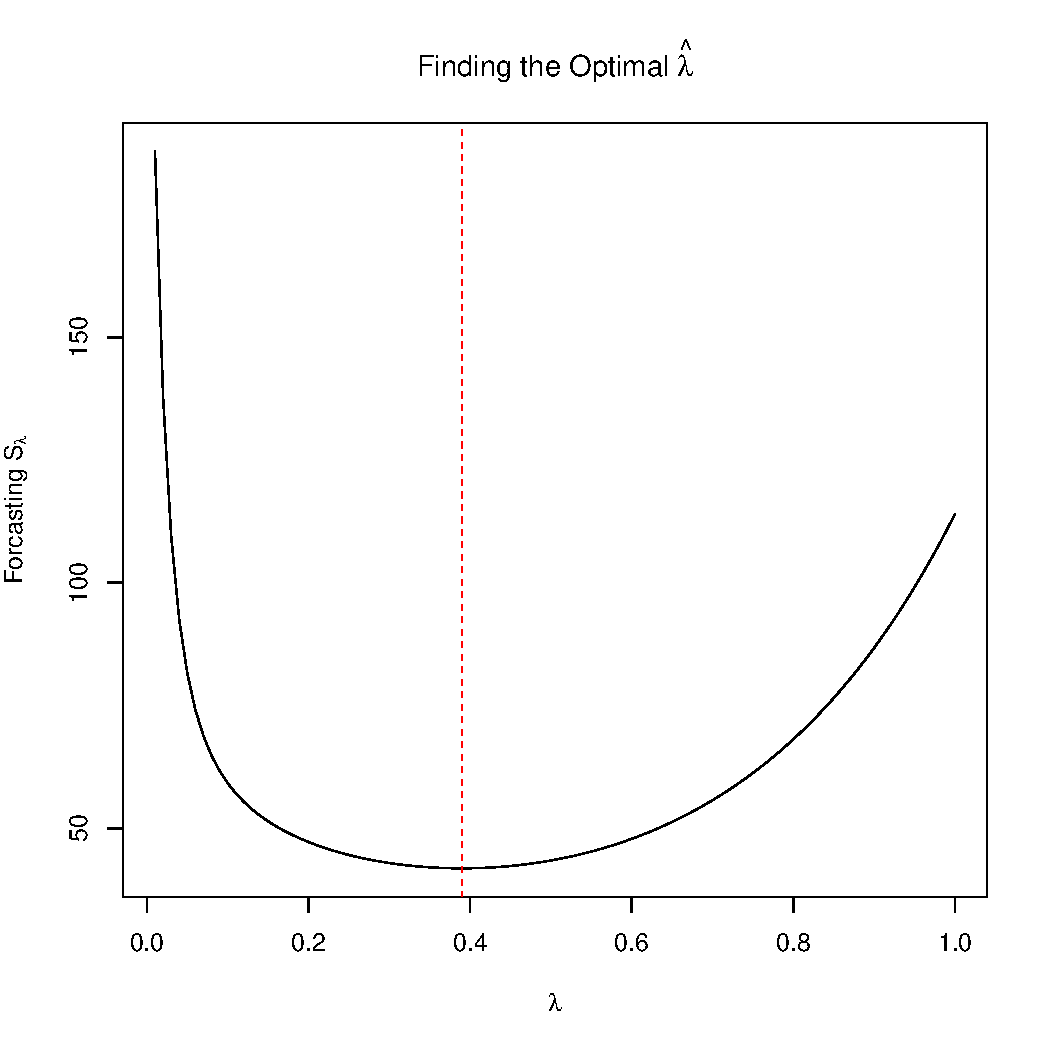
\includegraphics[width=0.4\textwidth]{./figures/ssRastHardOpt.pdf}
\caption{ $S_\lambda$ as calculated over a fine grid of possible $\lambda$ values for ELAI values derived from optimization of the Rastrigin test function. The optimal forecasting $\hat\lambda$ is shown by the vertical dashed line. }
\label{bestL}
\end{wrapfigure}
%
%
recent observation, $Y_i$.
%Eq. (\ref{ewmaStat})
The recursive expression of the statistic ensures that all subsequent weights geometrically decrease as they move back through the series.

%
Typical values of $\lambda$ can range from \mbox{$0.1\le\lambda\le0.3$}, with a default value of $\lambda$ around $0.2$, as described by Box et al. \cite{boxBook}.
%
Large values of $\lambda$ assign more weight to recent observations in the series, allowing for a more flexible fit for unstable series.
%
However, the choice of a large $\lambda$ may over-fit the $Z_i$ to noise in the $Y_i$.
%
It is thus desirable to choose to the smallest $\lambda$ which still provides good forecasts of future
observations in the series.
%
Box et al. \cite[p. 87]{boxBook} explains how to choose an optimal value for $\lambda$ by choosing the $\hat\lambda$ which minimizes the sum of squared forecasting deviations ($S_\lambda$) for each new observation.
%curvature
Through this analysis of $S_\lambda$, as seen in Figure~(\ref{bestL}), is it evident that EWMA charts can be very robust to reasonable choices of $\lambda$, due to the small first and second derivatives of $S_\lambda$ for a large range of sub-optimal choices of $\lambda$ around $\hat\lambda$. % as seen in Figure~(\ref{bestL}).
%
In fact, Figure~(\ref{bestL}) shows that for \mbox{$\lambda\in[0.2, 0.6]$,} $S_\lambda$ stays within 10\% of its the minimum possible value.

%
%

%
It is interesting to note that for the example series used in Figure~(\ref{bestL}), the optimal $\hat \lambda\approx$\rastLamb exceeds the recommended upper limit of 0.3 for $\lambda$. 
%
Discrepancies between the optimal values of $\lambda$ chosen here, and the typically chosen values of $\lambda$ can be naturally attributed to the differing context in which we apply EWMA as compared to the typical SPC application. 
%which obviously falls outside of the standard values for $\lambda$ mentioned above.
%would begin with starts
The typical use of EWMA in SPC begins with the premise of a relatively stable (in-control) series and attempts to identify new out-of-control observations which would indicate some change in the data generating process.
%
However our use of EWMA, to identify convergence, begins with an out-of-control series and we wish to identify when the series falls into control (i.e. convergence).
%
As a result, ELAI values for tracking convergence are inherently less stable than typical SPC applications of EWMA.
%% in the context of identifying convergence.
Due to the decreased stability of the series, in this context, the optimal forecasting $\hat\lambda$ may often fall above the traditionally recommended upper limit for $\lambda$, in-order to better follow the more active moving averages inherent to the unstable pre-convergence series. 
%
In this context we want to reiterate that while it is useful to borrow the EWMA machinery often used in SPC, we are approaching the whole process backwards, in that we are starting with an ``out of control'' process and waiting to see when it settles down into control, and thus our approach should be viewed as SPC-inspired rather than a formal application of SPC.
% but the ultimate analysis of the data should not explicitly be considered SPC, as the perspective of the data does not fully align with that of SPC.

%
%

%
Identifying convergence relies upon carefully defining the control limits on the EWMA statistic.
%
As in the simplified $\bar x$-chart, defining the control limits for the EWMA setting amounts to considering an interval on the sampling distribution of interest.
%, under the assumptions that the $Y_i$ arrive as $i.i.d.$ samples
In the EWMA case we are interested in the sampling distribution of the $Z_i$.
%, Lucas and Saccucci \cite{ewmaPaper}  show,
Assuming that the $Y_i$ are $i.i.d.$ then Lucas and Saccucci \cite{ewmaPaper} show that we can write $\sigma^2_{Z_i}$ in terms of $\sigma^2_{Y}$. 
%
\begin{equation}
\sigma^2_{Z_i} = \sigma^2_{Y}\left(\frac{\lambda}{2-\lambda}\right)\left[1-(1-\lambda)^{2i}\right]
\end{equation}
%\substack{i.i.d.\\\sim}
Thus if $Y_i \stackrel{i.i.d.}{\sim} N\left(\mu, \frac{\sigma^2}{n}\right)$, then the sampling distribution for $Z_i$ is $Z_i \sim N\left(\mu, \sigma^2_{Z_i}\right)$.
%
Furthermore by choosing a confidence level through choice of a constant $c$, the control limits based on this sampling distribution are seen in Eq. (\ref{EWMACL}).% follow on the next page.
%
%
%
\begin{equation}
\text{CL}_i = \mu \pm c \sigma_{Z_i}
=  \mu \pm c ~ \frac{\sigma}{\sqrt{n}}~\sqrt{\left(\frac{\lambda}{2-\lambda}\right)\left[1-(1-\lambda)^{2i}\right]}
\label{EWMACL}
\end{equation}
%
%

%
Notice that since $\sigma^2_{Z_i}$ has a dependence on $i$, the control limits do as well.
%the focusing effect of EWMA. % this focusing effect.\frac{\sigma}{\sqrt{n}}~
Looking back through the series brings us away from the focus of the moving average, at $i$, and thus the control limits widen until the limiting case as, $i\rightarrow\infty$, the control limits are defined by $\mu \pm c ~ \sqrt{\frac{\lambda\sigma^2}{(2-\lambda)n}}$.
%traversing backwards through the series resulting directly from the geometrically decreasing weights.

%
At first glance it is not clear that the $Y_i$ are in fact $i.i.d.$
%
Indeed the early iterations of the convergence processes seen in Figure (\ref{introFig}) certainly do not display $i.i.d.$ $Y_i$. 
%
However as the series approaches convergence, the $Y_i$ eventually do enter a state of control see Figure (\ref{ewmaFig}).
%
For these controlled $Y_i$ an $i.i.d.$ approximation is quite reasonable.
%
The realization of such a controlled region of the series defines the notion of consistency which is what allows for the identification of convergence. 

%
%
\subsection{The Control Window}
%
%

% for accurate identification of convergence is the introduction of a so called
%the distributional consistency we use to identify convergence
% that is necessary
The final structural feature of the EWMA convergence chart for identifying convergence is the so called {\it control window}.
%is a window containing
The control window contains a fixed number, $w$, of the most recently observed $Y_i$.
%The idea being, o
Only information from the $w$ points currently residing inside the control window is used to calculate the control limits, but the EWMA statistic is still computed for all $Y_i$ values.
%
Initially, the convergence algorithm is allowed to fill the control window, by collecting an initial set of $w$ observations of the $Y_i$.
%
As new observations arrive, the oldest $Y_i$ value is removed from the control window, thus allowing for the inclusion of a new $Y_i$.

%
%

%
The purpose of the control window is two-fold.
% examination
Firstly it serves to dichotomizes the series for evaluating subsets of the $Y_i$ for distributional consistency.
% convergence
Secondly it offers a structural way for basing the standard for consistency (i.e. the control limits) only on the most recent and relevant information in the series. 
%
%It is important to draw 
%This is important due to the subtle way in which ELAI values slide to convergence.

%
%

% {\color{red}
% %The size of this window is left up to the discretion of user,.
% The size, $w$, of the control window is an important parameter for correctly identifying convergence.
%
The size of the control window, $w$, may vary from problem to problem based on the difficulty of optimization in each case. %; ultimatly the choice of $w$ is left as tuning parameter of the system.
%
A reasonable way of choosing $w$ is to consider the number of observations neccissary to establish a standard of control. % with respect to the objective function at hand.
%
The choice of $w$ will naturally increase as the difficulty of the optimization problem increases.
%
%For example, if the objective function is in many dimensions, the choice of $w$ will neccisarily increase to allow the surrogate model to gather a proportional amount of information about $f$.  
%
%The choice of a conservativly large $w$ consistently provides a better identification of convergence, with large $w$ representing idealistic large sample sizes, and small $w$ correctly identifying convergence well only for well-behaved functions, with small search domains.
%the size of the control window may lead to premature identification of convergence, however if $w$ is too large, we compute 
%as $w$ may be veiwed in the context of 
%However, j(i.e. the cost of overadditional sampling)
Just as in other sample size calculations, the the choice of an optimal $w$ must consider the cost of premature identification of convergence (i.e. poor inference) associated with underestimating $w$, against the cost of continuing to sample after convergence has occurred (i.e. the cost of over sampling) associated with overestimating $w$.
%
Providing a default choice of $w$ is somewhat arbitrary without careful analysis of the particulars of the objective function behavior and the costs of each successive objective function evalutation, however as a recommendation for starting this analysis, one may consider $w\ge15p$ as a rule of thumb.
%
This recommendation considers the dimensionality, $p$, of the objective function as well as represents the prior assertion that premature identification of convergence is a worse error than computing extraneous objective function evaluations. 

%
%
%however the goal of identifying convergence is to 
%
% Choosing the correct value of $w$ presents an interesting decision problem since underestimating the size of the control window may lead to premature identification of convergence, however if $w$ is too large, we compute unnecessary objective function evaluations.
%
%

%
For example, if the objective function must be searched over a large domain, particularly in many dimensions, optimization will naturally take many function evaluations to gather adequate information to reflect confident identification of convergence.
%
Thus the EI criterion, and by extension the ELAI criterion, may display high variance, associated with high uncertainty, as well as be slow to decrease in mean value from the initial state of preconvergence into convergence.
%
Jointly the high ELAI variance and the slow decreasing mean value of the ELAI criterion may make it hard to identify convergence; in these cases large values of $w$ are required to discern this relatively slight signal in the context of increased noise.
%
Similar effects may be observed for highly multimodal objective functions, as the regular discovery of new modes will increase the variance of the ELAI criterion, and disguise any decreasing mean value, among the noise inherent to the search of such functions.

%
%
% %adequate algorithm willay EI criterion may commonly be slow to learn the  decrease from  display a large variance amoung amoung function evalutations, 
% % Because $w$ may vary from problem to problem it is ultimately left as a tuning parameter of the system.
% %
% 
% %
% As a general trend, {\color{blue}harder} optimization problems require larger values of $w$ since the EI criterion follows a less structured decreasing pattern as new modes are discovered at irregular patterns.
%
%

%
By contrast, strongly unimodal functions will enjoy a relatively fast decrease in the ELAI criterion in the presence of relatively small variability.
%
This higher signal-to-noise ratio makes for easier identification of convergence, and thus allows for a smaller choice of $w$. % to notice a move of the ELAI criterion into convergence.
%
However if $w$ is chosen to be too small, the algorithm may be over eager to claim convergence and the reccomendation of $w\ge15p$ is particularly apt here to guard against false identification of convergence.   

%
%

% {\color{red}
% %
% Choosing the correct value of $w$ presents an interesting decision problem since underestimating the size of the control window may lead to premature convergence, but if $w$ is too large, we compute unnecessary objective function evaluations.
% %It is t
% Thus it may be important to consider these two opposing forces when choosing an appropriate value for $w$.
% %
% I recommend conservatively large values for $w$ because I regard premature convergence to be a greater problem than extraneous function evaluations.
% %
% As a default value $w=30$ has provided me a reasonable starting point for further analysis.
% %
% I have found that choosing $w$ based on the value of $\lambda$ seems to be an efficient way of tuning $w$.
% %
% As a general trend, the larger the value of $\lambda$, the more fluctuation present in the EWMA statistic.
% %% the fluctuations in the EWMA statistic. %Conversely for small $\lambda$, smaller values of $w$ are acceptable. are necessary allow averages over more elements of he  to  average out ; fluctuations 
% Thus for good results, large $\lambda$, naturally imply large values of $w$ for an accurate representation of the increased fluctuations of the EWMA statistic in the repeated sampling average.
% %due to decreased fluctuations in the EWMA statistic
% Conversely for small $\lambda$, smaller values of $w$ are acceptable.
% }
%
%

%
%
\subsection{Identifying Convergence}
%
%

%
In identifying convergence, we not only desire that the ELAI convergence criterion reaches a state of control, but we desire that the ELAI series demonstrates a move from a state of pre-convergence to a consistent state of convergence.
%
To recognize the move into convergence we combine the notion of the control window with the EWMA framework to construct the so called, {\it EWMA Convergence Chart}.
%
Since we expect EI values to decrease upon convergence, the primary recognition of convergence is that new ELAI values demonstrate values that are consistently lower than initial pre-converged values.
%

%
%

Firstly, we require that all exponentially weighted $Z_i$ values inside the control window fall within the control limits.
%
This ensures that the most recent ELAI values demonstrate distributional consistency within the bounds of the control window.
%
Secondly, since we wish to indicate a move from the initial pre-converged state of the system, we require at least one point, from beyond the initial control window, to fall outside the defined EWMA control limits.
%%demonstrate a signifgant  EI values have decreased significantly far enough from the initial state of pre-convergence to indicate from  jointly with the  
This second rule suggests that the new ELAI observations have established a state of control which is significantly different from the previous pre-converged ELAI observations.
%
Jointly enforcing these two rules implies convergence based on the notion that convergence enjoys a state of consistently decreased expectation of finding new minima in future function evaluations.
% that as convergence approaches the convergence criterion series should enjoy relative distributional consistency, as well as produce decreased expectation for finding new minima in future function evaluations.

%
%

%
Considering the optimization procedure outlined in Figure~(\ref{procedure}), the check for convergence indicated in step 7) amounts to computing new EWMA $Z_i$ values, and control limits, from the inclusion of the most recent observation of the improvement distribution, and checking if the subsequent set of $Z_i$ satisfy both of the above rules of the EWMA convergence chart.
%
Satisfying one, or none, of the convergence rules indicates insufficient exploration and further iterations of optimization are required to gather more information about the objective function.    

%%
%%
%\begin{figure}[h!]
%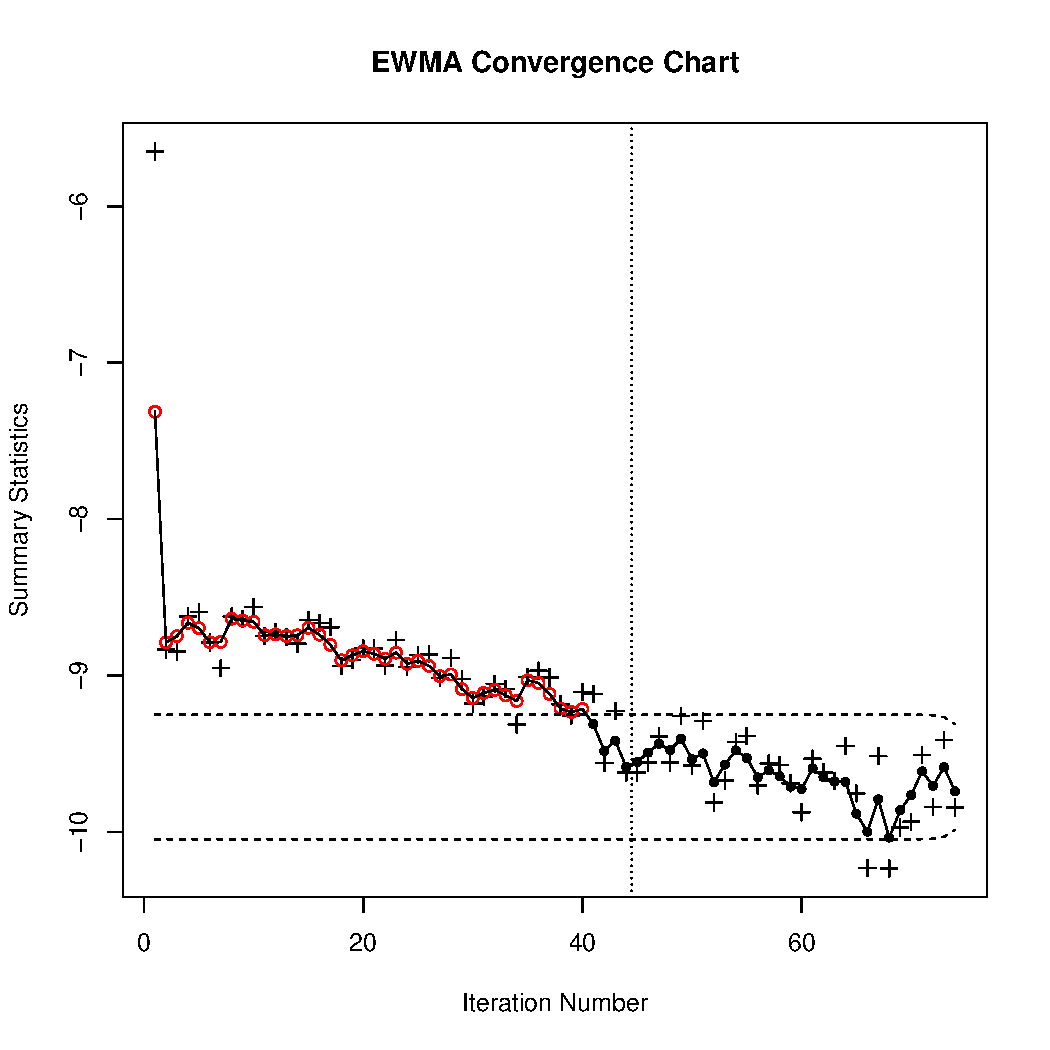
\includegraphics[width=0.32\textwidth]{./figures/ewmaConvChartRoseEasyEasyOpt.pdf}
%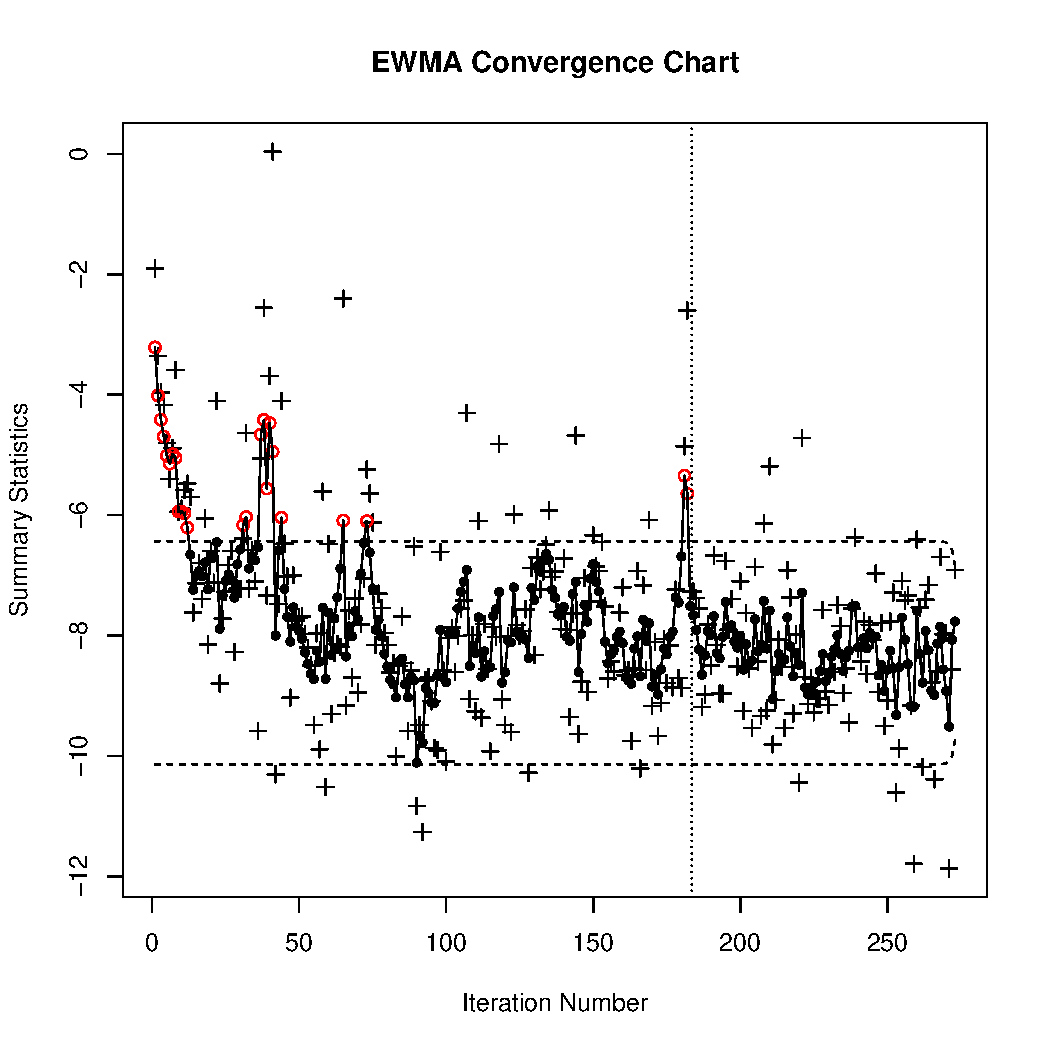
\includegraphics[width=0.32\textwidth]{./figures/ewmaConvChartLock6Three20000Opt.pdf}
%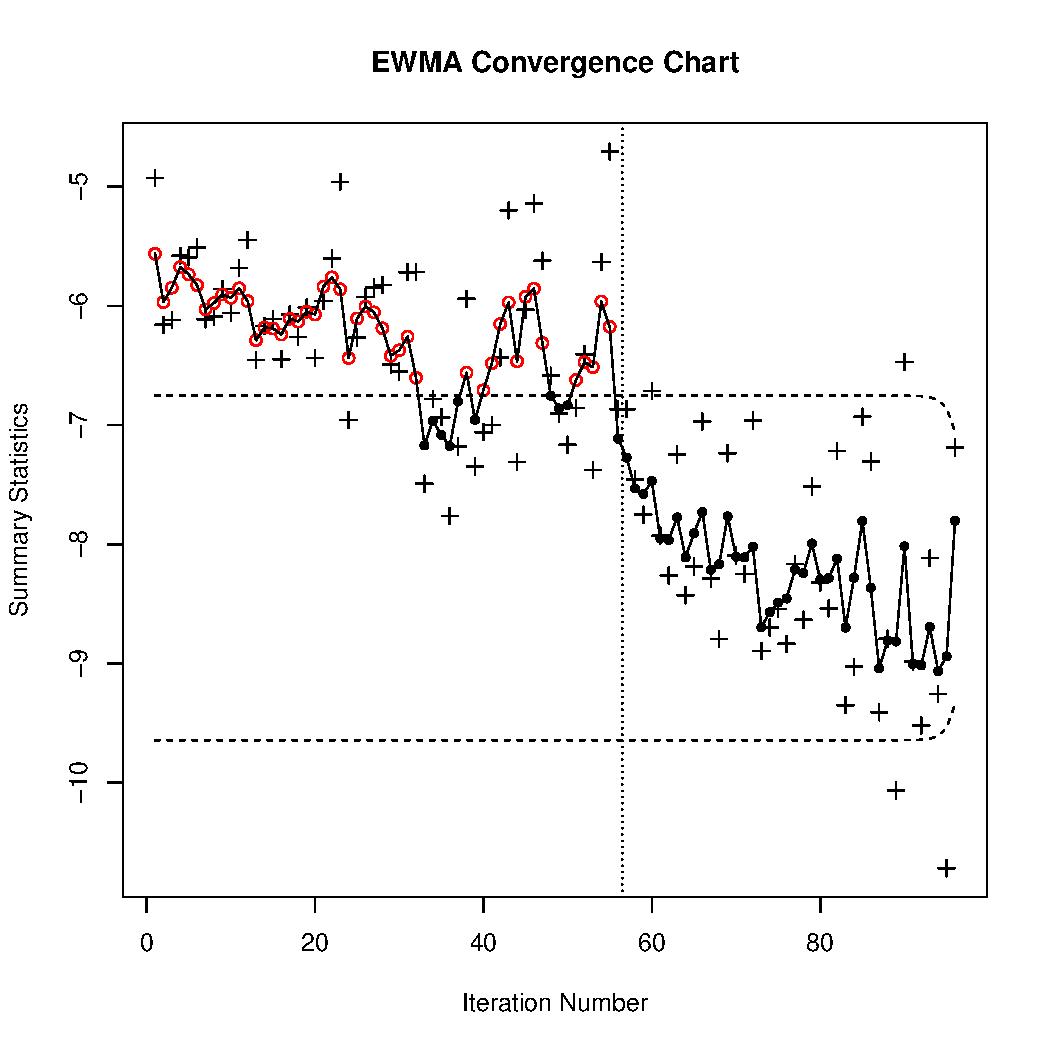
\includegraphics[width=0.32\textwidth]{./figures/ewmaConvChartRastHardOpt.pdf}
%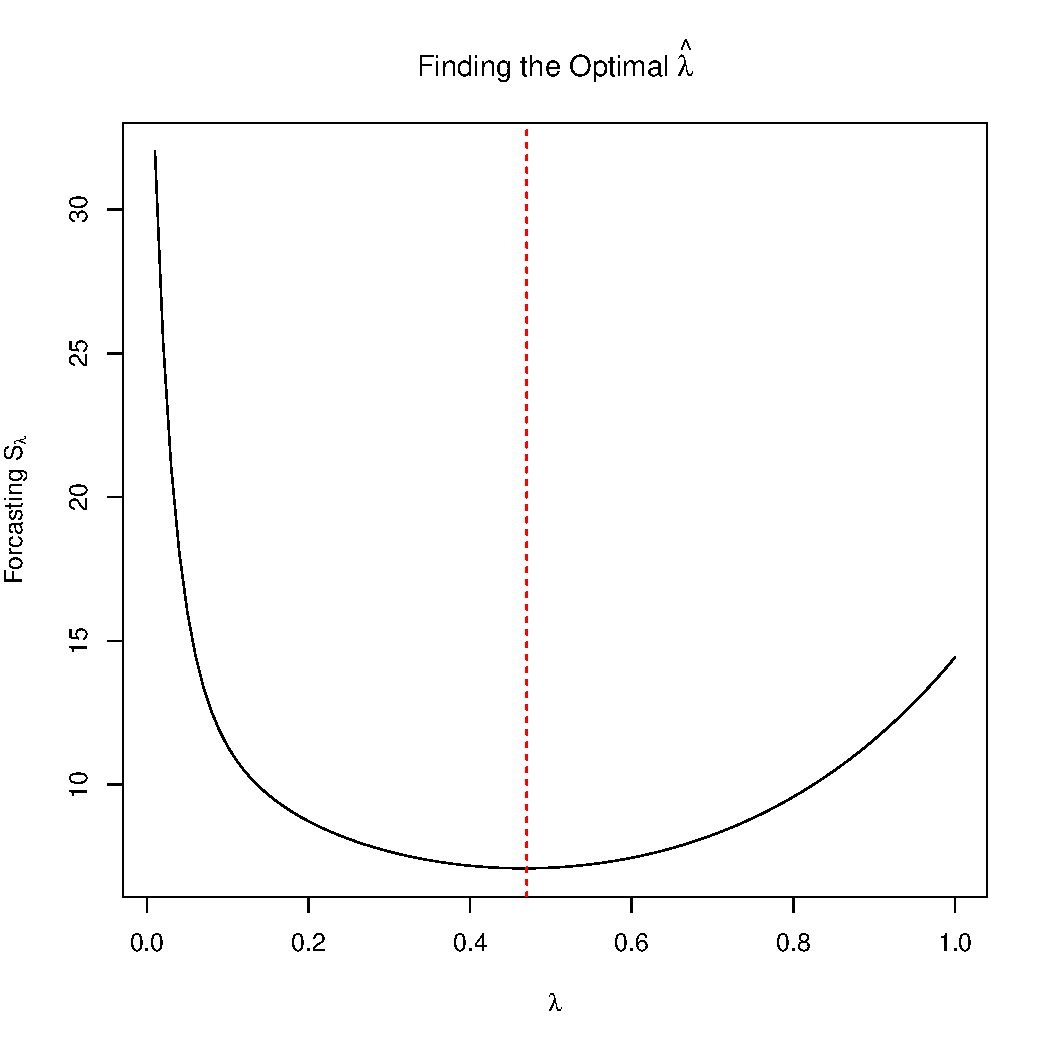
\includegraphics[width=0.33\textwidth]{./figures/ssRoseEasyEasyOpt.pdf}
%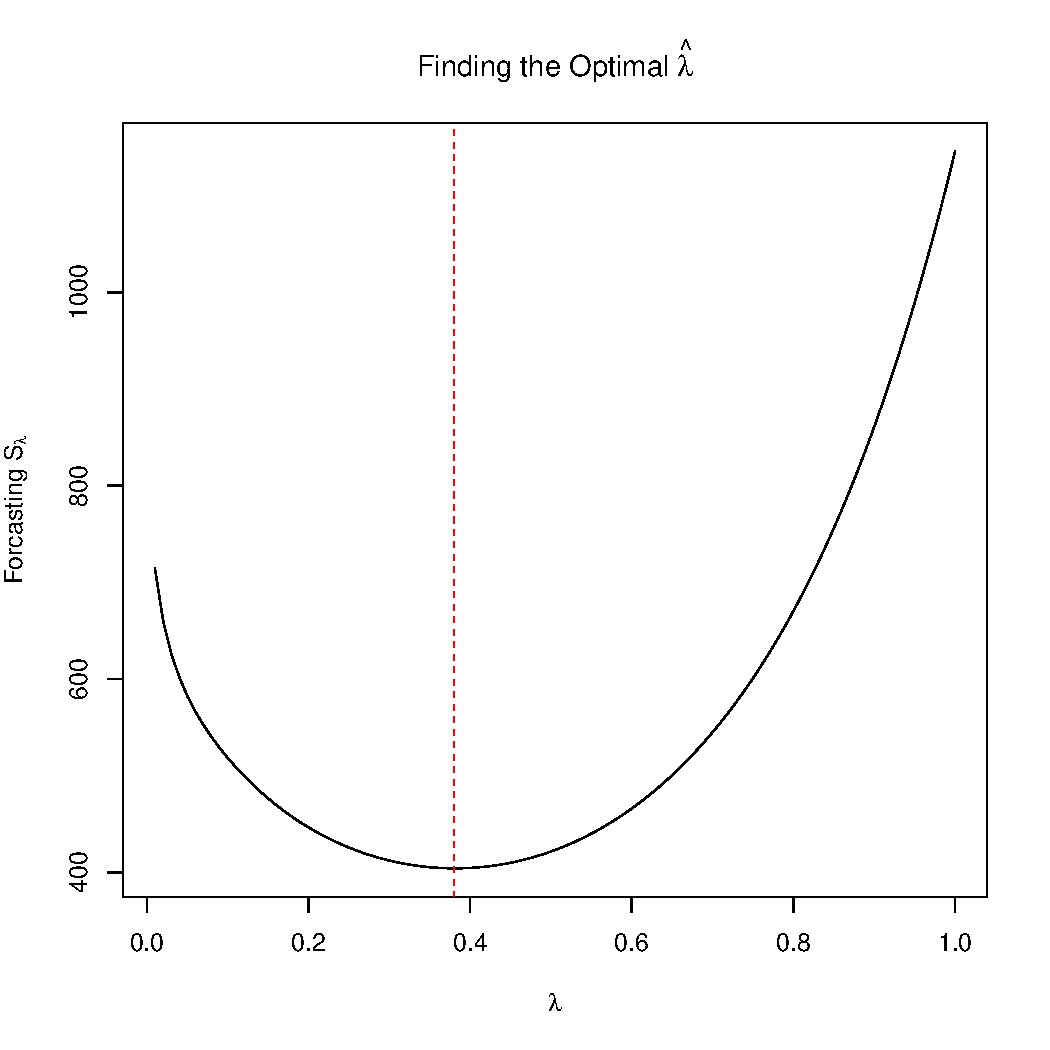
\includegraphics[width=0.33\textwidth]{./figures/ssLock6Three20000Opt.pdf}
%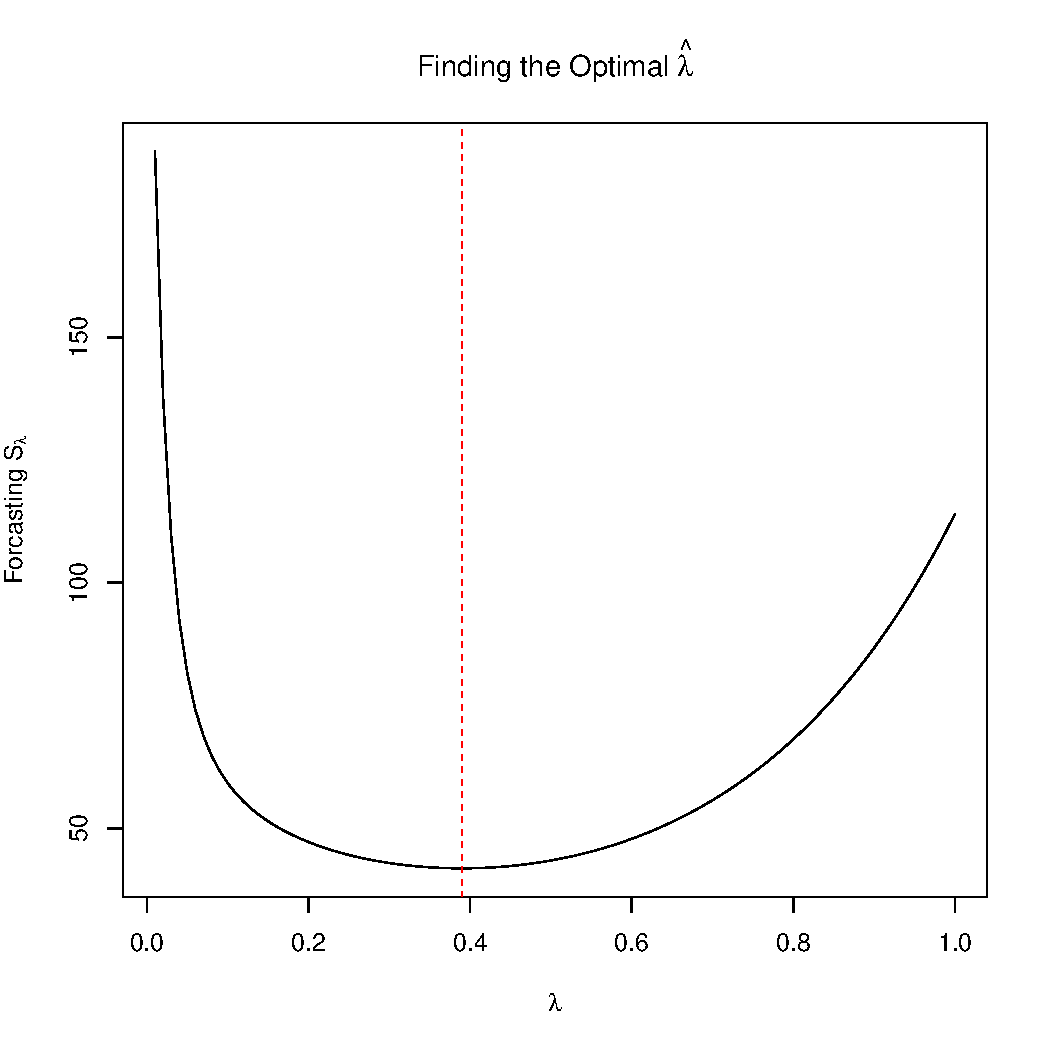
\includegraphics[width=0.33\textwidth]{./figures/ssRastHardOpt.pdf}
%\caption{$left:$ Rosenbrock | $center:$ Lockwood | $right:$ Rastrigin}
%\label{ewmaFig}
%\end{figure}
%%
%%

%
%\clearpage
%
%
\section{Examples}
\label{sec:examples}
%
We first look at two synthetic examples from the optimization literature, where the true optimum is known, so we can be sure we have converged to the true global minimum.  
%
We then provide a real world example from hydrology.

%
%
\subsection{Rosenbrock}
%
%

%
The Rosenbrock function \cite{rosePaper} was an early test problem in the optimization literature. 
%
It combines a narrow, flat parabolic valley with steep walls, and thus it can be difficult for gradient-based methods. It is generalizable to higher dimensions, but we use the two-dimensional version here.
%
\begin{center}
	%\label{roseFig}
	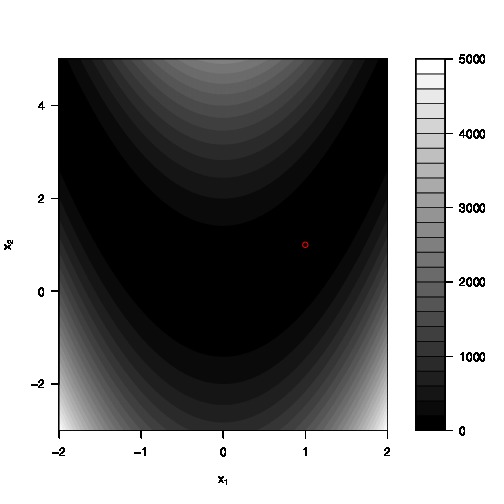
\includegraphics[width=0.5\textwidth]{./figures/roseContourBW.jpg}
	\begin{eqnarray}
	f(x_1, x_2) &=& 100\left(x_2-x_1^2\right)^2 + (1-x_1)^2 \\
	\text{Minimum}&:& f(1, 1)=0\nonumber
	\label{roseEq}
	\end{eqnarray}	
\end{center}
%
Convergence is non-trivial to assess, because optimization routines can take a while to explore the relatively flat, but non-convex, valley floor for the global minimum.  
%
Here we focus on the region $-2\le x_1\le2$, $-3\le x_2\le5$.  
%
While the region around the mode presents some minor challenges, this problem is unimodal, and thus represents a relatively easier optimization problem.  
%
This example illustrates a well-behaved convergence process.

\begin{figure}[htb]
  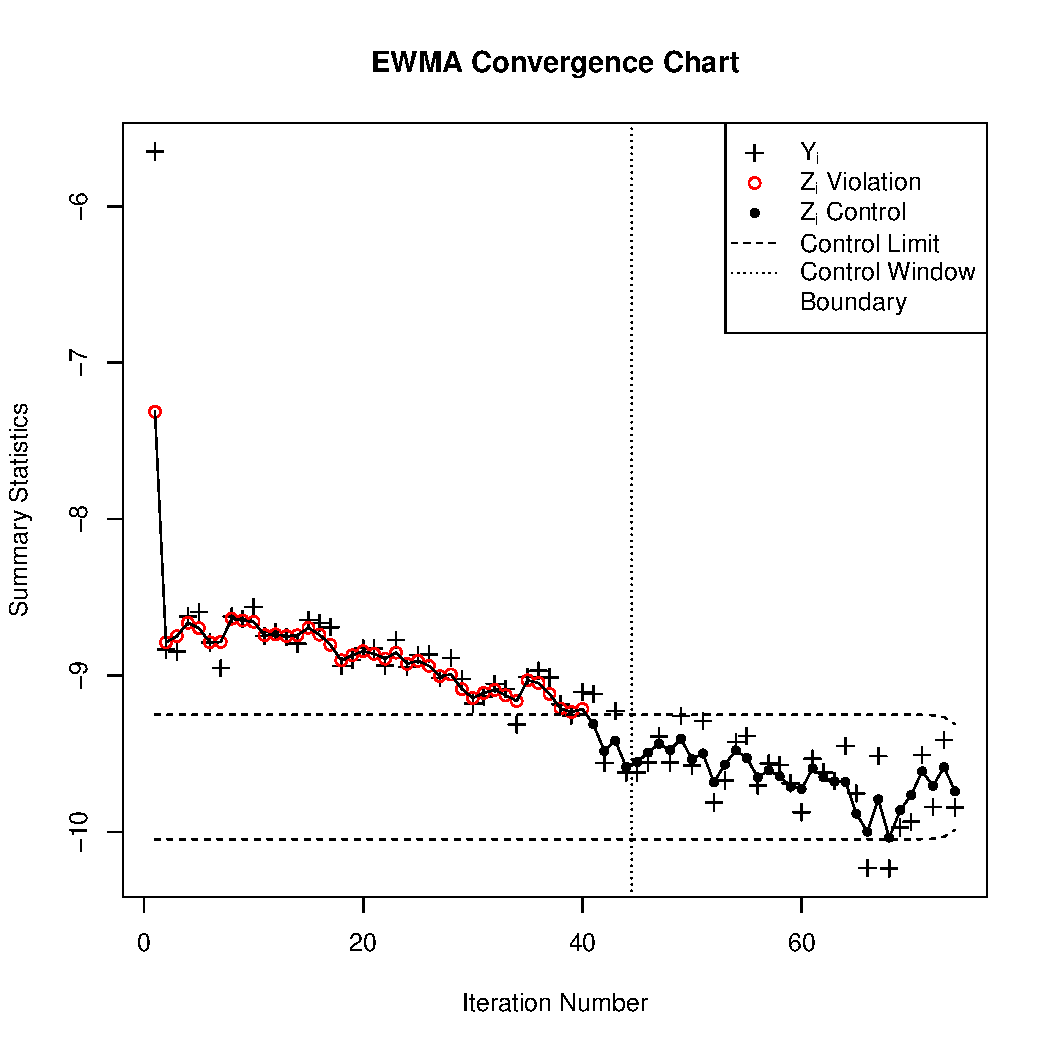
\includegraphics[width=0.45\textwidth]{./figures/ewmaConvChartRoseEasyEasyBW.pdf}
  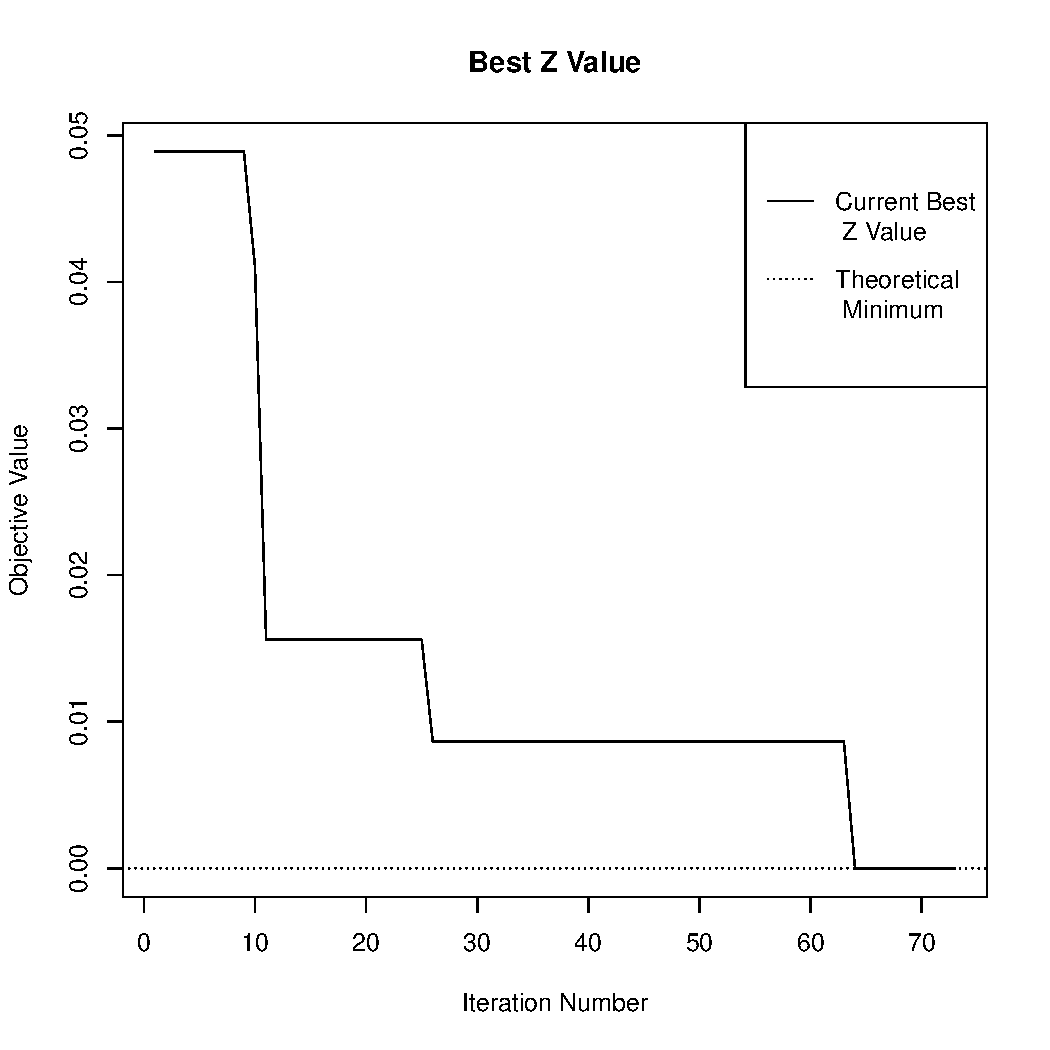
\includegraphics[width=0.45\textwidth]{./figures/bestZRoseEasyEasyEnd.pdf}
  \caption{Rosenbrock function: Convergence chart on the left, optimization progress on the right.}
\label{fig:rosenbrock}
\end{figure}
%use default values for our convergence parameters, $\lambda=0.2$ and $w=30$.
We estimate $\lambda$ via the minimum $S_\lambda$ estimator, $\hat\lambda\approx\roseLamb$, and use the minimum default value $w=30$.
%
Figure~\ref{fig:rosenbrock} shows the result of surrogate model optimization at convergence, as assessed by our method.  
%
The right panel shows the best function value ($y$-axis) found so far at each iteration ($x$-axis), and verifies that we have found the global minimum. 
%
The left panel shows our convergence chart, with the window indicated by the vertical line.  
%
The dashed horizontal lines show the control limits. 
%
At iteration 74 is the first time that all EWMA points in the control window are within the control limits, and thus we declare convergence.  
%
Note that the EWMA points generally trend downward until the global minimum has been found.  

%
%
\subsection{Rastrigin}
%
%

%
The Rastrigin function is a commonly used test function for evaluating the performance of global optimization schemes such as gentetic algorithms \cite{rastCite}.
%
The global behavior of Rastrigin is dominated by the spherical function, $\sum_i x_i^2$, however Rastrigin has been oscillated by the cos(.) function, and shifted, so that it achieves a global minimum value of 0 at the lowest point, of its lowest trough at (0, 0).

%
%
\begin{center}
        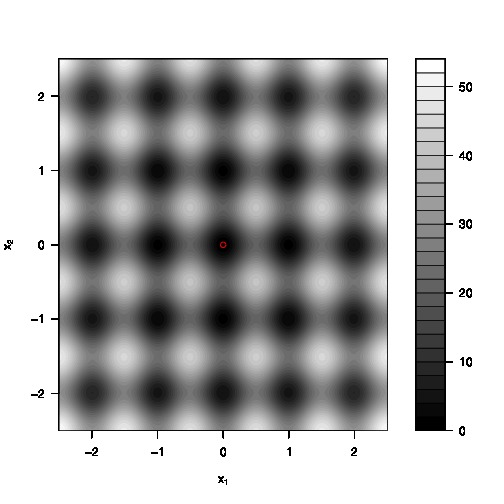
\includegraphics[width=0.5\textwidth]{./figures/rastContourBW.jpg}
	\begin{eqnarray}
	f(x_1, x_2) &=& \sum_{i=1}^2\left[x_i^2-10\cos(2\pi x_i)\right] + 2(10)\\
	\label{rastEq}
	\text{Minimum}&:& f(0, 0)=0\nonumber
	\end{eqnarray}
\end{center}
%
%

%
Rastrigin is generalizable to an arbitrarly many dimensions, but to develop intution, this example considers Rastrigin over the 2 dimensional square $-2.5\le x_i\le 2.5$.
%
Rastrigin is a highly multimodal function, and as such, the many similar modes present a challenge for identifying convergence.
%
The multimodality of this problem increases the variablility of the EI criterion, and thus represents a moderately difficult optimization problem in this context. 
%
It should be noted that by increasing the size of the search domain, either by increasing the bounds of the search square and/or increasing the dimension of the domain would make this example considerably more difficult and a less intuitive example for developing the choice of $w$. %tuning parameters.

%
%
\begin{figure}[!htb]
	\centering
	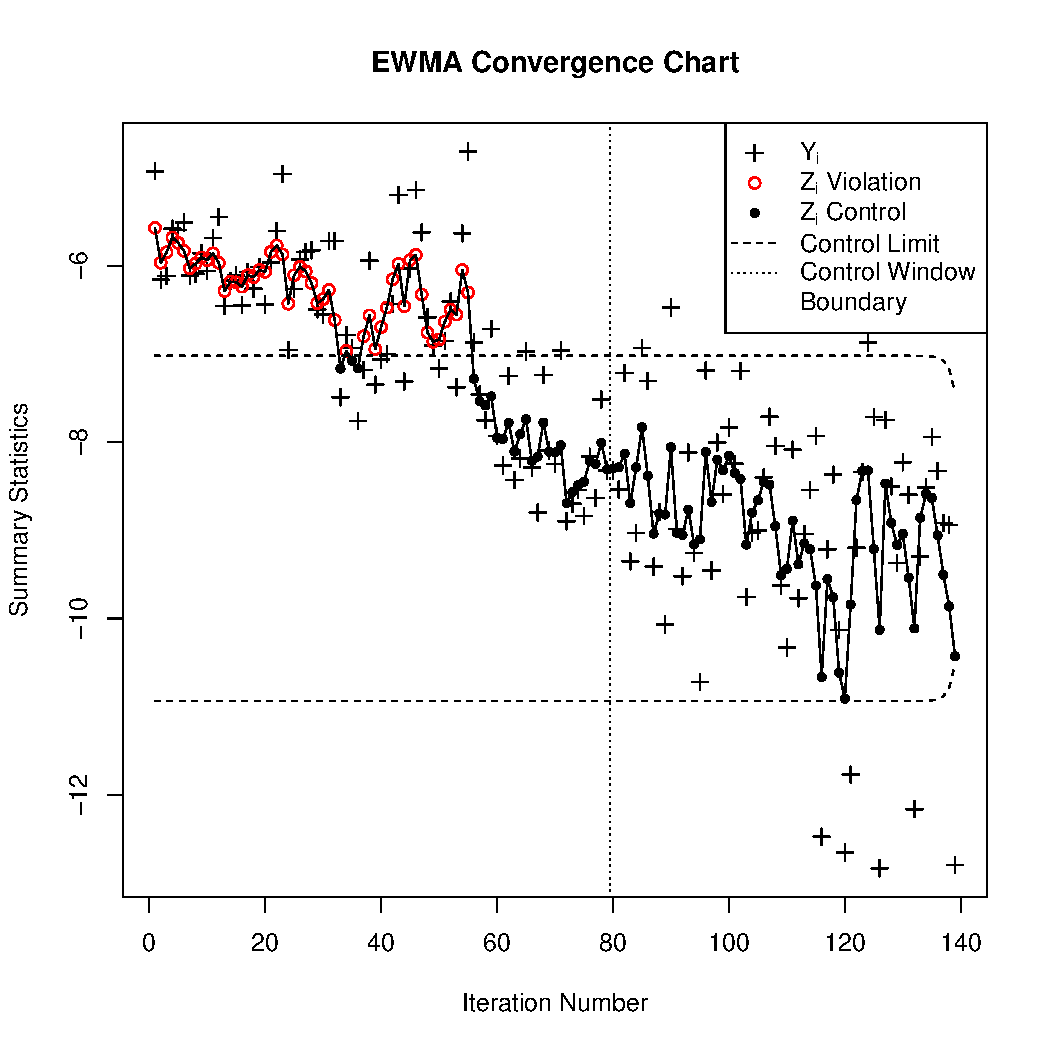
\includegraphics[width=0.45\textwidth]{./figures/ewmaConvChartRastHardBW.pdf}
	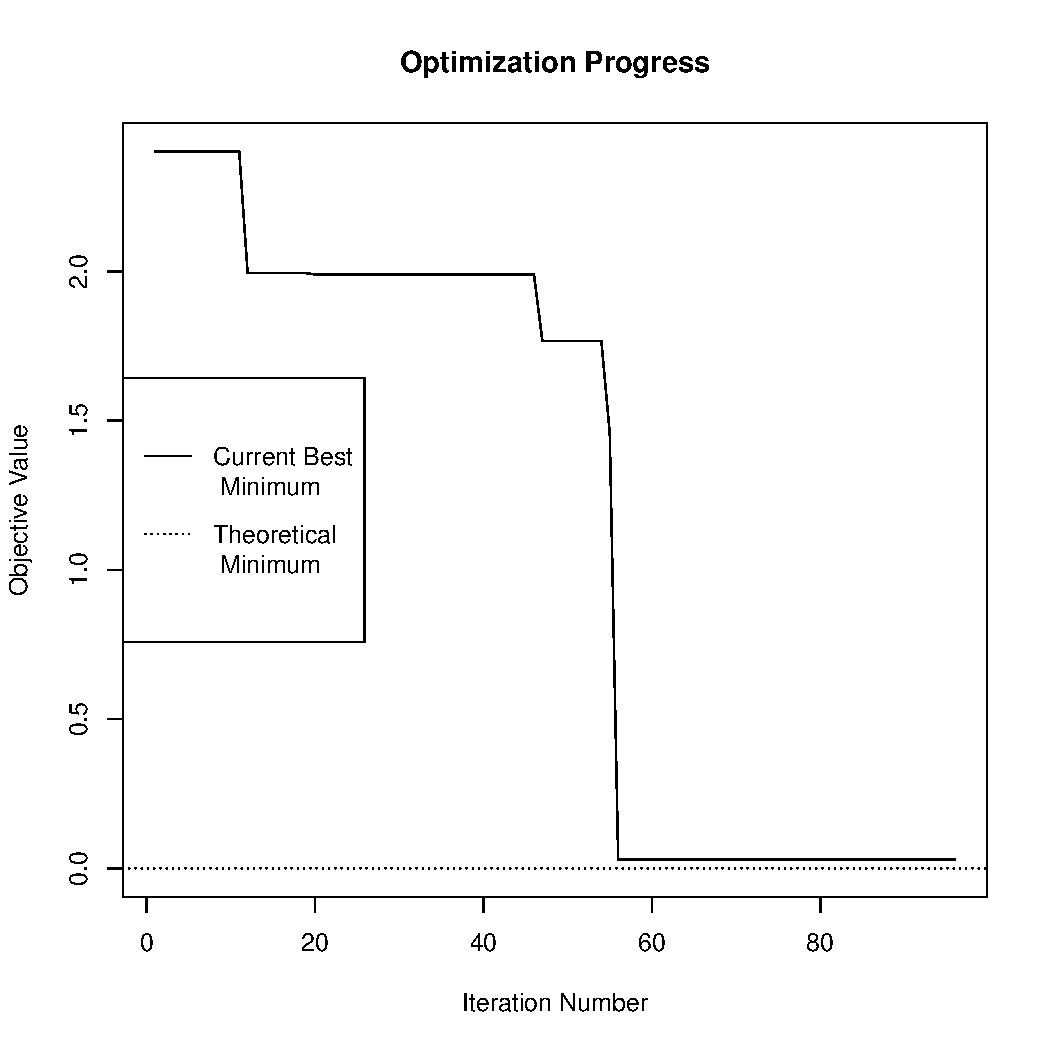
\includegraphics[width=0.45\textwidth]{./figures/bestZRastHardEnd.pdf}
	\caption{Rastrigin function: Convergence chart on the left, optimization progress on the right.}
	\label{fig:rastrigin}
\end{figure}
%
%

%
$\hat\lambda$ in this example is calculated to be about \rastLamb.
%
The decreased value of $\hat\lambda$, relative to Rosebrock, increases the smoothing capabilities of EWMA proceedure, as a response to the increased noise in th ELAI series.%so as to separate out the increase noise in the ELAI series from  signal.% the increased noise in the ELAI series to a greater degree, as values more by reflectes the increased use of $\lambda$ as a smoothing parameter, relative to rosebrock.
%
The added noise of the ELAI criterion, in this case, comes from the regular discovery of dramatic new modes as optimization proceeds.
%
Due to the increased complexity of Rastrigin relative to Rosenbrock, a larger $w$ is needed to recognize convergence in the presence of increased noise in the ELAI criterion. 
%
In this application $w=40$, was chosen by experimentation.
%
Although larger choices of $w$ produce equally consistent identification of convergence, they do so with more function evaluations.

%
%

%
Figure~(\ref{fig:rastrigin}) shows the convergence chart (left) and the optimization progress of the algorithm (right) after 95 iterations of optimization.
%
Although the variablity of the ELAI crterion increases as optimization proceeds, large ELAI values stop arriving after iteration 55, coincidently with the surrogate model's discovery of the Rastrigin's main mode, as see in the right panel of Figure~(\ref{fig:rastrigin}).
%
Furthermore notice that optimization progress in Figure~(\ref{fig:rastrigin}, right) demonstrates that convergence in this case does indeed represent approximate identification of the theoretical minimum of the the function, as indicated by the dashed horizontal line at the theoretical minimum. 

% has shown to be effective and smaller choices ofwas chosen here 
%as the  as the increased $\lambda$ attempts to forcast the large fluctuations of the ELAI criterion produced by the regular discovery of dramatic new modes.
%%
%Due to the increased complexity of the rastrigin function a larger $w$ is needed to recognize convergence in the presence of increased noise in the ELAI criterion do to

%
%Figure~(\ref{fig:rastrigin}) 
%
%
%Notice that the  
%Due to the increased complexity of the rastrigin function a larger $w$ is needed to recognize convergence in the presence of increased noise in the ELAI criterion do to 

%%
%\begin{itemize}
%%\item lambda choice
%%\item w choice
%\item results (when,where,bestZ fig)
%\item interesting tid-bits
%\end{itemize}

%
%
\subsection{Lockwood Case Study}
\label{sec:lockwood}
%
%

%closed form
The previous examples have focused on analytical functions with known minima.
%
This is done for the sake of developing an intuition for tuning the EWMA convergence chart parameters and to ensure that our methods correspond to the identification of real optima.
%However, in most practical optimization problems it is not possible to visualize to objective function so straight forwardly, or derive theoretical minima in this way.
%REVISE!!!!
%To demonstrate the use of the EWMA convergence chart in a practical optimization problem, 
Here we apply the EWMA convergence chart in the practical optimization setting of pump and treat optimization problems as formulated by Mayer et al. (2002) \cite{mayer2002optimal}.
%
Specifically we consider the Lockwood pump and treat problem, originally presented by Matott et al. \cite{lockCite}. %, and additionally presented \cite{gramacy2014}.

%
%

%%of contaiminted groundwater tha pumping site for chlorinated solvents located north-east of Billings, Montana, along the Yellowstone River.

The Lockwood pump and treat case study considers an industrial site, along the Yellowstone River, in Montana, with groundwater contaminated by chorinated solvents. %cothat has contaminated the surrounding groundwater with chlorinated solvents.%
%
If left untreated, this contaminated groundwater may contaminate the Yellowstone river, as dictated by the hydrology of the system. %ical models.
%Yellowstone riverthe site is close enough to the contaminate the Yellowstone river with  Clorinated solvents contaiminating the ground water in this region  , two plumes for pumping
Inorder to control this contaminated groundwater, a total of six pumps situated over two plumes, of the contaminated groundwater, are used to redirect groundwater away from the river to a treament facility.
%
Due to the cost of running these pumps, over a long period of time, it is desirable to determine how to best allocate the pumping effort amoung these pumps so as to determine the lowest cost pumping strategy to protect the river.
%
Pumping each of these six wells at different rates can drastically change the groundwater behavior, and  thus a numerical simulation of the system is required to predict the behavior of the system at a given set of pumping rates. %behavior of the of the ground%results in changes the complicated groundwater behahviors, that require the evaluation of a numerical simulation of the system to predict.
%
% from the groundwater does not reach the Yellowstone River.
%Plumes A and B contain two and four wells respectively.
%seen in Figure (\ref{lockSite}), contains two plumes for pumping, Plume A and Plume B, containing two and four wells respectively.
%
%The objective is to determine the lowest cost pumping rates for each of these six wells such that contamination from the plumes does not reach the Yellowstone River.

%
%

%
The objective function, $f(\bm{x})$, to be minimized in this case, can be expressed as the sum of the pumping rates for each pump (a quanity proportional to the expense of running the pumps in USD), with additional large penalties associated with any contamination of the river. % by each plume, $c_A(\bm{x})$, $c_B(\bm{x})$. %$c_A(\bm{x})$ and $c_B(\bm{x})$ indicating that the  
        %, is the cost of operating the pumps, in USD; additionally, $f$ heavily penalizes solutions that contaminate the river.
\begin{equation}
f(\bm{x}) = \sum_{i=1}^6 x_i +  2\big[ c_a(\bm{x}) + c_b(\bm{x}) \big] + 20000 \big[ \oner_{c_a(\bm{x})>0} + \oner_{c_b(\bm{x})>0} \big] 
\label{lockLoss}
\end{equation}
%with simple search boundaries, \mbox{$0\le x_i\le20,000$} set for each pumping rate.
Here $c_a(\bm{x})$ and $c_b(\bm{x})$ are outputs of a simulation, indicating the amount of contamination, if any, of the river as a function of the pumping rates, $\bm{x}$, for each of the six wells.
%
Any amount of contamination of the river results in a large stepwise penalty which introduces a discontinuity into the objective function, at the contaimination boundary.
%Penalties associated with any contamination of the river are chosen to be large, so as to never gi enough to 
%
%, \mbox{$\left[x_1, ..., ~x_6\right] = \left[Q_{A1}, ~Q_{A2}, ~Q_{B1}, ~Q_{B2}, ~Q_{B3}, ~Q_{B4}\right]$}.
Each $x_i$ is bounded on the large interval, \mbox{$0\le x_i\le20,000$}, representing a large range of possible management schemes.
%
The full problem defines a six-dimensional optimization problem, to determine the optimal rate at which to pump each well, so as to minimize the loss function defined in Eq~(\ref{lockLoss}).
%
Since the loss function is defined over a large and continuous domain, and running the numerical simulation of the system is computationally expensive, this example presents an ideal situation for use with surrogate model based optimization. 
%to understand the behavior of the EI criterion I first consider simplified into%with respect to $f$;
%The two-dimensional problem provides a nice setting for understanding the a simplified version of EI behavior, and furthermore the simplified setting develops an expectation for the EI behavior in the full \mbox{six-dimensional problem.}



% \begin{itemize}
% \item Describe case study
% \item general shape characteristcs os loss function
% \end{itemize}
% 
% %
% {\color{red} insert loss function, and some visualization}
% \begin{equation}
% f(\bm{x}) = \sum_{i=1}^6 x_i +  2\big[ c_A(\bm{x}) + c_B(\bm{x}) \big] + 20000 \big[ \oner_{c_A(\bm{x})>0} + \oner_{c_B(\bm{x})>0} \big] 
% \end{equation}
%

%\begin{itemize}
%%\item describe search domain
%\item ~~~ describe challenges ~~~
%\end{itemize}

%
%%ewmaConvChartLock6Three20000.pdf
\begin{figure}
	\centering
	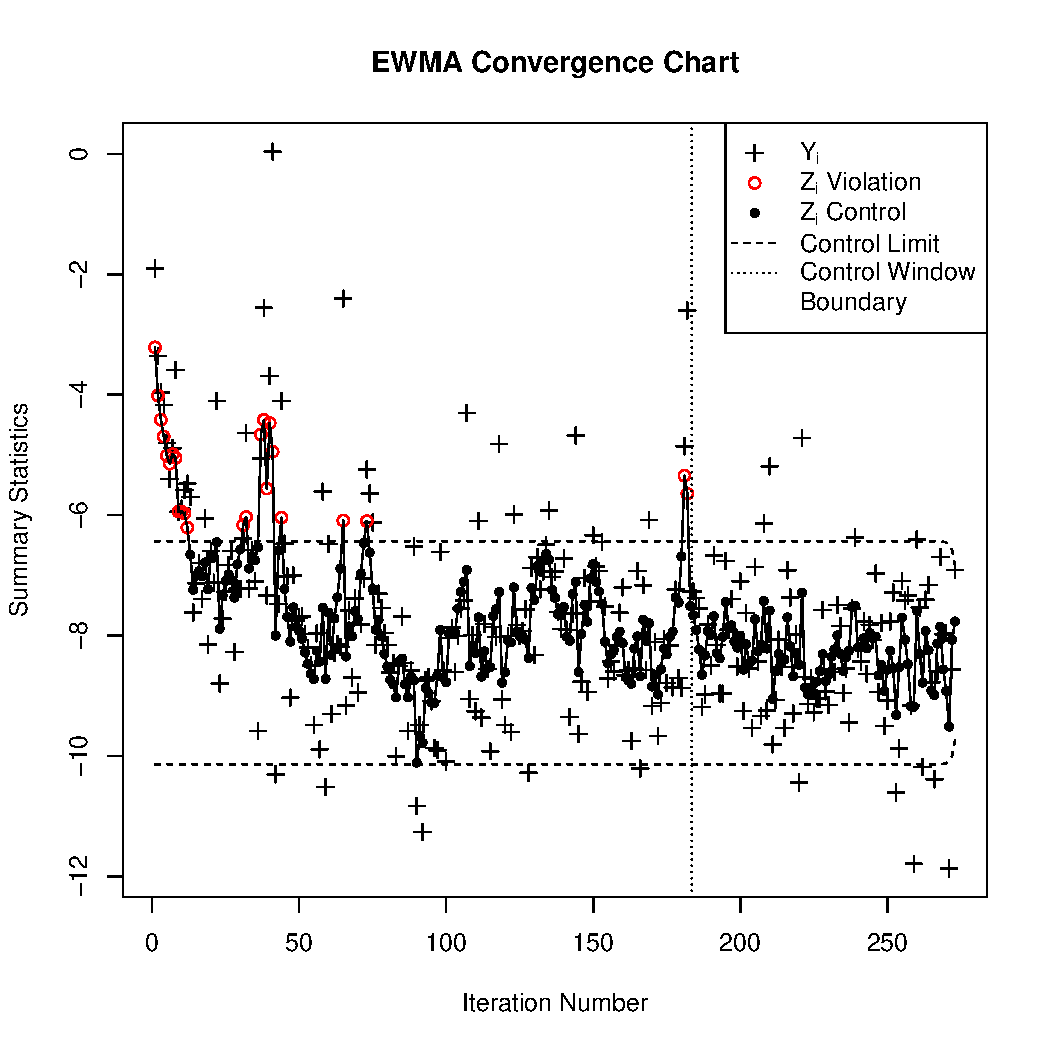
\includegraphics[width=0.45\textwidth]{./figures/ewmaConvChartLock6Three20000End.pdf}
	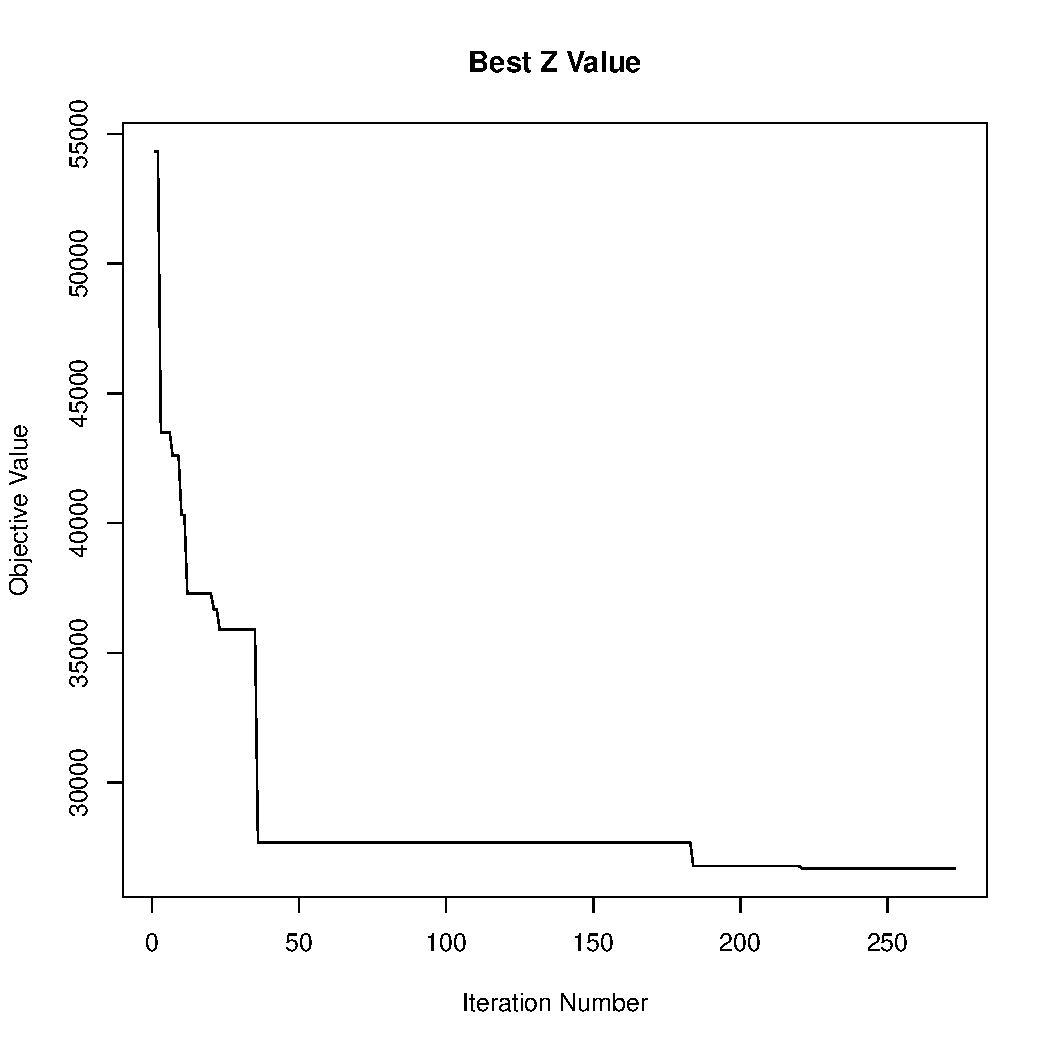
\includegraphics[width=0.45\textwidth]{./figures/bestZLock6Three20000End.pdf}
	\caption{Lockwood Case-study: Convergence chart on the left, optimization progress on the right.}
	\label{lock6EWMAEnd}
\end{figure}
%
%

%
Again $\lambda$ was chosen via the minimum $S_\lambda$ estimator to be $\hat\lambda\approx\lockLamb$ in this case.%, cooroborating  
%
This level of smoothing is required here to reduce the noise in ELAI criteion due to the large search domain, as well as the complicated contamination boundary amoung the six wells.
%
Furthermore these featres of the objective function complicate fit of the surrogate model and thus more function evaluations are required to produce an accurate model of $f$. %  accurately  the of the  dificultie
% to get a enough information to provide  to gather enough information to  was chosen to be 90 iterations of the algorithm to provide the 
%to produce, to yeild
As a result, the control window size, $w$, must increase to provide the initial surrogate model enough information to yeild reasonable accuracy. 
%determined, demonstrated, established, indicated, validated, corrobotated
Here $w$ was chosen to be 90 iterations, as determined by the adequate initial surrogate model behaviour as well as consistent identification of convergence.

%
%

%
The convergence chart for monitoring the optimization of the lockwood case study, is shown in the left panel of Figure~(\ref{lock6EWMAEnd}), as computed with $\hat\lambda\approx\lockLamb$ and $w=90$.%  $ (left) and optimization progress
%
Convergence in this case does not occure with a dramatic shift in the mean level of the ELAI criterion, but rather convergence occures as optimization the series stabalizes after large ELAI value move beyonfd the control limit.%, and  
%
Interestingly the last major spike in the ELAI series is observed alongside the disovery of the final major jump in the current best minimum value as seen at about iteration $180$ in the right panel of Figure~(\ref{lock6EWMAEnd}).
%
The EWMA convergence chart identifies convergence as the EWMA statistic associated with this final ELAI spike eventally exits the control window at iteration $270$.
%
The solution shown here corresponds to $f(\bm{x})\approx26696$ at $\bm{x}\approx[0, 6195, 12988, 3160, 1190, 3163]$.
%
This solution is well corroborated as a point of dimishing returns for this problem, by the analysis of Gramacy et al. \cite{gramacy2014} on the same problem, as seen their average EI surrogate modeling behavior. %gorithms as guided by the EI criterion.

%In Figure (18, right), after about 210 iterations, the algorithm finds its lowest cost solution to be seen in 500 iterations, corresponding to f (x) ≈ 26696 at x ≈ [0, 6195, 12988, 3160, 1190, 3163]. 
%Considering Figure (18, left), the EWMA convergence chart identifies this convergence after only about 270 iterations.
%%
%%
%%
%Figure~(\ref{fig:rastrigin}) shows the convergence chart (left) and the optimization progress of the algorithm (right) after 95 iterations of optimization.
%%
%Although the variablity of the ELAI crterion increases as optimization proceeds, large ELAI values stop arriving after iteration 55, coincidently with the surrogate model's discovery of the Rastrigin's main mode, as see in the right panel of Figure~(\ref{fig:rastrigin}).
%%
%Furthermore notice that optimization progress in Figure~(\ref{fig:rastrigin}, right) demonstrates that convergence in this case does indeed represent approximate identification of the theoretical minimum of the the function, as indicated by the dashed horizontal line at the theoretical minimum. 

%
%\begin{itemize}
%%\item lambda choice
%%\item w choice
%\item results (when,where,bestZ fig)
%\item interesting tid-bits
%\end{itemize}
%

\clearpage
%
%
\section{Conclusion}
%
%

%
Adapting the notion of control from the SPC literature, the EWMA convergence chart outlined here aims to provide a objective standard for identifying convergence.%provides an objective definitionof convergence. 
%
The examples provided demonstrate how the EWMA convergence chart may accurately, and efficiently, identify convergence in the context of statistical surrogate model optimization.

%
%

%characterization
As for any optimization algorithm, a converged solution may only be considered as good as the algorithms consideration of $f$. 
%
Thus poorly tuned surrogate modeling strategies may never optimize $f$ to their fullest extent, but the EWMA convergence chart presented here may still claim convergence in these cases. % algorithms. 
%
The EWMA convergence chart may only consider convergence in the context of the algorithm in which it is imbeded, and thus should be interpreted as a means of identifying when an algorithm has converged rather than when the lowest minimum has been found. % only identify convergence relative to the quality
%
%In cases of poorly tuned algorithms, the EWMA convergence chart presented here may only identify convergence with respect to the quality of the particular surrogate modeling strategy used. 
%may often 
For poorly tuned surrogate modeling strategies the EWMA convergence chart may only identify that the algorithm has reached a point of diminishing returns; for correctly tuned surrogate modeling strategies this point should correspond with the realization of an optimal solution. 
%
In either poor or correct surrogate tuning, the EWMA convergence chart identifies the moment at which it is beneficial to stop iterating the routine and reflect upon the results.

%
%

%%
%Of course the methods shown here are not presented in the absence of their own parameters that require tuning, But I veiw these added parameters in Archemedies' spirt of replacing hard problems with a series of easier ones. 
%%

%
%

%
Admmitadly the use of the EWMA convergence chart comes with the addition of it's own parameters which themselves require estimation.
% 
The addition of these parameters can be easily justified under a divide and conquer mentality; thus replacing the original large subjective task of appropriatly identifying convergence with relatively simple parameter estimation problems. 
%
The choice of $\lambda$ has been shown to be relatively robust to suboptimal choices, and furthermore estimation of the minimum sum of the squared forcasting errors $\hat\lambda$ is a simple in practice.
%
The estimation of $w$ is more subtle, but follows from reasonable intuition of the problem.
%
The choice of $w$ would ideally consider an objective measure of the complexity of $f$ as well as the dimensionality of the domain, $p$.
%
%Fully characterizing the relationship between $w$ and the dimensionality and complexity of $f$ for choosing would require a large simulation experiment many possible objective function   
%
For simplicity the recommendation $w\ge15p$ has shown to work quite well, although it contains no explicate consideration of the observed complexity of $f$. 
%The rational being that the current methods for appropriate identification of convergene is a rather subjective task and 
%The choice of the EWMA convergence chart parameters, $w$ and $\lambda$,  
%Tuning the parameters 
%These methods are not presented in the absence of 

\begin{itemize}
\item tuning parameters added in the spirit of reducing hard problems into a series of esier ones
	\begin{itemize}
	\item convergence is hard and massively subjective
	\item interpreting convergence charts is easier
	\item tuning $\lambda$ is objective and robust
	\item tuning $w$ can be subjective (requires large simulation study to choose.)
	\end{itemize}  
\item choose $w$
	\begin{itemize}
	\item complexity of $f$ (??entropy??)
	\item Dimension of $f$
	\item Emplerical results here: $w\approx 15p$; $p$ is the dimension
	\end{itemize}
{\color{red}
\item 2-parameter box-cox EI transformation instead of ELAI}
\end{itemize}

%
%
%VVV --- Masters Project --- VVV
%
%

% 	%
% 	Convergence is a bit of a loaded word, that is used in many different quantitative contexts.
% 	%
% 	In many cases the notion of ``convergence'' can be a frustratingly soft idea, often with an oddly subjective definition and fuzzy interpretation.  
% 	%
% 	In each different context of the word, ``convergence'' may have a slightly different meaning, and with it, ``convergence'' may carry different implications about the problem at hand.
% 	%typical definition implications
% 	Within the setting of optimization, convergence usually just indicates that we can stop iterating our routines, but even within optimization, convergence can look drastically different from routine to routine.
% 	%
% 	In this paper I aim to give ``convergence'' a more concrete definition in the context of Gaussian process surrogate model optimization.
% 	
% 	%
% 	%
% 	
% 	% an equally stochastic nature. in this context is thus  stochastic in nature thus
% 	By the nature of the stochastic exploration procedures inherent to Gaussian process surrogate model optimization, convergence is also stochastic in nature. 
% 	%
% 	Unlike other methods, such as gradient descent or pattern search, convergence in Gaussian process surrogate model optimization is not as straightforward as monitoring a vanishing step-size.
% 	%
% 	In Gaussian process surrogate model optimization the step-size, between locations of function evaluations, is a largely varied random variable and thus it is not a particularly telling feature of the progress of the objective search.
% 	%
% 	Among many practical surrogate modeling applications the claim of convergence may simply depend on the available computation time and the adequacy of the current best solution.
% 	%Rather,
% 	However it is obviously preferred to have metrics which expressly indicate convergence.
% 	%have often been used in a case-by-case manner to ad hocly diagnose convergence .
% 	For this purpose, various secondary criteria \cite{gramacy2014}, derived from the surrogate model itself, have been monitored.
% 	%
% 	In particular it is common to monitor the maximum expected-improvement (EI) until it simply falls below a specified threshold \cite{windExample}.
% 	%
% 	This over simplifies the dynamics of convergence in this setting, as quite small EI values should be expected with some regularity based on the particular topology of the problem and the stochasticity of the criterion itself. 
% 	%
% 	For the purpose of formalizing a robust process for tracking this stochastic criterion, I turn to the charting methods of the statistical process control literature.
% 	%%an alize a concrete definition of convergence in this context.% give convergence a more objectively tangible definition.
% 	Here I borrow ideas from Shewhart's \cite{shewhartBook} classic notion of control, to chart the EI, and thus form a more accurate and objectively tangible definition of convergence.  
% 
% 	%
% 	%
% 	
% 	%the topics of optimization and Statistical Process Control (SPC),
% 	My argument is structured in the following way: Section 1.1 gives a brief overview of context for the optimization used here, Section 1.2 covers the basics of Gaussian process surrogate models, and Section 1.3 explains how these models have been used as efficient derivative-free optimization routines.
% 	%In Section 1.4 I introduce the use of $\EIx$ as a convergence criteria, and in Section 1.5 I provide a more in-depth discussion of the specific SPC charts needed to track this metric so as to consistently identify convergence.
% 	%$\EIx$$\EIx$ (EI)expected-improvement
% 	In Section 1.4 I introduce the use of EI as a convergence criterion, and in Section 1.5 I provide a more in-depth discussion of the statistical process control (SPC) logic I use to consistently identify convergence, via the EI criterion.
% 	%I use for
% 	In Section 2 I tie all of these topics together to outline a charting procedure to identify convergence in a robust way.
% 	% on several classic optimization test functions as well as {\color{red}on the Lockwood data}.
% 	Finally, in Section 3 I provide some examples of identifying convergence via the methods outlined in Section 2. 
% 	
% 	%
% 	%
% 	\subsection{Overview}
% 	%
% 	%
% 	
% 	%enormous best choice?{\color{red}enormously}
% 	Derivative-free optimization is an enormously practical and commensurately difficult task.
% 	%gradient descent is very eager, perhaps too eager to find optima
% 	Derivative information has the capacity to efficiently, and rather intuitively, lead the user to an optimal solution. %, as well as, the capability to signal that such an optimum has been found.
% 	%
% 	However, derivative information tends to be focused locally, around the starting location of the objective function search, and thus can easily get stuck at local optima.
% 	%
% 	Furthermore, derivative information is often not available in many practical problems.
% 	%
% 	%we are left quite literally no knowing which way is up :)
% 	When derivatives are not available we are left to find more creative ways of figuring out which way is up.
% 	%
% 	Examples of this creativity can be seen in the diversity of different techniques employed by some of the more popular methods for derivative-free optimization.
% 	
% 	%
% 	%
% 	
% 	%evolutionary/genetic; surrogate model
% 	Examples of effective, and greatly varying, derivative-free optimization strategies include: evolutionary algorithms (EA), simulated annealing (SA), pattern search (PS), trust region methods, as well as surrogate model approaches. 
% 	%
% 	Although widely varied, fundamentally these methods share three basic components \cite{noGradBook}.
% 	%new candidate points for evaluation of potentially optimal points.
% 	Firstly, there is some procedure for exploring the objective function space. 
% 	%
% 	Secondly, these methods use derivative-free information from exploratory function evaluations to update the exploratory procedure, and thus, explore more effectively.
% 	%
% 	Thirdly, a well rounded optimization routine is tasked with accurately identifying when it has found an optimal point.
% 	%
% 	By tweaking any one of these components, an optimization routine's behavior, with respect to scope, convergence, and accuracy, may differ dramatically.
% 	%
% 	Thus, an ideal optimization routine would explore a large space quickly, and it would tell you that it has converged to an accurate solution with minimal information required from the objective function.
% 	% optimization
% 	Of course, an optimization routine which embodies {\it all} of these characteristics does not exist, as of yet, but these are good characteristics to consider when choosing the best optimization routine for a particular problem.
% 
% 	%
% 	%
% 
% 	%of derivative-free optimization and identify convergence of
% 	In particular, I consider the convergence properties of Gaussian process surrogate model approaches.
% 	%
% 	The basic idea of surrogate model approaches is to create a statistical approximation (i.e. a model) of the objective function, and use this model to effectively search the objective landscape. 
% 	%
% 	Surrogate model-based approaches are primarily of interest due to their ability to deal with functions that are computationally expensive to evaluate because they take special care to minimize the number of objective function evaluations.
% 	%
% 	%The typical approach is to minimize the number of function evaluations needed, by using each function evaluation as data to construct a Gaussian process model of the objective function .
% 	The typical choice of model in the construction of a surrogate model-based optimization routine is a Gaussian process model \cite{gpSurrogate}.
% 	%
% 	%Gaussian 
% 	%The philosophy in the choosing a Gaussian process model comes from the parral spacial statistics 
% 	%
% 	The idea is to work out the next best point to explore by using the surrogate model instead of the objective function.
% 	%
% 	Working with the surrogate model saves objective function computation time, and further more, allows for a careful statistical search of the objective function. 
% 	%in Gaussian process surrogate model approaches; % surrogate model optimization schemes.
% 	I demonstrate how further analysis of Gaussian process surrogate models can be used to identify convergence in this setting.  
% 
% 	%
% 	%
% 	\subsection{Gaussian Process Models}
% 	%
% 	%
% 	
% 	%
% 	Gaussian Process (GP) models often arise naturally in the context of spatial statistics. 
% 	%their use b
% 	In fact, GP models often go by the name kriging due to Danie G. Krige who pioneered the use of GPs in the context of Geo-spatial data related to mining \cite{kriging}.
% 	%  subject of GP models (i.e. $f$)%it can often be instructive to visualize the process spatial
% 	Thus, it can often be instructive to think about the objective function, $f$, in the context of a spatial application rather than as an abstract mathematical function, since often times $f$ can resemble, or even actually represent, the classical spatial problems. 
% 	%and stationary% rethe mapping provided by $f$ is a reasonably smooth and stationary process for relating points in the domain, $\bm{x}$. %, by their relative distances from each other.
% 	The choice of a GP as a surrogate model for $f$ hinges on the fundamental idea that $f$ provides a reasonably smooth mapping for relating points in the domain, \textbf{x}, to response values, $z$(\textbf{x}). 
% 	%spatial reference?
% 	That is to say, if we have any hope of finding optima of $f$, we impose the idea that points close together in the domain should have values in the response that are predictably, and similarly, close.
% 	%might expect if $f$ represent  similarly based  characteristics $f$ were to represent a bringing these inferential biases into the model of
% 	Regardless of the true interpretation of $f$, by modeling $f$ in this way we may expect $f$ to behave, at least in part, as a spatial quantity; for instance $f$ may just as well represent the elevation of a mountain in space. 
% 	%
% 	
% 	%
% 	%
% 	
% 	% from a particular GP
% 	A formal statistical perspective expresses a GP as an infinitely dimensional generalization of the multivariate normal distribution, such that every realization of a GP is a normal random variable and jointly all such realizations form a multivariate normal distribution. 
% 	%
% 	Typically the mean response is modeled using a linear combination of simple basis functions, $\bm{\beta}^\intercal \text{\textbf{f(x)}}$, with a zero mean random process error term, $\epsilon$(\textbf{x}), such as,
% 	%
% 	\begin{equation}
% 	z(\bm{x}) = \bm{\beta}^\intercal \text{\textbf{f}}(\bm{x}) + \epsilon(\bm{x}) + \eta(\bm{x}).
% 	\label{baseEq}
% 	\end{equation} 
% 	%Here the $\bm{\beta}$ are trend parameters and  
% 	Here $\eta(\bm{x})$ is Gaussian noise, and $\epsilon(\bm{x})$ is fundamentally governed by a correlation function, $ K(\bm{x}, \bm{x}')$, such that the covariance is $C(\bm{x}, \bm{x}')=\sigma^2K(\bm{x}, \bm{x}')$. 
% 	%the distance between \textbf{x} and \textbf{x}$'$
% 	By specifying a homogeneous correlation function, we thus model the relationship of $||\bm{x}-\bm{x}'||$ with the correlation structure that we expect to see when jointly considering two such realizations of the GP.
% 	%For example, tone such 
% 	The following exponential power family provides a common example of such a choice of $K(\bm{x}, \bm{x}')$,
% 	%
% 	\begin{equation}
% 	K(\bm{x}, \bm{x}') = \exp\left\{ -\frac{||\bm{x}-\bm{x}'||^p}{d} \right\}.
% 	\label{corrFunc}
% 	\end{equation}
% 	%
% 	Considering Eq. (\ref{corrFunc}) for every combination of \textbf{x} and \textbf{x}$'$ among a particular data set provides a correlation matrix \textbf{K}; thus multiplying by $\sigma^2$ creates the likelihood covariance matrix \textbf{C}.
% 	%
% 	For further discussion of choices of $K(\bm{x}, \bm{x}')$ see \cite{steinBook}.
% 	%% Thus we can express this model in  equations (\ref{baseEq}) and (\ref{covFunc}) together as a proper Bayesian model we get,
% 	Equations (\ref{baseEq}) and (\ref{corrFunc}) imply the following simple Bayesian model, which forms the basis for many other complex GP models  
% 	%
% 	\begin{equation}
% 	\begin{aligned}
% 	\text{\textbf{Z}} ~|~ \bm{\beta}, \sigma^2, \text{\textbf{K}} &~\sim~ N_n\Big(\text{\textbf{F}}\bm{\beta},~ \sigma^2\text{\textbf{K}}\Big)
% 	&~ \sigma^2 ~|~ a, b &~\sim~ IG(a, ~b)
% 	\\
% 	\bm{\beta} ~|~ \bm{\beta}_0, \text{\textbf{V}} &~\sim~ N_m\big(\bm{\beta}_0,~ \text{\textbf{V}}\big) &~
% 	\text{\textbf{V}} ~|~ \bm{\Psi}, \nu &~\sim~ IW\big(\bm{\Psi}, ~\nu\big).
% 	\label{gpModel}
% 	\end{aligned}
% 	\end{equation}
% 	%
% 	Here $a$, $b$, $\bm{\beta}_0$, $\bm{\Psi}$, and $\nu$ are fixed hyper-parameters of the model, and $N$, $IG$, and $IW$ represent the Multivariate Normal, Inverse-Gamma, and Inverse-Wishart distributions respectively.
% 	%
% 	Model (\ref{gpModel}) specifies a mostly conjugate, Gibbs sampling, inference setting with the exception of the covariance structure parameters, which require Metropolis-Hastings sampling \cite{gpJasa}.
% 	
% 	%
% 	%
% 	
% 	%
% 	Bayesian models of this type, not only provide effective inference on $f$, but they provide a framework for prediction that allows for further efficient exploration of $f$.
% 	%
% 	In the Bayesian perspective, the parameters of Model (\ref{gpModel}) are random variables.
% 	% of these parameters over the parameters. allow a in the data
% 	Thus doing inference on these parameters, via MCMC, results not only in point estimates, but entire distributions that completely, and flexibly, describe the present uncertainty. 
% 	%
% 	%It is thus desirable to compute accurate empirical intervals based on these samples, rather than rely on the classical asymptotic theory.
% 	%
% 	%As to be discussed in section 2, the assumptions of the classical asymptotic theory may be hard to satisfy, and thus credible intervals are preferred here. 
% 	%sample based used to do inference on models like Model (\ref{gpModel})
% 	%that not only allows for
% 	Furthermore Bayesian methods, such as Model (\ref{gpModel}), provide a complete predictive framework for estimating function behavior in unobserved candidate locations, as well as full distributional uncertainty characterization of these unseen locations.
% 	%can be used to construct the posterior predictive distribution for new candidate locations of $f$.
% 	%several of which candidate locations may provide good potential of these 
% 	By considering the uncertainty and expected behavior of the posterior predictive GP surface across candidate locations, it is thus possible to make informed decisions about where to search for new optima \cite{taddyOpt}.
% 	
% 	%
% 	%
% 	
% 	%
% 	In many cases the assumption of a smooth $f$ with a homogeneous uncertainty structure can provide an effective and parsimonious model.
% 	%
% 	However for the sake of providing a flexible surrogate model, it is desirable to have the ability to loosen these restrictions in cases when $f$ looks more like the Grand Canyon, as opposed to the Great Plains.     
% 	%objective landscape
% 	Gramacy and Lee \cite{gpJasa} introduce the idea of allowing this flexibility via a treed partitioning of the domain.
% 	%
% 	This allows separately stationary GP surfaces to fit separately stationary portions of $f$.
% 	%
% 	For further explanation of partitioned Gaussian process models as well as notes on implementing such models in R, see the R package \verb tgp  \cite{tgp}.
% 	
% 	%\newgeometry{ margin=1in, footskip=0.4in }
% 	%\doublespacing
% 	%
% 	%
% 	\subsection{Optimization}
% 	%
% 	%
% 	
% 	%
% 	In explaining the construction of optimization routines based on statistical models like model (\ref{gpModel}) as described by \cite{taddyOpt}, I view the typical surrogate optimization procedure in terms of the three basic components of optimization that I outline in Section 1.1.1. 
% 	%
% 	Firstly, I identify the type of information that has been used in Gaussian process models to effectively explore $f$.
% 	%
% 	Secondly, I outline the exploration procedure, and how a Gaussian process updates its exploration of $f$ using this information.
% 	%\\\\
% 	For the sake of making a concrete argument, I focus
% 	on optimization in the context of minimization, but all of these ideas can easily be applied to finding maxima by simply minimizing $-f$.
% 
% 	%\restoregeometry
% 	%\doublespacing
% 	%
% 	%
% 	\subsubsection{Expected Improvement}
% 	%
% 	%
% 
% 	%$\Eix$ \cite{eiOpt},
% 	In finding minima via Gaussian process models, the expected-improvement (EI) criterion has been used \cite{tgp2}, \cite{taddyOpt} to identify candidate points that have the strongest {\it possibility of encountering new minima}.
% 	%when applied to a single candidate point has
% 	The EI criterion is fundamentally based on the improvement criterion for each candidate location of the following form,
% 	\begin{equation}
% 	\ix~=~ \max \Big\{ \big(f_{min} - f(\bm{x})\big), ~0 \Big\}
% 	\label{ix}
% 	\end{equation}
% 	%
% 	In expectation, the $\Eix$ criterion rewards candidate points not only for a low predictive mean, but also rewards the high uncertainty associated with poorly explored regions.
% 	%
% 	Considering Bayesian models like Model (\ref{gpModel}), we can most efficiently use information in our model by considering $\Eix$ with respect to the posterior predictive distribution.
% 	
% 	%
% 	%
% 	
% 	%
% 	%{\color{red}
% 	By the nature of the Bayesian construction of models like Model (\ref{gpModel}), criteria such as the improvement criterion, $\ix$, are random variables, and as such, we can learn their distributions via Markov Chain Monte Carlo (MCMC) methods.
% 	% each candidate location has a $\ix$ is a random variable, at each candidate location, who's distribution is easily accessible via the MCMC sample-based implementation of the model, as described in \cite{tgp}.
% 	%}Thus f; predictive For each candidate location t%, and using these samples to derive the .
% 	The distribution of $\ix$, a posteriori, can be obtained by considering samples from the posterior predictive distribution at each candidate location and computing the necessary statistics to form $\max \Big\{ \big(f_{min} - z(\tilde{\bm{x}})\big), ~0 \Big\}$ as an approximation of Eq. (\ref{ix}).  
% 	%\EIX is not quite right it should just be the single location formula
% 	Furthermore, the mean of these posterior predictive $\ix$ samples provide an empirical solution for finding an EI for each candidate location \cite{tgp2}.
% 	%same issue here EI criteria described in Eq. (\ref{EIx}), with $g=1$.
% 	Thus, truncating these $\ix$ samples at 0 and finding the candidate location with the maximum $\Eix$, identifies the EI criterion described.
% 
% 	%\clearpage
%         %
%         %
%         \subsubsection{Exploration Procedure}
%         %
%         %
%         
% 	%
% 	%
% 	\begin{wrapfigure}{r}{0.5\textwidth}
% 	\vspace{-1.6cm}
% 	%\vspace{-2.5cm}
% 	\singlespacing
% 	\caption{Optimization Procedure}
% 	\begin{itemize}
% 	\item[1)] Collect an initial set, $\bm{X}$.
% 	\item[2)] Compute $f(\bm{X})$.
% 	\item[3)] Fit GP model based on evaluations of $f$.
% 	\item[4)] Collect a candidate set, $\tilde{\bm{X}}$.
% 	%\item[5)] Compute $\Eix$ among $\tilde{\bm{X}}$.$\E{\text{I}(\tilde{\bm{x}_i}})$
% 	\item[5)] Compute EI among $\tilde{\bm{X}}$
% 	%\item[6)] Add $\tilde{\bm{x}_i}$ yielding largest $\Eix$ to $\bm{X}$.
% 	\item[6)] Add $\argmax_{\tilde{\bm{x}_i}} \E{\text{I}(\tilde{\bm{x}_i})}$ to $\bm{X}$.
% 	\item[7)] Check convergence.
% 	\item[8)] If converged exit. Otherwise go to 2).
% 	\end{itemize}
% 	\doublespacing
% 	%\vspace{-0.85cm}
% 	\label{procedure}
% 	\end{wrapfigure}
% 	%
% 	%
% 	
% 	% us with a
% 	The idea for optimization, in this context, is to only evaluate the objective function at locations that have a good chance of providing a new minimum. 
% 	%I need a handle
% 	An optimization scheme based on models like Model (\ref{gpModel}) starts by initially collecting a set, $\bm{X}$, of locations to evaluate the true function, $f$, to gather a basic impression of $f$.
% 	% (\ref{gpModel})
% 	A GP model is then fitted with $f(\bm{X})$ as observations of the true function.
% 	%EI
% 	Using this model, a set of candidate points, $\tilde{\bm{X}}$, are randomly selected from the domain and the EI criterion is calculated among these points.
% 	%
% 	The candidate point that has the highest EI is then chosen as the best candidate for a new minimum and thus, it is added to $\bm{X}$.
% 	% (\ref{gpModel})
% 	The objective function is evaluated at this new location and the GP model is refit based on the updated $f(\bm{X})$.
% 	%
% 	The optimization procedure carries on in this way until convergence.
% 
% 	
% 	%
% 	%
% 	\subsection{A Convergence Criterion}
% 	%
% 	%
% 	
% 	
% 	%
% 	Iterating the above mentioned optimization procedure and tracking the value of EI at each iteration gives the user a sense for what the algorithm thinks is left to learn about finding a minimum of $f$.
% 	%
% 	For instance, recall that EI is giving us information about the {\it possibility of encountering a new optimum}.
% 	%
% 	For determining convergence, you can imagine exploring $f$ with respect to EI, in the following way.
% 	%
% 	Initially, as we enter the objective landscape of $f$, we do not really know what to expect.
% 	%
% 	However we set-out to explore this space, and as we explore, we develop expectations about the topography of $f$.
% 	%
% 	Each exploratory sample of $f$ provides some potential for a new optimum, although as we learn more about this function, the expectation that we will see something new begins to diminish.
% 	%
% 	If we continue to explore\\ this landscape, we will come to understand the environment so well that we will virtually never expect to see something new.
% 	%
% 	In fact, continued exploration of the space may become boring.
% 	%that continued search of the objective function would be has become uninte
% 	Thus the key to efficiently identifying convergence is to quickly realize that the expectation of finding a new, and substantial, optimum is sufficiently low.
% 	%%would become uninteresting.
% 	That is to say, convergence occurs, in this context, when the expectation of finding new minima is low enough, so that continued search of the objective function is expected to be unproductive.
% 
% 	%\clearpage
% 	%
% 	%
% 	\begin{wrapfigure}{l}{0.5\textwidth}
% 	\vspace{-1.1cm}
% 	\begin{center}
% 	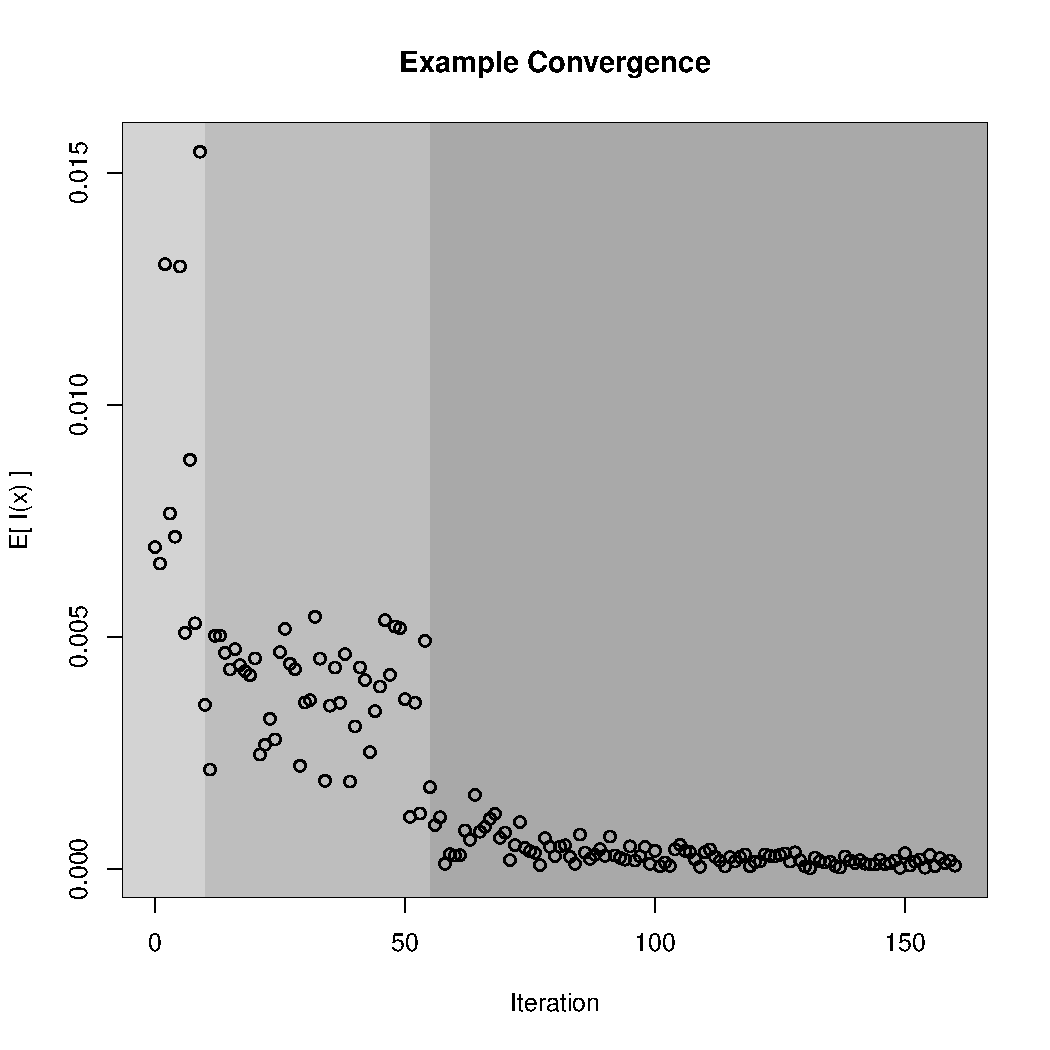
\includegraphics[width=0.5\textwidth]{./figures/exampleEI.pdf}
% 	\end{center}
% 	\vspace{-0.85cm}
% 	\caption{A fabricated EI progression, made to clearly demonstrate the typical three stage convergence pattern.}
% 	\label{EIxEX}
% 	\end{wrapfigure}
% 	%
% 	%
% 	
% 	%stochasticity
% 	Following from this intuitive story about the behavior of EI; quantitatively EI follows a stochastically non-stationary decreasing function as iterations of the optimization routine pass.
% 	%
% 	Initially EI tends to start in at an optimistically high value, depending on the initial size of $\bm{X}$.
% 	%
% 	As several iterations of the optimization procedure continue to sweep through, EI tends to enter a fairly stable region of intermediate values where the algorithm is figuring out the major features of $f$.
% 	%
% 	Eventually the value of EI will converge in probability to 0, but by construction it can not decrease below 0.
% 	
% 	%
% 	%
% 	\subsection{Statistical Process Control}
% 	%
% 	%
% 	
% 	%{\color{red}the elusively fuzzy concept of} %s sense of the word ``convergence''.
% 	In identifying convergence, I find the notion of ``control'', from the SPC literature, to be in the same spirit as the notion of ``convergence'' in optimization. 
% 	%
% 	In Shewhart's seminal 1931 book \cite{shewhartBook} on the topic of control in manufacturing, Shewhart explains that a phenomenon is said to be in control when, ``through the use of past experience, we can predict, at least within limits, how the phenomenon may be expected to vary in the future.''
% 	%
% 	This notion is not only an instructive framework for thinking about convergence, but it offers this framework with a comforting sense of finitude. 
% 	%
% 	The phrase ``within limits'' gives us a hope of drawing some line in the sand; turning the previously subjective burden of identifying convergence, into a simple objective task that even a computer can accomplish.
% 	
% 	%
% 	%
% 	
% 	%% of that statistic.
% 	In its most simplified form, SPC  considers an approximation of a statistic's sampling distribution as repeated sampling occurs in time.
% 	% from some data generating mechanism,
% 	For example, the $\bar x$-chart tracks the mean of, say $m$, repeated samples, of size $n$, so as to expect the arrival of each subsequent mean in accordance with the typical sampling distribution for the mean, $\bar{x}_j \sim N\left(\mu, \frac{\sigma^2}{n}\right)$.   
% 	%
% 	%Shewhart expresses his idea of control as the expected behavior of random observations from the sampling distribution of interest.
% 	Shewhart expresses his idea of control, in this case, as the expected behavior of random observations from this sampling distribution.
% 	%
% 	By considering confidence intervals on this sampling distribution we can easily draw explicit boundaries (i.e. control limits) to identify which samples are in control, and which are not.
% 	%
% 	Observations violating our expectations (i.e. observations that fall outside of our confidence interval/beyond the control limits) indicate an out-of-control state.
% 	%
% 	Since neither $\mu$ nor $\sigma^2$ are typically known, it is of primary importance to use the data carefully to form accurate approximations of these values, thus establishing a standard for control.
% 	%
% 	Furthermore, this logic relies upon the typical asymptotic results of the central limit theorem (CLT), and special care should always be taken to satisfy its requirements.
% 	
% %\clearpage
% %
% %
% \section{Identifying Convergence}
% %
% %
% 	
% 	%Considering Figure (\ref{EIxEX}) it is easy to see how tracking EI values could naturally fall into the framework of the SPC logic.
% 	Figure (\ref{EIxEX}) can bee seen to resemble an $\bar x$-chart, and with some modifications it is not hard see how tracking EI values could naturally fall into the framework of the SPC logic.
% 	%
% 	Recall that each point in this figure is the mean of $\ix$ MCMC samples at the most promising candidate location, in the current iteration.
% 	%as we look back through the previously observed EI values
% 	Thus as iterations of the optimization procedure pass, we form a repeated sampling situation for the EI values to consider via SPC.
% 	%presumably converged; new;  control for EI  state of control% is has presumably found convergence.
% 	The idea behind identifying convergence in this setting, is to establish a state of pre-convergence; we then claim that we have achieved convergence when we observe EI values that indicate a move from this pre-convergence state, into a state of control about some converged EI distribution. 
% 	
% 	%
% 	%
% 	
% 	%
% 	Considering the EI values in this way requires tactful consideration of how to evaluate the arrival of EI observations.
% 	%
% 	%Since it is not known when we may stumble across convergence we must be on the lookout for convergence in each iteration 
% 	%
% 	In order to achieve the above described perspective of convergence, the goal is to establish control among the most recently observed EI values as they move from the initial pre-convergence values into control.
% 	%look back through the EI values observed thus far in reverse order.
% 	Thus, it is necessary to consider the progression of EI values in the reverse order for the sake of SPC. %,  with the most recent observations 
% 	%
% 	That is to say, I consider the most recently observed EI value as the first value to be tracked in the SPC repeated sampling.
% 	%
% 	This construction allows moving average methods, described in section 2.2, to establish a standard of control that is based on the most up-to-date EI information. 
% 	%
% 	In many ways the EI criterion falls naturally into the typical $\bar x$-chart setting, but as we have already seen, careful consideration of the properties of the EI convergence behavior illustrate some practical and theoretical concerns for identifying convergence using the SPC logic.
% 	
% 	%{\color{red} I need a more explicate review of $\bar x$ chart, with discussion of control limits.}
% 	
% 	%
% 	Firstly, recall that EI is a stochastically decreasing function of the iteration number. 
% 	%since there are often few
% 	The nonstationary decreasing nature of the EI values can easily lead to premature identification of convergence.
% 	%{\color{red}few}
% 	The initially very high EI values combined with the overall decreasing trending of the series often sets up a trap which quickly cause initial values to exceed the control limits of an $\bar x$-chart. 
% 	%
% 	%Furthermore, the $\bar x$-chart is not made to deal with the overall decreasing nature of the EI values.
% 	%
% 	% of the initially optimistic phase while focusing the attention more heavily on recent values of EI.
% 	%
% 	I introduce the Exponentially Weighted Moving Average (EWMA) chart as a way of diffusing this effect. 
% 	
% 	%\clearpage
% 	%
% 	%
% 	\begin{wrapfigure}{l}{0.5\textwidth}
% 	\vspace{-1.1cm}
% 	\begin{center}
% 	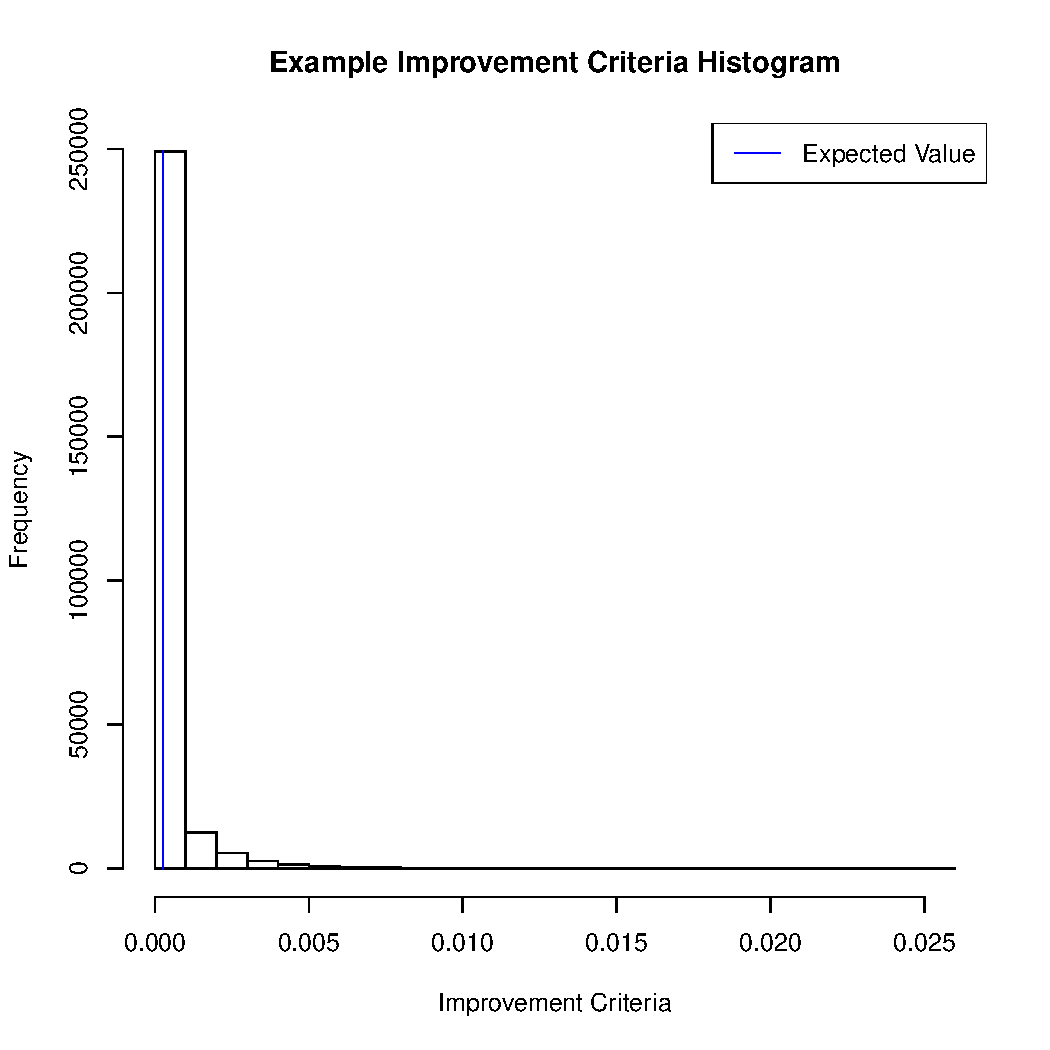
\includegraphics[width=0.5\textwidth]{./figures/exampleIHist.pdf}
% 	\end{center}
% 	\vspace{-0.85cm}
% 	\caption{An example $\ix$ sample histogram, demonstrating the extreme right skew. Additionally, $\Eix$ is shown in blue.}
% 	\label{IxEX}
% 	\end{wrapfigure}
% 	%
% 	%
% 
% 	%
% 	The second major concern brought about by the application of SPC on EI is the distribution of $\ix$.
% 	%
% 	Upon investigation of this distribution it is quickly clear that $\ix$ typically follows a strongly right skewed distribution, due to the non-negative construction of the $\ix$ criterion.
% 	%
% 	This is not a fatal property of the distribution of $\ix$ in terms of the central limit theorem (CLT), although it does yield nearly worst case asymptotics in terms of the convergence of the sampling distribution to normality.
% 	%sampling method longer 
% 	A simple solution for getting more asymptotic results could include increasing the sample size of the draws of $\ix$.
% 	%
% 	However it is important to consider that by the nature of MCMC implementation of models like Model \ref{gpModel}, increasing the number of samples of $\ix$ entails taking more samples of every single parameter in the model.
% 	%
% 	Increasing the sample size of $\ix$ is a perfectly valid solution to this problem, if computation memory is of no concern, but it is not a particularly robust and satisfying solution.
% 	%
% 	Additionally, since the $\ix$ criterion is naturally bounded at 0, an unfettered normal distribution will always struggle to model the EI criterion since the normal distribution will never respect its boundary conditions.
% 	%
% 	Thus, modeling these data so as to find appropriate transformations to improve their asymptotics, and better model the boundary conditions of the problem, is a worthwhile consideration. 
% 	
% 	%
% 	%
% 	
% 	%
% 	In the following sections I address each of these concerns in turn. 
% 	%
% 	As I address each issue, I modify my method for tracking the information contained in the EI criterion so as to robustly identify convergence as inspired by SPC.
% 
% 	%\clearpage
% 	%
% 	%
% 	\subsection{Improved Normality}
% 	%
% 	%
% 	
% 	%
% 	%
% 	\begin{wrapfigure}{l}{0.5\textwidth}
% 	\vspace{-1.1cm}
% 	\begin{center}
% 	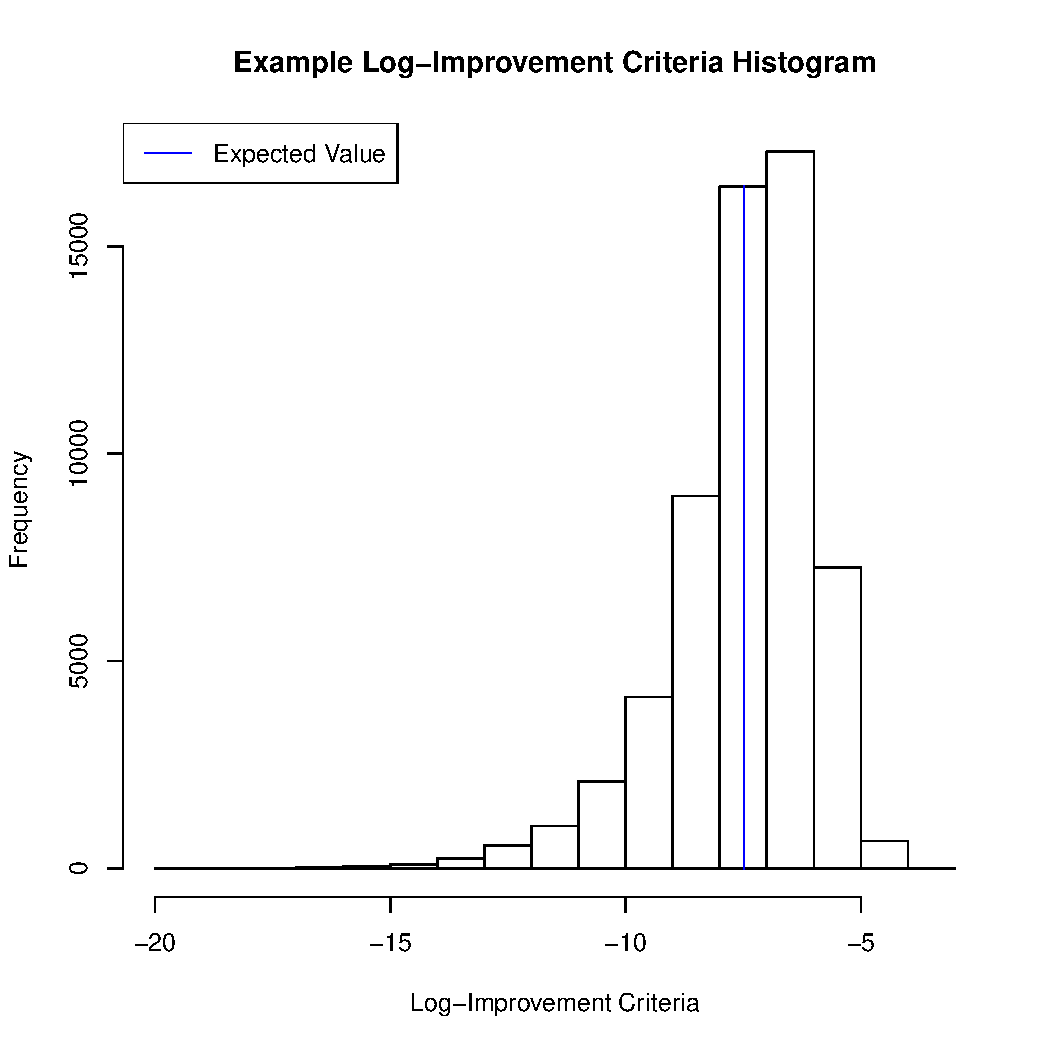
\includegraphics[width=0.5\textwidth]{./figures/exampleLogIHist.pdf}
% 	\end{center}
% 	\vspace{-0.85cm}
% 	\caption{An example $\log\ix$ sample histogram, demonstrating improved skew. Additionally, $\E{\log\ix}$ is shown in blue.}
% 	\label{logIxEX}
% 	\end{wrapfigure}
% 	%
% 	%
% 	
% 	%
% 	For the sake of improving the asymptotic convergence of the EI sampling distribution to normality it is of much desire to transform the distribution of $\ix$ so as to be less skewed.
% 	% of the form seen in figure \cite{IxEX}
% 	A simple and often effective transformation for getting skewed distributions to more resemble normality is a simple $\log$ transformation of the data.
% 	% 
% 	In this case simply log transforming the MCMC samples of the $\ix$ criterion is not always possible.
% 	%
% 	By the definition of the $\ix$ criterion, an $\ix$ sample can at its lowest take a value of 0; see Eq. (\ref{ix}).
% 	%
% 	MCMC samples that explore $\ix$ values as low as 0 will render the $\log$ function useless, as $\log$ is undefined for values $\le 0$.
% 	%
% 	Thus rather than actually transforming the data in this way, I propose modeling these samples with a log-normal distribution.
% 	
% 	%
% 	Recall that if a random variable $X\sim Log$-$N(\mu, \sigma^2)$, then another random variable $Y=\log(X)$ is distributed $Y\sim N(\mu, \sigma^2)$.
% 	%
% 	Furthermore, if $m$ and $v$ are, respectively, the mean and variance of a log-normal sample, then the mean, $\mu$, and variance, $\sigma^2$, of the associated normal distribution are given by the following relation,
% 	%
% 	\begin{eqnarray}
% 	\mu = \ln\left( \frac{m^2}{\sqrt{v+m^2}} \right) &~&  \sigma^2 = \ln\bigg( 1+ \frac{v}{m^2} \bigg).
% 	\label{lnRelate}
% 	\end{eqnarray}
% 	%
% 	Using this relation we do not need to transform any of the $\ix$ samples; we can instead jump straight to the mean of the samples that would have resulted from transforming these $\ix$ samples.
% 	%
% 	That is to say, by using relation \ref{lnRelate} we immediately get a value for $\E{\log\ix}$ without actually taking the log of $\ix$ samples.
% 	%rather than
% 	Considering the distribution of $\log\ix$, seen in figure \ref{logIxEX}, the asymptotics ensuring the normality of the distribution of $\E{\log\ix}$ as compared with that of $\E{\ix}$ are far favorable. % the distribution of  are far favorable to those present necessary for the CLT will be are must more  to work its magic will be ever in our favor through considering the $\E{\log\ix}$ as compared with the standard EI criteria.
% 	
% 	%\clearpage
% 	%
% 	%
% 	\subsection{Exponentially Weighted Moving Average}
% 	%
% 	%
% 	
% 	%{\color{red}EWMA (time series concepts) for added robustness }
% 	%
% 	In general moving average methods use the idea of a rolling average to smooth data that arrive as a series. % techniques for smoothing data that arrive as a series. %, just as is the case for EI values in our optimization routine.
% 	%weighted I not only want to smooth the data, but the calculation of
% 	EWMA methods achieve this smoothing by assigning exponentially decreasing weights to successive points in a rolling average among all of the points of a series. 
% 	%so as to focus the attention of the moving average on recent 
% 	%For application of EWMA on EI progression the smoothing behavior since the EI values can display I am really interested in weighting the values such that more recently observed values are more heavily considered in the moving average.
% 	%
% 	%Exponentially Weighted Moving Averages (EWMA) precisely achieves this goal by assigning exponentially decreasing weights to each point in the series.
% 	%moving
% 	This disproportionately focuses the attention of the moving average on recent information (i.e. the most relevant information in this case), while still smoothing the overall series progression with at least some memory of past values. % giving some weight some memory.  
% 	%%our wild adosecence.focusing our attention on the most relevant, recent, information an display incensed variability and a decreasing trending pattern
% 	These properties of the EWMA have shown to provide a robust solution for tracking the progression of means that are subject to subtle drifting processes \cite{adaptEWMA}, such as one might expect to see in convergence.
% 	% %
% 	% For application of EWMA on EI progression
% 	% Together these properties of the EWMA have the effect of focusing provide a good candidate for monitoring the convergence of EI.
% 	% %
% 	% Since after its initial naive fluctuations, the EI values tend to subtly shift from the early wild fluctuations of pre-convergence   
% 	% since often EI values tend to slowly  as one might expect for the behavior of convergence.
% 
% 	
% 	%
% 	
% 	%the exponentially decreasing weights of tracking the EI values via EWMA in reverse order has the overall effect of
% 	Since early $\E{\log\ix}$ values generally behave differently than later values, I use the EWMA procedure to track the progression of $\E{\log\ix}$ values in reverse order.
% 	%current 
% 	This has the effect of forgiving the wild fluctuations of early inexperienced explorations and highlighting the most recent experiences with $f$. %current values of EI.
% 	%
% 	Furthermore, the exponentially decreasing weights are well suited for monitoring convergence in this case because they have the ability to smooth out the initial EI fluctuations, while still having the resolution to pick out the subtle shifts inherent to the convergence process.
% 	%since after the initial period of naive fluctuations the EI progression tends to subtly slide into convergence, the ability of EWMA to smooth out the initial fluctuations while still picking up on the subtle shifts inherent to convergence makes EWMA a good method for identifying convergence in this case. 
% 	%
% 	Further dynamics of EWMA are well explained by Box et al. \cite{boxBook}; additionally EWMA charts, among other common control charts, can easily be implemented in R by using the R package \verb|qcc| \cite{qccPack}.
% 
% 	%
% 	%
% 	
% 	%
% 	If $Y_i$ is the current value of $\E{\log\ix}$, and $Z_i$ is the EWMA statistic associated with this current value, then the initial value $Z_0$ is set to $Y_0$ and for $i>0$ the EWMA statistic is expressed as,
% 	%
% 	\begin{equation}
% 	Z_i=\lambda Y_i+(1-\lambda)Z_{i-1}.
% 	\label{ewmaStat}
% 	\end{equation}
% 	%
% 	Above, $\lambda$ is a parameter that defines the weight $\left( \text{i.e. }0<\lambda\le1\right)$ assigned to the most recent observation, $Y_i$.
% 	%Eq. (\ref{ewmaStat})
% 	The recursive expression of the statistic ensures that all subsequent weights geometrically decrease as moving back through the series.
% 	
% 	%
% 	%
% 	
% 	%
% 	Typically values of $\lambda$ range from $0.1\le\lambda\le0.3$, with a default value of $\lambda=0.2$, as described by Box et al. \cite{boxBook}.
% 	%
% 	Additionally Box et al. explains how to estimate a $\hat\lambda$ so as to minimize sum of squared deviation ($S_\lambda$) of the resulting EWMA series. %  data specific $\hat\lambda$ value by minimizing the sum of squared deviations with respect to $\lambda$. % , thus tailored for each particular data set.
% 	%the more quickly
% 	In general large values of $\lambda$ assign more weight to recently observed values, and thus past observations effect the moving average less. %  on the moving average quickly forgets about past observations.
% 	%
% 	Conversely, small values of $\lambda$ assign less weight to recent observations, and thus small values of $\lambda$ provide more smoothing across the effects of past observations. 
% 	%provide better sensitivity $\E{\log\ix}$
% 	Hence larger values of $\lambda$ tend to be better suited for dealing with large shifts, and small values of $\lambda$ are more sensitive to small shifts.
% 	%
% 	Often it is the case with EWMA that the best choice of $\lambda$ is based on ``expert opinions'' related to the underlying data generating process.
% 	%the choice of an appropriate $\lambda$ requires an
% 	For identifying convergence, ``expert opinions'' come in the form of an in-depth understanding of how EI values behave relative to the specific search phenomena related to the expected behavior of $f$.
% 	%Hence larger values of $\lambda$ tend to be better suited for dealing with the large EI shifts associated with uncertain mean predictive surfaces.
% 	%In contrast, small values of $\lambda$ are more sensitive to small EI shifts, and thus are well suited for identifying convergence when the 
% 	
% 	%
% 	%
% 	
% 	%how the plot In order to identify convergence
% 	For identifying convergence it is also important to define the control limits on the statistic seen in Eq. (\ref{ewmaStat}).
% 	%
% 	Again, this amounts to considering an interval on the sampling distribution of interest.
% 	%, under the assumptions that the $Y_i$ arrive as $i.i.d.$ samples
% 	In this case we are interested in the sampling distribution of the $Z_i$, if the $Y_i$ are $i.i.d.$ then Lucas and Saccucci \cite{ewmaPaper}  show that we can write $\sigma^2_{Z_i}$ in terms of $\sigma^2_{Y}$. %, Lucas and Saccucci \cite{ewmaPaper}  show,
% 	%
% 	\begin{equation}
% 	\sigma^2_{Z_i} = \sigma^2_{Y}\left(\frac{\lambda}{2-\lambda}\right)\left[1-(1-\lambda^{2i})\right]
% 	\end{equation}
% 	%\substack{i.i.d.\\\sim}
% 	Thus if the $Y_i \stackrel{i.i.d.}{\sim} N\left(\mu, \frac{\sigma^2}{n}\right)$ the sampling distribution for $Z_i$ is $Z_i \sim N\left(\mu, \sigma^2_{Z_i}\right)$.
% 	%
% 	Furthermore if we choose a confidence level through a choice of the constant $c$, the control limits based on this sampling distribution follow on the next page.
% 	
% 	%
% 	\begin{figure}
% 	\vspace{-1cm}
% 	\begin{eqnarray}
% 	\text{CL}_i &=& \mu \pm c \sigma_{Z_i}\nonumber\\
% 	&=&  \mu \pm c ~ \frac{\sigma}{\sqrt{n}}~\sqrt{\left(\frac{\lambda}{2-\lambda}\right)\left[1-(1-\lambda^{2i})\right]}
% 	\end{eqnarray}
% 	\end{figure}
% 	%
% 	
% 	$~$\\\\
% 	Notice that since $\sigma^2_{Z_i}$ has a dependence on $i$, the control limits do as well.
% 	%the focusing effect of EWMA. % this focusing effect.
% 	Looking back through the series brings us away from the focus of the moving average, at $i$, and thus the control limits widen when traversing backwards through the series resulting directly from the geometrically decreasing weights.  
% 	%
% 	
% 	%
% 	%
% 	
% 	%
% 	At this point it is necessary to take a step back from the modeling details and motivate the use of such models on the real $\E{\log\ix}$ behavior.
% 	%
% 	At first glance it is not clear that the $Y_i$ are in fact $i.i.d$. % throughout the entire progression of values. % \stackrel{i.i.d.}{\sim} N\left(\mu, \frac{\sigma^2}{n}\right)$.
% 	% thus making the $i.i.d.$ assumption appropriate.
% 	Indeed the early iterations of the process certainly do not display $i.i.d.$ looking $Y_i$ values.
% 	%
% 	However once the process proceeds far enough, the $Y_i$ enter a state of control; thus for the values that are in control, the $i.i.d.$ assumption is very reasonable.
% 	%identifies the
% 	The fact that the pre-convergence $Y_i$ do not necessarily demonstrate control may in large part have to do with their lack of $i.i.d.$ness, and thus identifying control in this way validates the appropriateness of this model by identifying control. % in which the notion of $i.i.d.$ness is implied.
% 	%
% 	That is to say, in this application the concept of $i.i.d$ samples serves as part of the check for control; realizing control validates the assumption of $i.i.d.$ samples and vice versa.
% 	%be due to their identification as  prior to reaching control do not require  Prior to reaching control 
% 	%The notion of control implies some Inherent to the idea of control is the idea that the process is $i.i.d.$ 
% 	%
% 	%The particular interest for the accuracy of this model surrounds the identification of convergence, and since the $Y_i$ presumably enter a state of control at convergence and convergence requires a reasonable $i.i.d$ assumption the idea is that when it really matters   
% 	%and furthermore, the $\ix$ criteria suffers from a strong right skew.
% 	
% 	%
% 	%
% 	
% 	%
% 	Another detail worth further recognition, is the asymptotics on which all of the this logic is built.
% 	%Let us not forget that, e
% 	Even after log transformation of the $\Eix$ criterion, $\E{\log\ix}$ is still only asymptotically normal.
% 	%
% 	Even though the distribution of $\E{\log\ix}$ is likely to be quite normal, via the CLT, it is still worth mentioning that any non-normality left in the model is left for EWMA's own robustness to cope with. 
% 	%In section 2.2 I address a modeling consideration that should drastically improve the assumption of normality on the $Y_i$. % %in this case.
% 	%
% 	Furthermore, constructing a robust model for identifying convergence is of primary concern, especially considering the many varied conditions this model must perform under.
% 	%
% 	In considerations of this type, Box et al. \cite{boxBook} argues that EWMA is a robust and parsimonious solution in many cases, especially with respect to disputes in the distribution and stationarity of the $Y_i$.
% 	% and provide accurate results in many situations
% 	Thus the EWMA logic should provide the sturdy and robust framework necessary for dealing with data of \mbox{this type.}  
% 	
% 	%
% 	%
% 	\subsection{The Control Window}
% 	%
% 	%
% 	
% 	%
% 	%However, there are some issues in the application of a naive
% 	%
% 	%One additional feature is necessary to adapt to typical SPC philosophy so as to identify convergence.
% 	%
% 	Typically in SPC some initial number of samples are gathered and deeply investigated to establish an initial standard for control that is not wildly off-base.
% 	%
% 	Investigation in this setting amounts to careful analysis of the conditions related to points that fall beyond the control limits; often with the intention of attributing some deterministic reason for the lack of control.
% 	%
% 	Observations investigated in this way are often discarded from the calculation of initial control limits because they are found not to represent the desired state of control, and thus through their exclusion the standard for control is elevated.
% 	
% 	% 
% 	In the setting of optimization it is not desirable to study each pass of our routine so carefully, and often such analysis would not be meaningful.
% 	%
% 	However, for the sake of keeping in the spirit of SPC, as well as other practicalities, I offer a compromise that frames the setting for which convergence is to be identified.
% 	%
% 	I propose the idea of a sliding window of fixed size, $w$, that I call the {\it control window}.
% 	%is to be  all be the sole provider of information for the calculation of control limits.in the calculation of
% 	The idea being, only information from the $w$ points currently residing inside the control window is used to calculate the control limits, but the EWMA statistic is still computed for all values as before.
% 	%contribute information toward
% 	%The EWMA statistic shall be computed for all values, but only a set number, say $w$ of the values, shall reside inside the control window at any given time, and thus only these $w$ values are included in the construction of control limits.
% 	%
% 	%Since 
% 	%, so as to fill the control window
% 	Initially, I allow the algorithm to fill the control window, by collecting $w$ observations of $f$.
% 	%;
% 	As new observations of $f$ arrive, the oldest value is removed from the control window, thus allowing for the inclusion of a new value.
% 	%\singlespacing
% 	This offers an automated way of basing the standard for convergence only on the most updated and relevant information.
% 	%
% 	%Furthermore since at convergence we only require control inside the control window, basing the control limits solely on information for the  validated the necessary $i.i.d$ assumption in constructing the control limits.
% 	
% 	%
% 	%
% 	
% 	%The size of this window is left up to the discretion of user,.
% 	The size, $w$, of the control window is important for correctly identifying convergence.
% 	%
% 	Because $w$ may vary from problem to problem it is ultimately left as a tuning parameter of the system.
% 	%
% 	Choosing the correct value of $w$ presents an interesting decision problem since underestimating the size of the control window may lead to premature convergence, but if $w$ is too large, we compute unnecessary objective function evaluations.
% 	%It is t
% 	Thus it may be important to consider these two opposing forces when choosing an appropriate value for $w$.
% 	%
% 	I recommend conservatively large values for $w$ because I regard premature convergence to be a greater problem than extraneous function evaluations.
% 	%
% 	As a default value $w=30$ has provided me a reasonable starting point for further analysis.
% 	%
% 	I have found that choosing $w$ based on the value of $\lambda$ seems to be an efficient way of tuning $w$.
% 	%
% 	As a general trend, the larger the value of $\lambda$, the more fluctuation present in the EWMA statistic.
% 	% the fluctuations in the EWMA statistic. %Conversely for small $\lambda$, smaller values of $w$ are acceptable. are necessary allow averages over more elements of the  to  average out ; fluctuations 
% 	Thus for good results, large $\lambda$, naturally imply large values of $w$ for an accurate representation of the increased fluctuations of the EWMA statistic in the repeated sampling average.
% 	%due to decreased fluctuations in the EWMA statistic
% 	Conversely for small $\lambda$, smaller values of $w$ are acceptable.
% 
% % 	\clearpage
% 	%
% 	%
% 	\subsection{EWMA Convergence Chart}
% 	%
% 	%
% 	
% 	%
% 	Recall that this work is meant to apply at step 7) of figure \ref{procedure}.
% 	%
% 	Thus, at each iteration we can obtain a new $\E{\log\ix}$ value to track via the EWMA procedure outlined in Section 2.2.
% 	%
% 	If we then apply the control window to this EWMA tracking procedure, interesting rules for identifying convergence naturally arise. 
% 	
% 	%
% 	%
% 	
% 	%triggers an out-of-control state when a $Z_i$ value exceeds the established control limits.
% 	The typical EWMA identifies out-of-control observations  by simply identifying which $Z_i$ values exceed the established control limits. This may be adequate for a check of simple
% 
% 	%
% 	%
% 	\begin{wrapfigure}{l}{0.5\textwidth}
% 	\vspace{-1.1cm}
% 	\begin{center}
% 	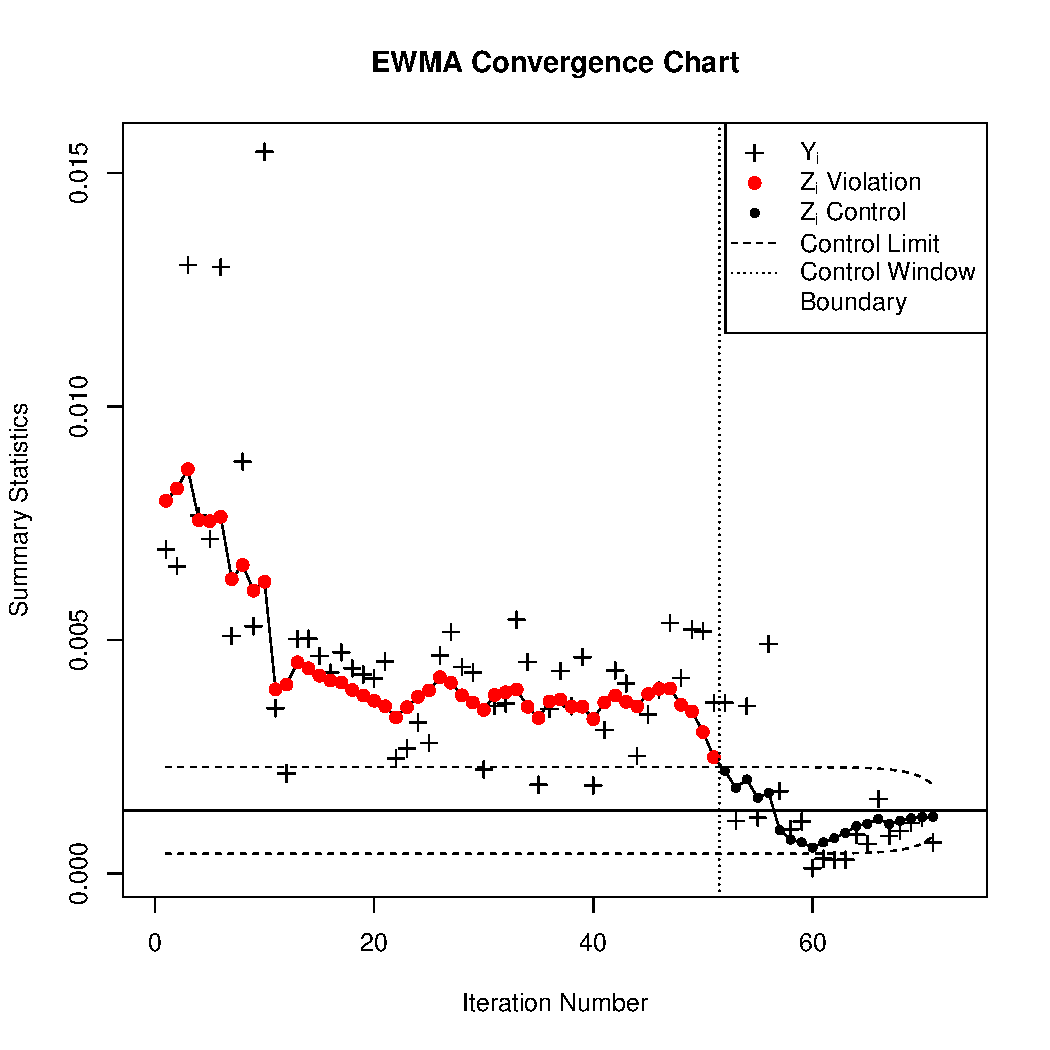
\includegraphics[width=0.47\textwidth]{./figures/exampleEWMA.pdf}
% 	\end{center}
% 	\vspace{-0.85cm}
% 	\caption{An example EWMA convergence chart based on the fabricated EI progression in figure \ref{EIxEX}. This chart is converged.}%has identified convergence. }
% 	\label{EXconverge}
% 	\end{wrapfigure}
% 	%
% 	%
% 
% 	%This may be adequate for a check of simple
% 	\noindent control, but is not a stringent enough standard for determining convergence.
% 	%converged state to be in control
% 	In identifying convergence we not only desire that the converged state has reached a state of control, but we also desire a state of control that indicates significantly lower expectations for finding new minima in the future.
% 	%
% 	This suggest a dual use of the the control window in suggesting convergence.
% 	%% that they define.
% 	Firstly, I require that all $Z_i$ values inside the control window fall within the control limits. 
% 	%the past (i.e.. outside the control window)
% 	Secondly, since we wish to indicate a move from the initial pre-converged state of the system, I require at least one point from beyond the control window to fall outside the defined control limits.
% 	%the intersection of
% 	A set of $Z_i$ satisfying both of these conditions indicate the desired state of convergence.
% 	%
% 	Satisfying only one of these conditions indicates insufficient exploration of the objective landscape and thus further iterations of procedure \ref{procedure} are required.
% 	
% 	%is a type of moving control. , thus sliding
% 	Together these rules capture the notion that the process of convergence is a slide from a pre-convergence state, into a converged state of control. 
% 	%recent values of $Z_i$ (i.e.
% 	In the converged state, $Z_i$ values in the control window (i.e. recent values) indicate control in the classical sense.
% 	% so as to identify convergence.it provides a way to express the idea of moving control,Additionally, s
% 	Since the control window partitions the $Z_i$ into new and old values, the control window provides a mechanism for identifying when control has shifted into a state of control that has moved sufficiently from the initial pre-convergence state.
% 	%
% 	These added considerations for the behavior of current $Z_i$ values, relative to old observations, differentiate the classical notion of control charts from what I call a convergence chart.  
% 	
% 	
% %
% %
% \section{Examples}
% %
% %
% 
% %of monitoring convergence via the above described EWMA convergence chart.
% In this section I provide a series of test function examples, as well as a case study demonstrating the use of the EWMA convergence chart for monitoring convergence.
% %a strategy - or - strategies
% The test function examples are meant to highlight strategies for tuning $\lambda$ and $w$ relative to the observed behavior of $f$, as well as demonstrate various states of convergence with respect to various objective function behaviors.
% %
% Additionally, I consider the Lockwood pump-and-treat case study as a practical example of how the EWMA convergence chart may be used in less tidy optimization problems.
% 	
% 	%\clearpage
% 	%
% 	%
% 	\subsection{Rosenbrock}
% 	%
% 	%
% 	
% 	\begin{figure}[!h]%{l}{1.\textwidth}
% 	\centering
% 	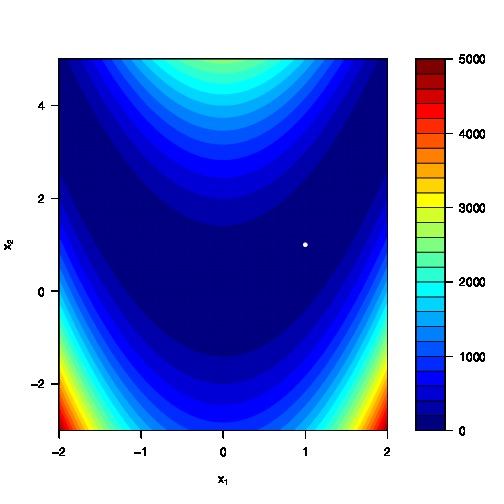
\includegraphics[width=0.49\textwidth]{./figures/roseContour.jpg}
% 	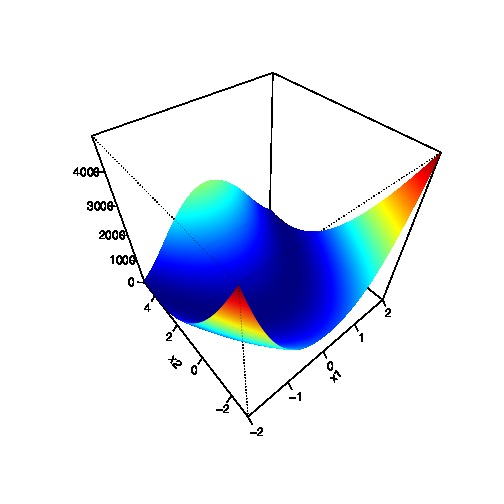
\includegraphics[width=0.49\textwidth]{./figures/rosePersp.jpg}
% 	\begin{eqnarray}
% 	f(x_1, x_2) &=& 100\left(x_2-x_1^2\right)^2 + (1-x_1)^2 \\
% 	\text{Minimum}&:& f(1, 1)=0\nonumber
% 	\end{eqnarray}	
% 	\end{figure}
% 	
% 	%banana-shaped
% 	The Rosenbrock function \cite{rosePaper} is a classic optimization benchmark, and thus it is only fitting to begin with an analysis of its long and narrow, flat parabolic valley.
% 	%
% 	Exploring the banana-shaped valley is an exercise in self control, as the flat valley floor seems to endlessly meander around the curve of the banana with relatively little descent as compared with the steep $4^{th}$ order polynomial valley walls.   
% 	%% of the valley.
% 	This stark difference in scale tempts optimization routines to prematurely claim convergence all along the lengthy valley floor. 
% 	%% just above and to the right of the vertex of the parabolic valley.
% 	As indicated above, the true global minimum value is attained jarringly off centered at (1, 1), where the objective value eventually falls to 0. 
% 	
% 	%above pictured % , with of the Rosenbrock function,
% 	For the sake of this analysis I focus on the pictured intervals, in this example I am focusing on Rosenbrock with \mbox{$-2\le x_1\le2$}; \mbox{$-3\le x_2\le5$}.
% 	%(i.e. \mbox{$-2\le x_1\le2$} and \mbox{$-3\le x_2\le5$}) %% The pictured interval% we ... the model
% 	This interval subjects the surrogate model to the flat valley floor, but since we start optimization with a naively chosen $\bm{X}$,  initially the model is forced to make some consideration of the steep valley walls.
% 	
% 	%
% 	%surrogate model of the surrogate modeling procedure.
% 	\begin{wrapfigure}{l}{0.5\textwidth}
% 	\vspace{-1.1cm}
% 	\hspace{-1cm}
% 	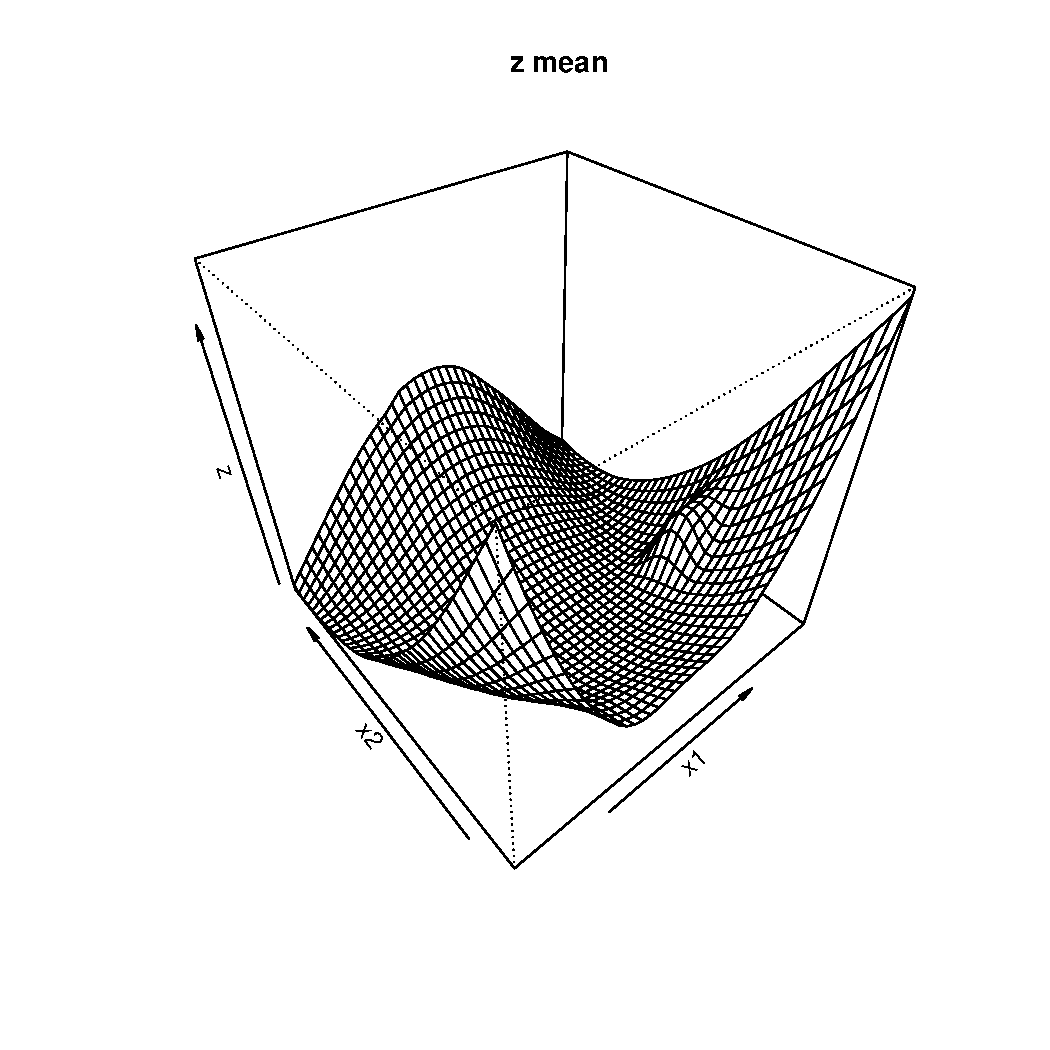
\includegraphics[width=0.6\textwidth]{./figures/gpMeanRosegpPic.pdf}
% 	\vspace{-2.5cm}
% 	\caption{The GP mean predictive surface of the Rosenbrock function after 70 iterations. }
% 	\label{roseGP}
% 	\end{wrapfigure}
% 	%
% 	%
% 	%
% 	\noindent
% 	As optimization, proceeds only the maximum EI candidate location is added to $\bm{X}$, and thus for the sake of optimization no time is wasted searching for a minimum in the steep walls. % we don't  
% 	%we gather more and more 
% 	Furthermore, since the maximum EI candidate location typically falls somewhere in the valley floor, more and more points from inside the valley are gathered.
% 	%surrounding valley walls
% 	This forms a very good model for what the true shape of the Rosenbrock function looks like inside this valley, but gives only the necessary impression of the surrounding walls needed to identify that they do not contain minima, as seen in Figure (\ref{roseGP}).
% 	%
% 	
% 	%
% 	%
% 	
% 	%with respect to GP surrogate model optimization. example demonstrates a very typical case typical case  for identifying convergence.
% 	Since the Rosenbrock function is not highly multimodal and does not contain any hard to discover features, it provides an example of the kind of function that will provide the default EI behavior.  
% 	%
% 	%Thus this represents a default setting for choosing values of the tuning parameters $\lambda$ and $w$.
% 	%
% 	The basic strategy for tuning $\lambda$ and $w$ starts by first choosing a value for $\lambda$, to remove a degree of freedom from the system. %, by choosing a value for $\lambda$.
% 	%
% 	Since Rosenbrock provides an example of default convergence behavior, the default $\lambda$ value is appropriate, $\lambda=0.2$.
% 	%easily
% 	After choosing $\lambda$, the choice of $w$ can be made based on the chosen value of $\lambda$.
% 	%
% 	Again since $\lambda$ was chosen in accordance with the default value, the default value of $w=30$ is also appropriate here.
% 
% 	%identifying convergence 
% 	Recall that for constructing an EWMA convergence chart it is necessary to first fill the control window so as to establish some initial opinion of the searching process.
% 	%
% 	Figure (\ref{roseEWMAStart}, {\it left}) shows this initial, pre-convergence state, for the Rosenbrock function as described thus far.
% 	%\clearpage
% 	%
% 	%
% 	\begin{wrapfigure}{l}{0.5\textwidth}
% 	%\hspace{-1cm}
% 	\vspace{-0.2cm}
% 	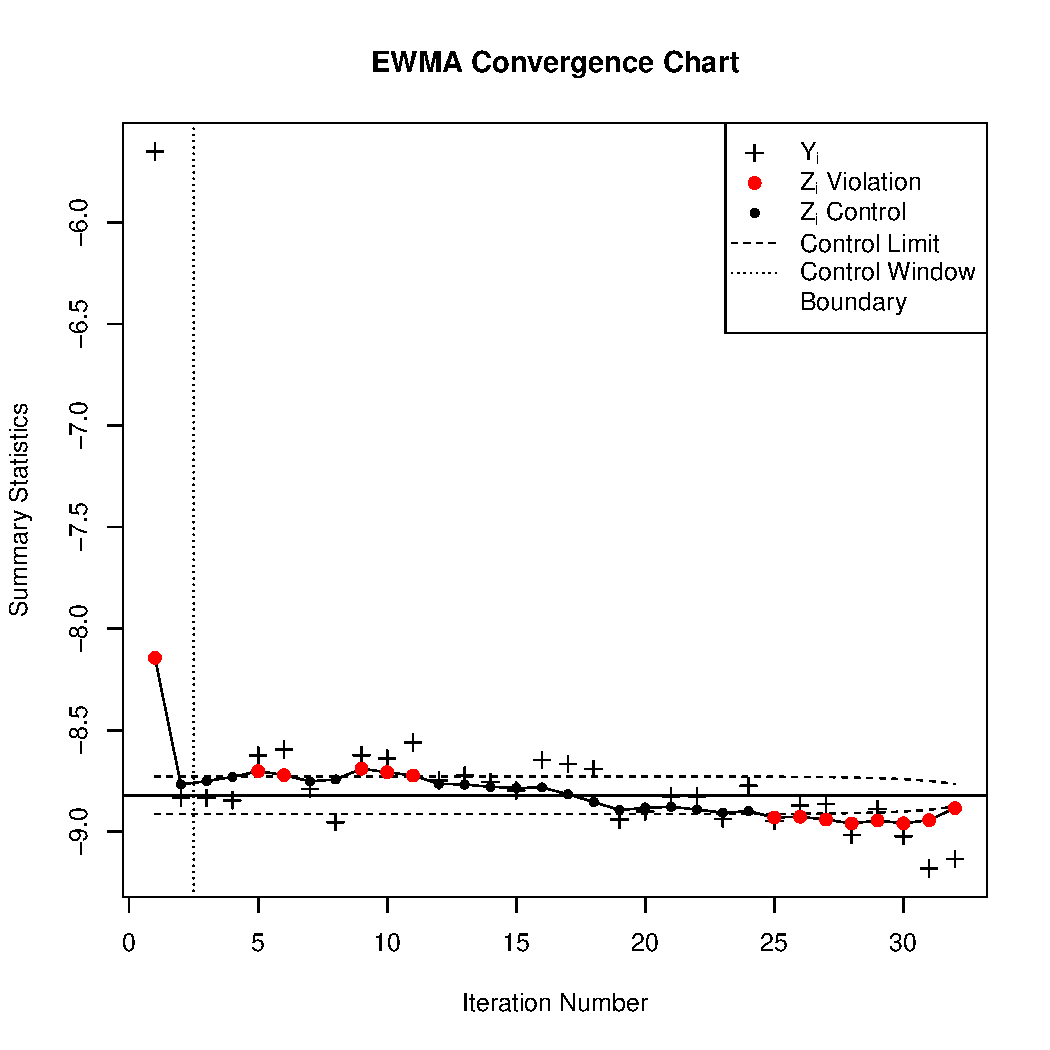
\includegraphics[width=0.245\textwidth]{./figures/ewmaConvChartRoseEasyEasyStart.pdf}
% 	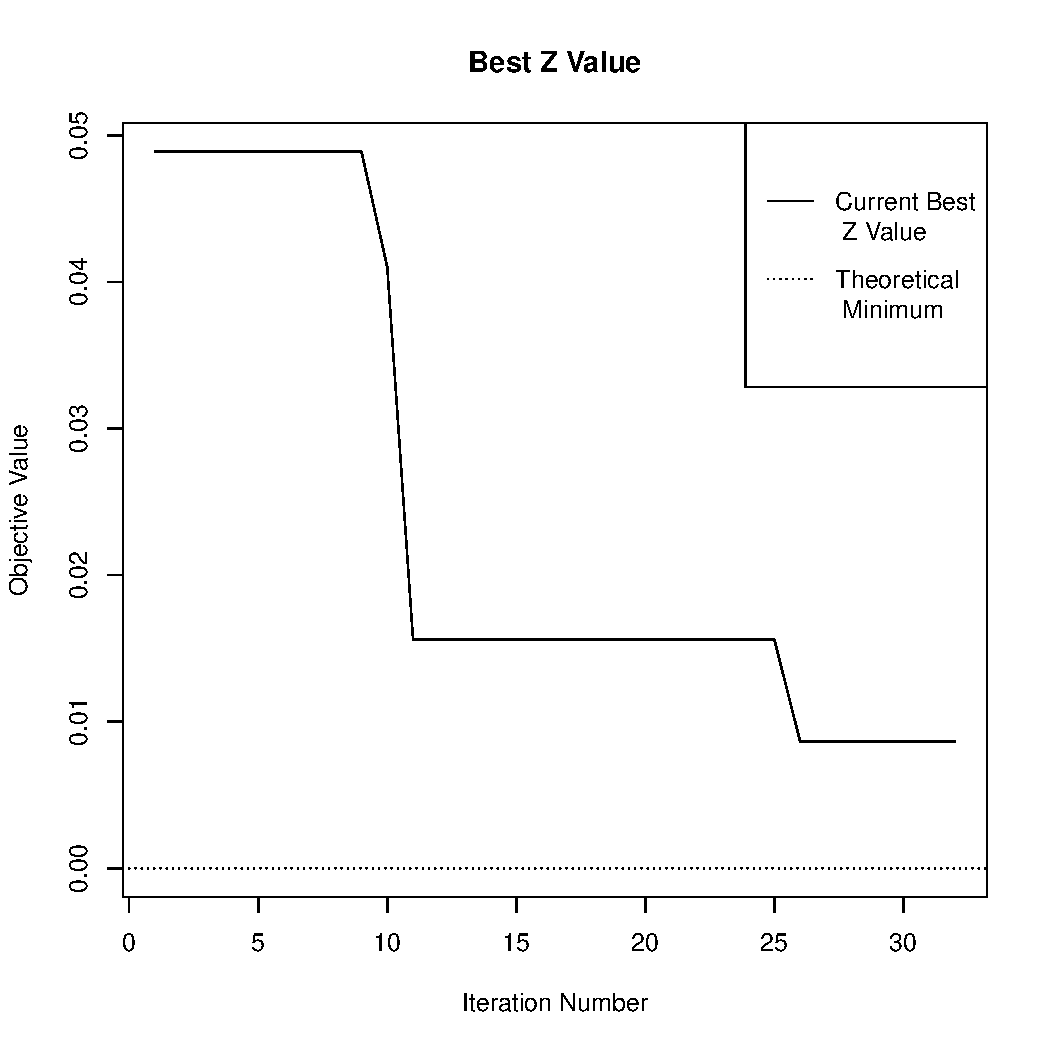
\includegraphics[width=0.245\textwidth]{./figures/bestZRoseEasyEasyStart.pdf}
% 	% for Rosenbrock
% 	\caption{({\it left}) The initial pre-converged state of the EWMA convergence chart. ({\it right}) The cumulative smallest objective function value at each iteration.}
% 	\label{roseEWMAStart}
% 	\end{wrapfigure}
% 	%
% 	%
% 	%
% 	\noindent
% 	The EWMA convergence chart shows an out-of-control state in the control window, with violations of the upper control limit for older values and violations of the lower control limit for more recently observed values.
% 	%
% 	This pattern indicates that the $\E{\log\ix}$ values are still in a steady decreasing state, and more iterations of the optimization procedure are required.
% 	%
% 	As the optimization procedure is allowed to proceed these violations move out of the control window and eventually a set of $\E{\log\ix}$ values fill the control window which do not display any violations inside the control window, as seen in Figure (\ref{roseEWMAEnd}, {\it left}).
% 	%
% 	Furthermore Figure (\ref{roseEWMAEnd}, {\it left}) demonstrates convergence because virtually all of the values beyond the control window violate the upper control limit.
% 	%
% 	
% 	%as optimization proceeds.
% 	As a check of the accuracy of the EWMA convergence chart, the right panels of both \mbox{Figures (\ref{roseEWMAStart}) and (\ref{roseEWMAEnd})} track the smallest objective function evaluation observed. 
% 	%
% 	\begin{wrapfigure}{l}{0.6\textwidth}
% 	%\hspace{-1cm}
% 	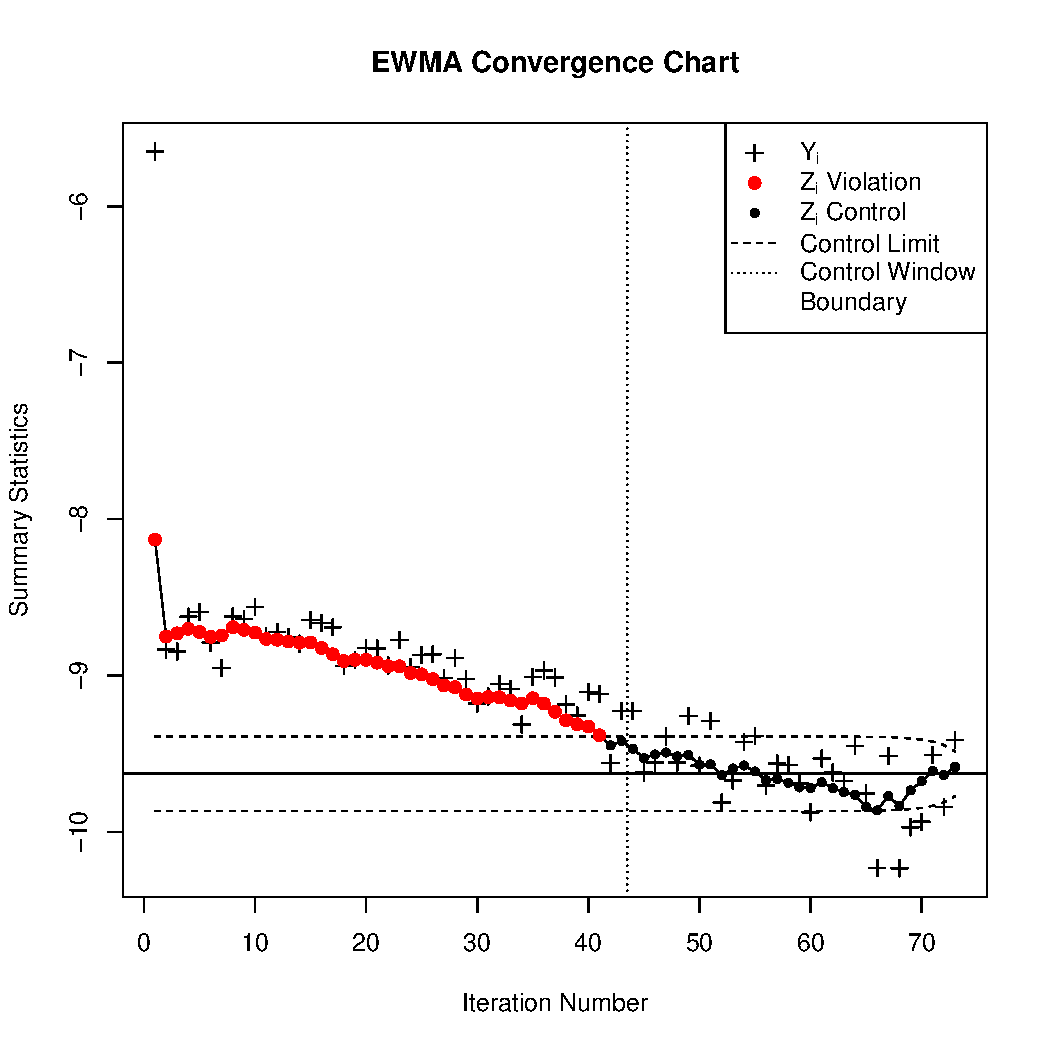
\includegraphics[width=0.245\textwidth]{./figures/ewmaConvChartRoseEasyEasyEnd.pdf}
% 	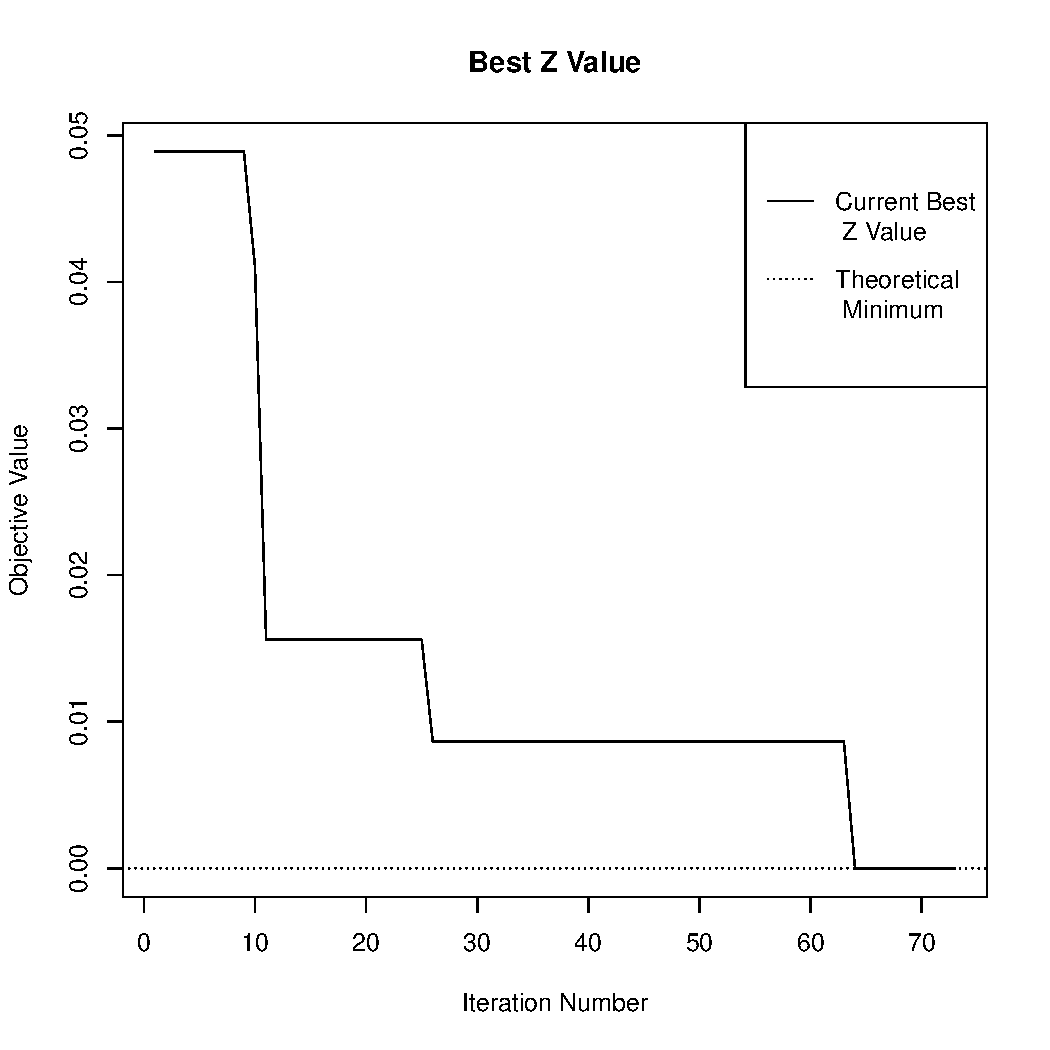
\includegraphics[width=0.245\textwidth]{./figures/bestZRoseEasyEasyEnd.pdf}
% 	% for Rosenbrock
% 	\caption{({\it left}) The converged state of the EWMA convergence chart. ({\it right}) The cumulative smallest objective function value at each iteration.}
% 	\label{roseEWMAEnd}
% 	\end{wrapfigure}
% 	% 
% 	Notice that in Figure (\ref{roseEWMAStart}, {\it right}) the surrogate model appears to have found a sub-optimal location within Rosenbrock's valley, but the EWMA convergence chart does not indicate convergence.
% 	%
% 	In Figure (\ref{roseEWMAEnd}, {\it left}) the EWMA convergence chart does indicate convergence shortly after the surrogate model finds a value that is indistinguishable from Rosenbrock's theoretical minimum value.
% 
% 
% 	%\clearpage
% 	%
% 	%
% 	\subsection{Rastrigin}
% 	%
% 	%
% 	
% 	\begin{figure}[!h]
% 	\centering
% 	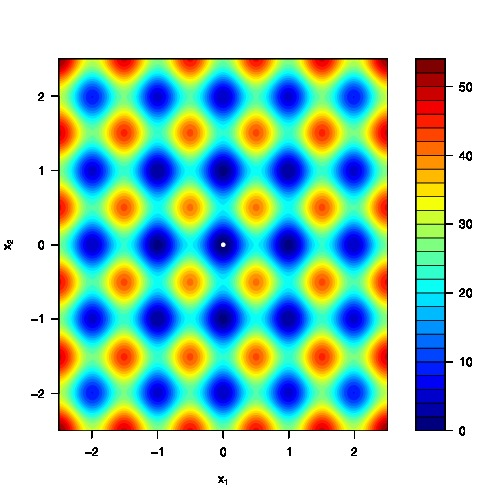
\includegraphics[width=0.49\textwidth]{./figures/rastContour.jpg}
% 	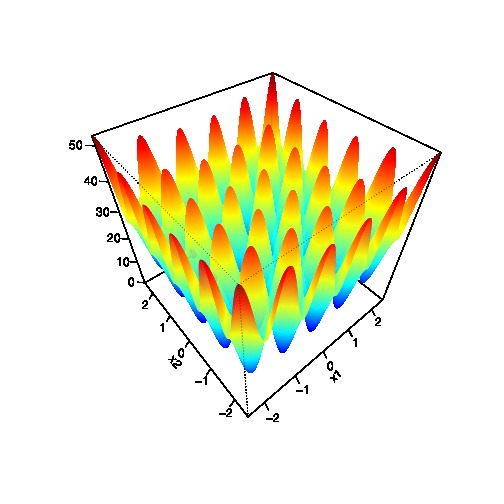
\includegraphics[width=0.49\textwidth]{./figures/rastPersp.jpg}
% 	\vspace{-0.5cm}
% 	\begin{eqnarray}
% 	f(x_1, x_2) &=& \sum_{i=1}^2\left[x_i^2-10\cos(2\pi x_i)\right] + 2(10)\\
% 	\label{rastEq}
% 	\text{Minimum}&:& f(0, 0)=0\nonumber
% 	\end{eqnarray}
% 	\end{figure}
% 	
% 	%\vspace{-0.5cm}
% 	%
% 	The Rastrigin function \cite{rastCite} is a commonly used test function on genetic algorithms; in this setting it offers an interesting example for considering convergence for highly multimodal objective functions.
% 	% located  nadir  lowest point objective 
% 	The global behavior of Rastrigin is dominated by the spherical function, $\sum_i x_i^2$, however Rastrigin has been oscillated by the $\cos(.)$ function, and shifted, so that it achieves a global minimum value of 0 at the lowest point, of its lowest trough at (0, 0).
% 	
% 	%
% 	%
% 	
% 	%
% 	Tuning $\lambda$ and $w$ in this case requires careful consideration of how Rastrigin's many modes effect the exploration process.
% 	%
% 	Again the basic parameter tuning strategy is to first determine an appropriate value for $\lambda$, then tune $w$ conditionally on the expected behavior of the EWMA statistic for the chosen value of $\lambda$.
% 	%
% 	Rastrigin's many modes mean that as the objective landscape is explored, the algorithm will regularly find features indicative of possible new minima. %  of the objective landscape proceeds 
% 	%
% 	Initially this drives up the value of the EI criterion, but as each of these modes are adequately explored, and disregarded, the EI value experiences large downward shifts.
% 	%
% 	To accurately track these large shifts it is required to choose a large value for $\lambda$. 
% 	%
% 	Recall that typical values for $\lambda$ lie in the range $0.1\le\lambda\le0.3$; in this case it is sufficient to simply choose the upper threshold of this typical range, thus $\lambda$ is set to $\lambda=0.3$.
% 	%
% 	Since the increased value for $\lambda$ results in a more actively fluctuating EWMA statistic, the choice of $w$ must reflect this knowledge.
% 	%
% 	In the default case $w=30$, but to account for the increased fluctuations brought about by a larger $\lambda$ value, $w$ is increased to $w=40$. 
% 	
% 	
% 	%upper and lower
% 	As before, the initial EWMA convergence chart, seen in Figure (\ref{rastEWMAStart}, {\it left}), indicates a lack of control, as demonstrated by the violations of the control limits inside the control window.
% 	% of Eq. (\ref{rastEq}).by right panel of
% 	This out-of-control chart indicates that the algorithm has not yet converged, which is confirmed Figure (\ref{rastEWMAStart}, {\it right}), showing that initially the smallest objective value
% 	%
% 	%
% 	\begin{wrapfigure}{l}{0.6\textwidth}
% 	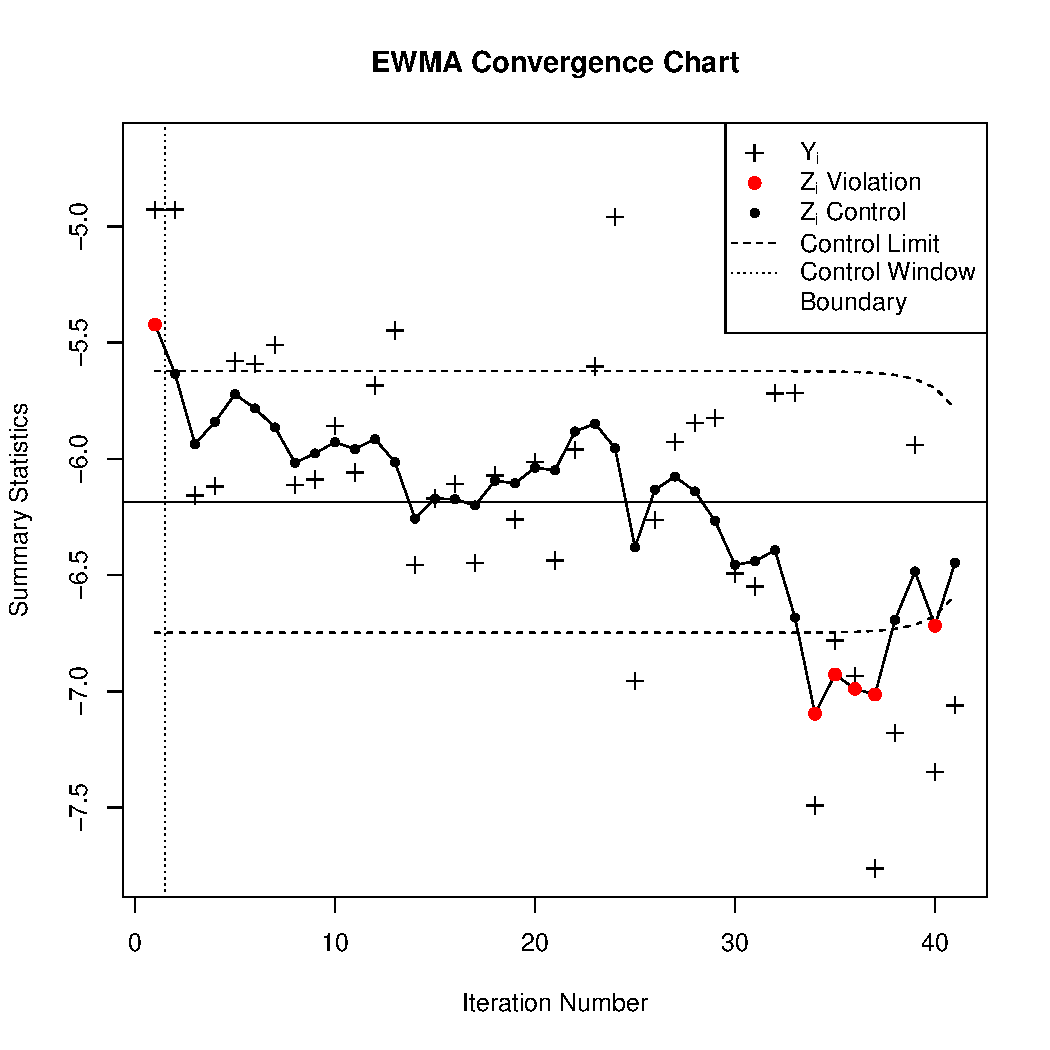
\includegraphics[width=0.245\textwidth]{./figures/ewmaConvChartRastHardStart.pdf}
% 	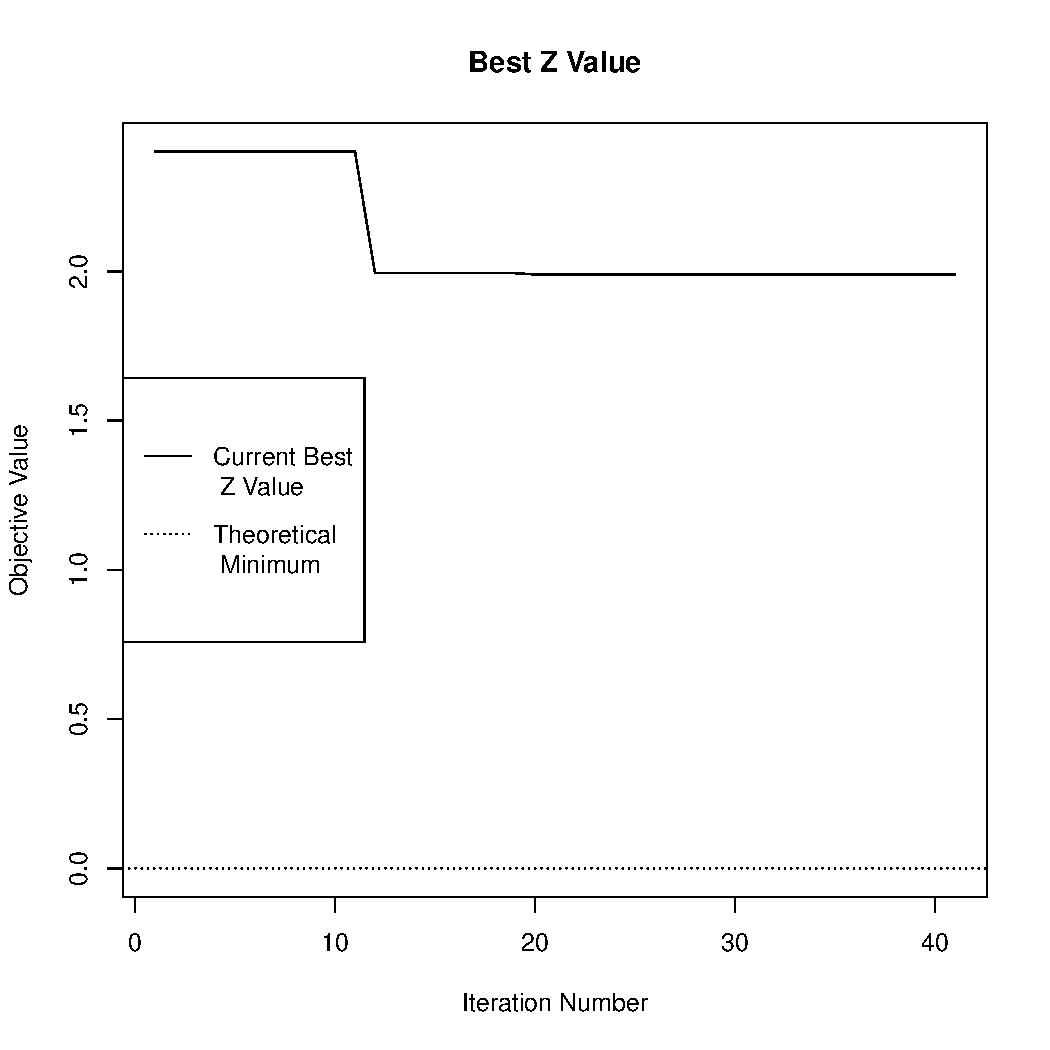
\includegraphics[width=0.245\textwidth]{./figures/bestZRastHardStart.pdf}
% 	\caption{Initial EWMA convergence chart and smallest objective function value. }
% 	\label{rastEWMAStart}
% 	$~$\\
% 	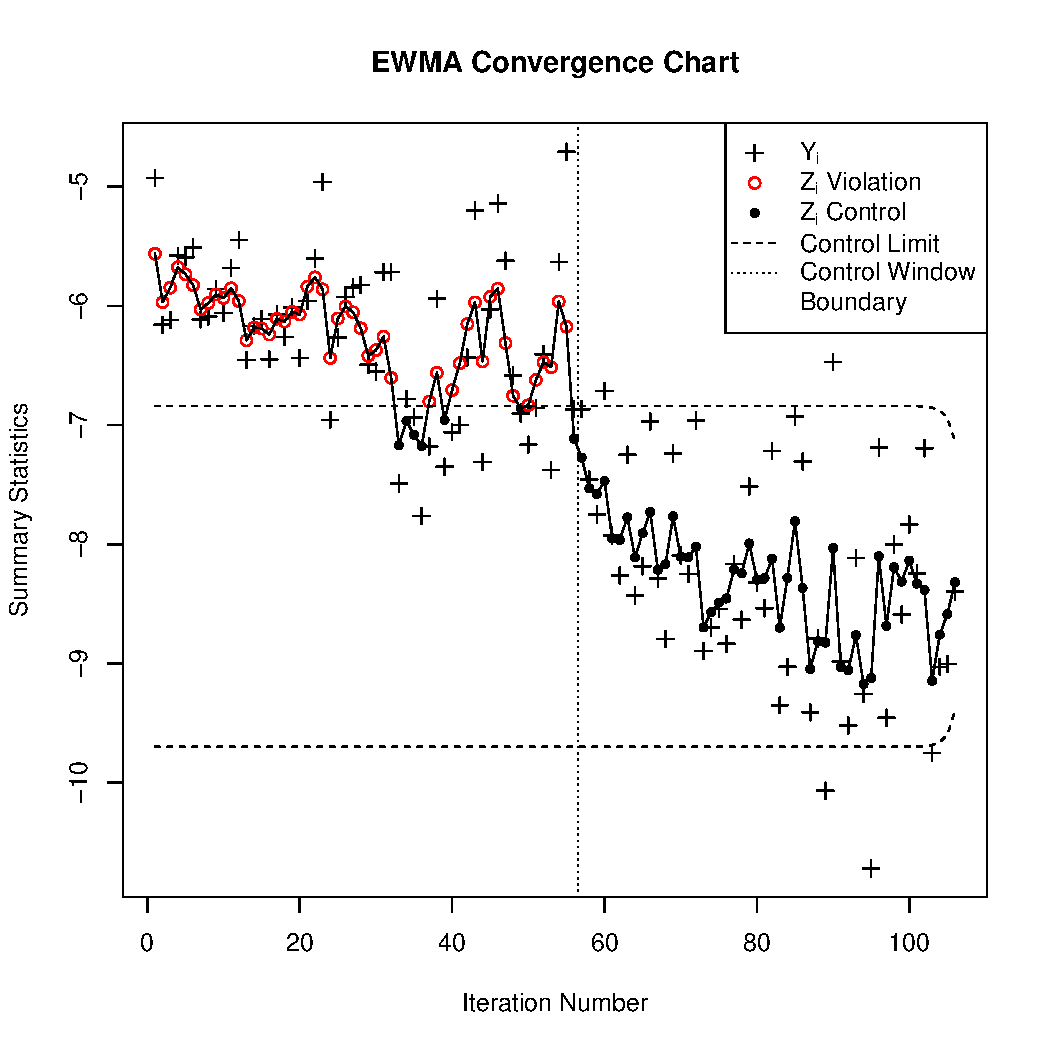
\includegraphics[width=0.245\textwidth]{./figures/ewmaConvChartRastHardEnd.pdf}
% 	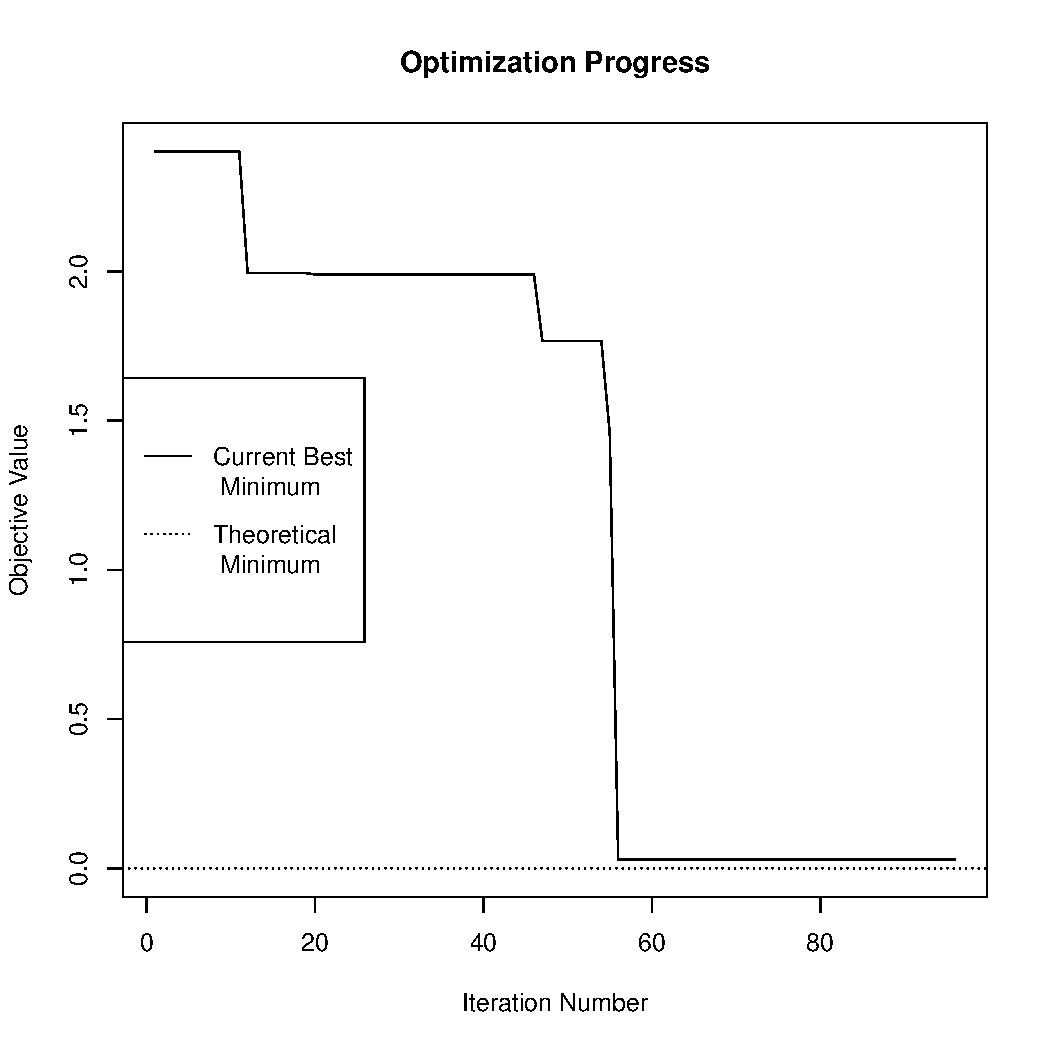
\includegraphics[width=0.245\textwidth]{./figures/bestZRastHardEnd.pdf}
% 	\caption{Final EWMA convergence chart and smallest objective function value. }
% 	\label{rastEWMAEnd}
% 	\end{wrapfigure}
% 	%
% 	%in the initial state
% 	is far from the theoretical minimum.
% 	%the right panel shows that 
% 	Considering Figure (\ref{rastEWMAEnd}, {\it right}), after about 55 iterations the algorithm finds nearly the theoretical minimum, but it takes until about iteration 90 for enough of the large EI values to move out of the control window so that the EWMA control chart can claim convergence.
% 	%
% 	Notice that since the value of $\lambda$ was increased here, the fluctuations in the EWMA statistic have also increased as compared with Figure (\ref{roseEWMAEnd}, {\it left}).
% 	%Smaller values of $w$ would open up here 
% 	The larger value of $w$ is needed to alleviate the possibility of introducing small sample biases, introduced by the increased EWMA fluctuations, in long-run average estimates in computing the control limits.
% 	%
% 	Thus decreasing $w$ here would increase the prevalence of false claims of convergence.
% 	
% 	%\clearpage
% 	%
% 	%
% 	\subsection{Easom}
% 	%
% 	%
% 	
% 	%
% 	%
% 	\begin{figure}[!h]
% 	\centering
% 	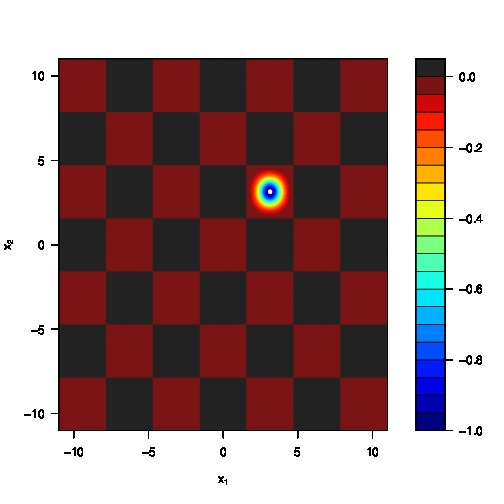
\includegraphics[width=0.49\textwidth]{./figures/easomContour.jpg}
% 	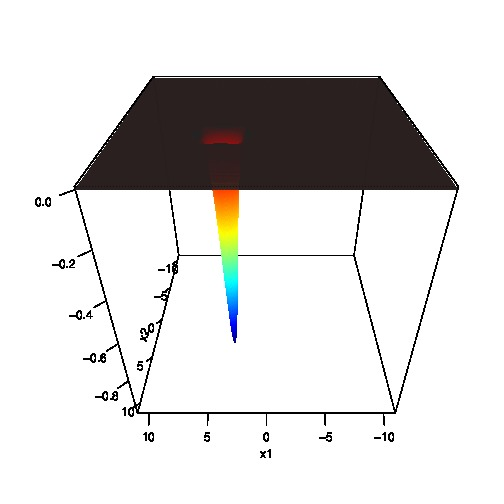
\includegraphics[width=0.49\textwidth]{./figures/easomPersp.pdf}
% 	\vspace{-0.2cm}
% 	\begin{eqnarray}
% 	f(x,y) &=& -\cos \left(x_1\right)\cos \left(x_2\right) \exp\left\{-\left[\left(x_1-\pi\right)^{2} + \left(x_2-\pi\right)^{2}\right]\right\}\\
% 	\text{Minimum}&:& f(\pi, \pi)=-1\nonumber
% 	\end{eqnarray}
% 	\end{figure}
% 	\vspace{-0.3cm}
% 	
% 	%
% 	If the Rastrigin function is an extreme example of how convergence looks in multimodal situations, then the Easom function is on the polar opposite end of that modality scale.
% 	%Further inspection of the exponential; (fundamentally they are both trigonometric in nature) in nature; (fundamentally both minima are trigonometric)
% 	Easom's single substantial minimum is similarly as sharp as the minima of Rastrigin (fundamentally they are both trigonometric in nature), however Easom's oscillations have been scaled by the exponential function so as to only emphasize the single mode present at $(\pi, \pi)$, at which, the objective value is allowed to reach its global minimum of $-1$.
% 	%, for all practical reasons,
% 	As $x$ values deviate from $\pi$, the exponential term quickly becomes vanishingly small, and thus the remainder of the search region lies practically at 0. 
% 	
% 	%
% 	%
% 	
% 	%
% 	Again to tune $\lambda$ and $w$ I consider how the EI may react to features (or lack there of in this case) of the objective function. % a search region that is so devoid of substantial features.
% 	%indicative of new minima
% 	Since Easom is so devoid of features, the objective search may only seldomly visit the single mode.
% 	% primary understand thus required to
% 	Furthermore, since the primary mode is relatively compact, it should only require a few observations from this mode to gather its general shape and minimum value.   
% 	%
% 	Thus, EI values should remain relatively consistent through out the search; the EI value only shifts slightly as the mode is quickly understood and the remainder of the unseen search space is eventually filled in.
% 	%the expectation is that 
% 	Since the EI will only experience slight shifts, this naturally implies a small value for $\lambda$.
% 	% for $\lambda$s
% 	Choosing $\lambda$ to be the lower limit from the typical range, $\lambda=0.1$, yields a lot of smoothing in the EWMA statistic.
% 	%%with a similarly sharp lone minimum among an otherwise flat surface.
% 	This heavily smoothed EWMA statistic enables the EWMA convergence chart to notice very small shifts in the underling $\E{\log\ix}$ value. 
% 	%to subject the
% 	The small value chosen for $\lambda$ implies small fluctuations in the EWMA statistic, and thus there is less opportunity to introduce small sample biases in the long run average estimates. 
% 	% 
% 	A relatively small control window is thus desirable in this case since it provides a more recent picture of the state of control, without experiencing much bias from large fluctuations.
% 	%in this case
% 	In this case $w$ was chosen to be $w=20$ iterations long.
% 	
% 	%that; seen in the previous examples the initial charts On the one hand, t
% 	The previously seen initial EWMA convergence charts, Figures (\ref{roseEWMAStart}) and (\ref{rastEWMAStart}),
% 	%
% 	%
% 	\begin{wrapfigure}{l}{0.5\textwidth}
% 	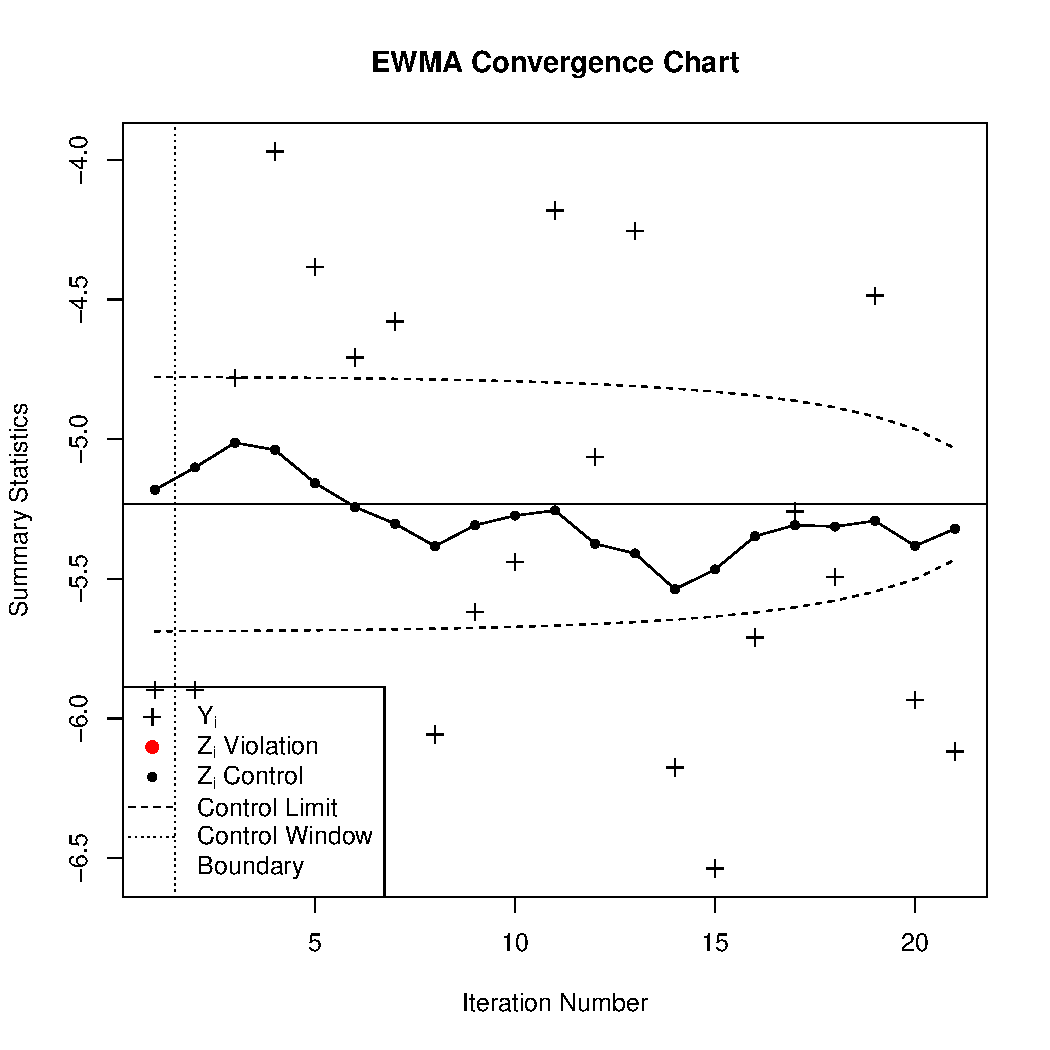
\includegraphics[width=0.245\textwidth]{./figures/ewmaConvChartEasomMedStart.pdf}
% 	\includegraphics[width=0.245\textwidth]{./figures/bestZEasomMedStart.pdf}
% 	\caption{Initial EWMA convergence chart and smallest objective function value. }
% 	\label{easomEWMAStart}
% 	$~$\\
% 	\includegraphics[width=0.245\textwidth]{./figures/ewmaConvChartEasomMedEnd.pdf}
% 	\includegraphics[width=0.245\textwidth]{./figures/bestZEasomMedEnd.pdf}
% 	\caption{Final EWMA convergence chart and smallest objective function value. }
% 	\label{easomEWMAEnd}
% 	\end{wrapfigure}
% 	%
% 	%
% 	%
% 	demonstrate a
% 	lack of convergence through a continually decreasing EWMA statistic which violates the control limits inside the control window.
% 	%the lack of{\it no}falling; out-of-control points  beyond the control window  (see Figure (\ref{easomEWMAStart})
% 	In contrast, this example experiences much more subtle EI shifts, and thus, the initial pre-converged state, seen in Figure (\ref{easomEWMAStart}), is indicated by the lack of any control limit violations.
% 	% thus far
% 	This comes from the fact that initially the objective search has not resulted in a substantial indication that the EI value has decreased enough to signal convergence.
% 	%%initial EWMA statistics violate the control limits beyond the control window.
% 	As the search continues, the lone minimum is eventually found, and the EWMA convergence chart realizes convergence as the control region shifts downward and the control limits shrink. 
% 	
% 	
% 	%\begin{itemize}
% 	%\item[\checkmark] Describe function \cite{easomCite} 
% 	%\item[\checkmark] write function down
% 	%\item[\checkmark] Pictured interval.
% 	%\item describe strategy for identifying convergence relative to characteristics of function (or expected characteristics of function).
% 	%\item thus choose $\lambda$ and $w$ appropriately.
% 	%\item discuss convergence behavior (save)
% 	%\item
% 	%\item Easom is very flat function
% 	%\item adjust lambda to, $\lambda=0.1$ to compensate.
% 	%\item adjust window size $w=20$ to pick up smaller changes inherent to smaller lambda.
% 	%\end{itemize}
% 	
% 	\clearpage
% 	%
% 	%
% 	\subsection{Lockwood Pump-And-Treat Case Study}
% 	%
% 	%
% 	
% 	%closed form
% 	The previous examples have focused on analytical functions with known minima.
% 	%
% 	This is done for the sake of developing an intuition for tuning the EWMA convergence chart parameters.
% 	%
% 	However, in most practical optimization problems it is not possible to visualize to objective function so straight forwardly, or derive theoretical minima in this way.
% 	%
% 	Thus, to demonstrate the use of the EWMA convergence chart in one such practical situation, I consider the Lockwood pump-and-treat problem presented by Matott et al. \cite{lockCite}. \\
% 	
% 	%
% 	%
% 	\begin{wrapfigure}{l}{0.5\textwidth}
% 	\vspace{0.3cm}
% 	\centering
% 	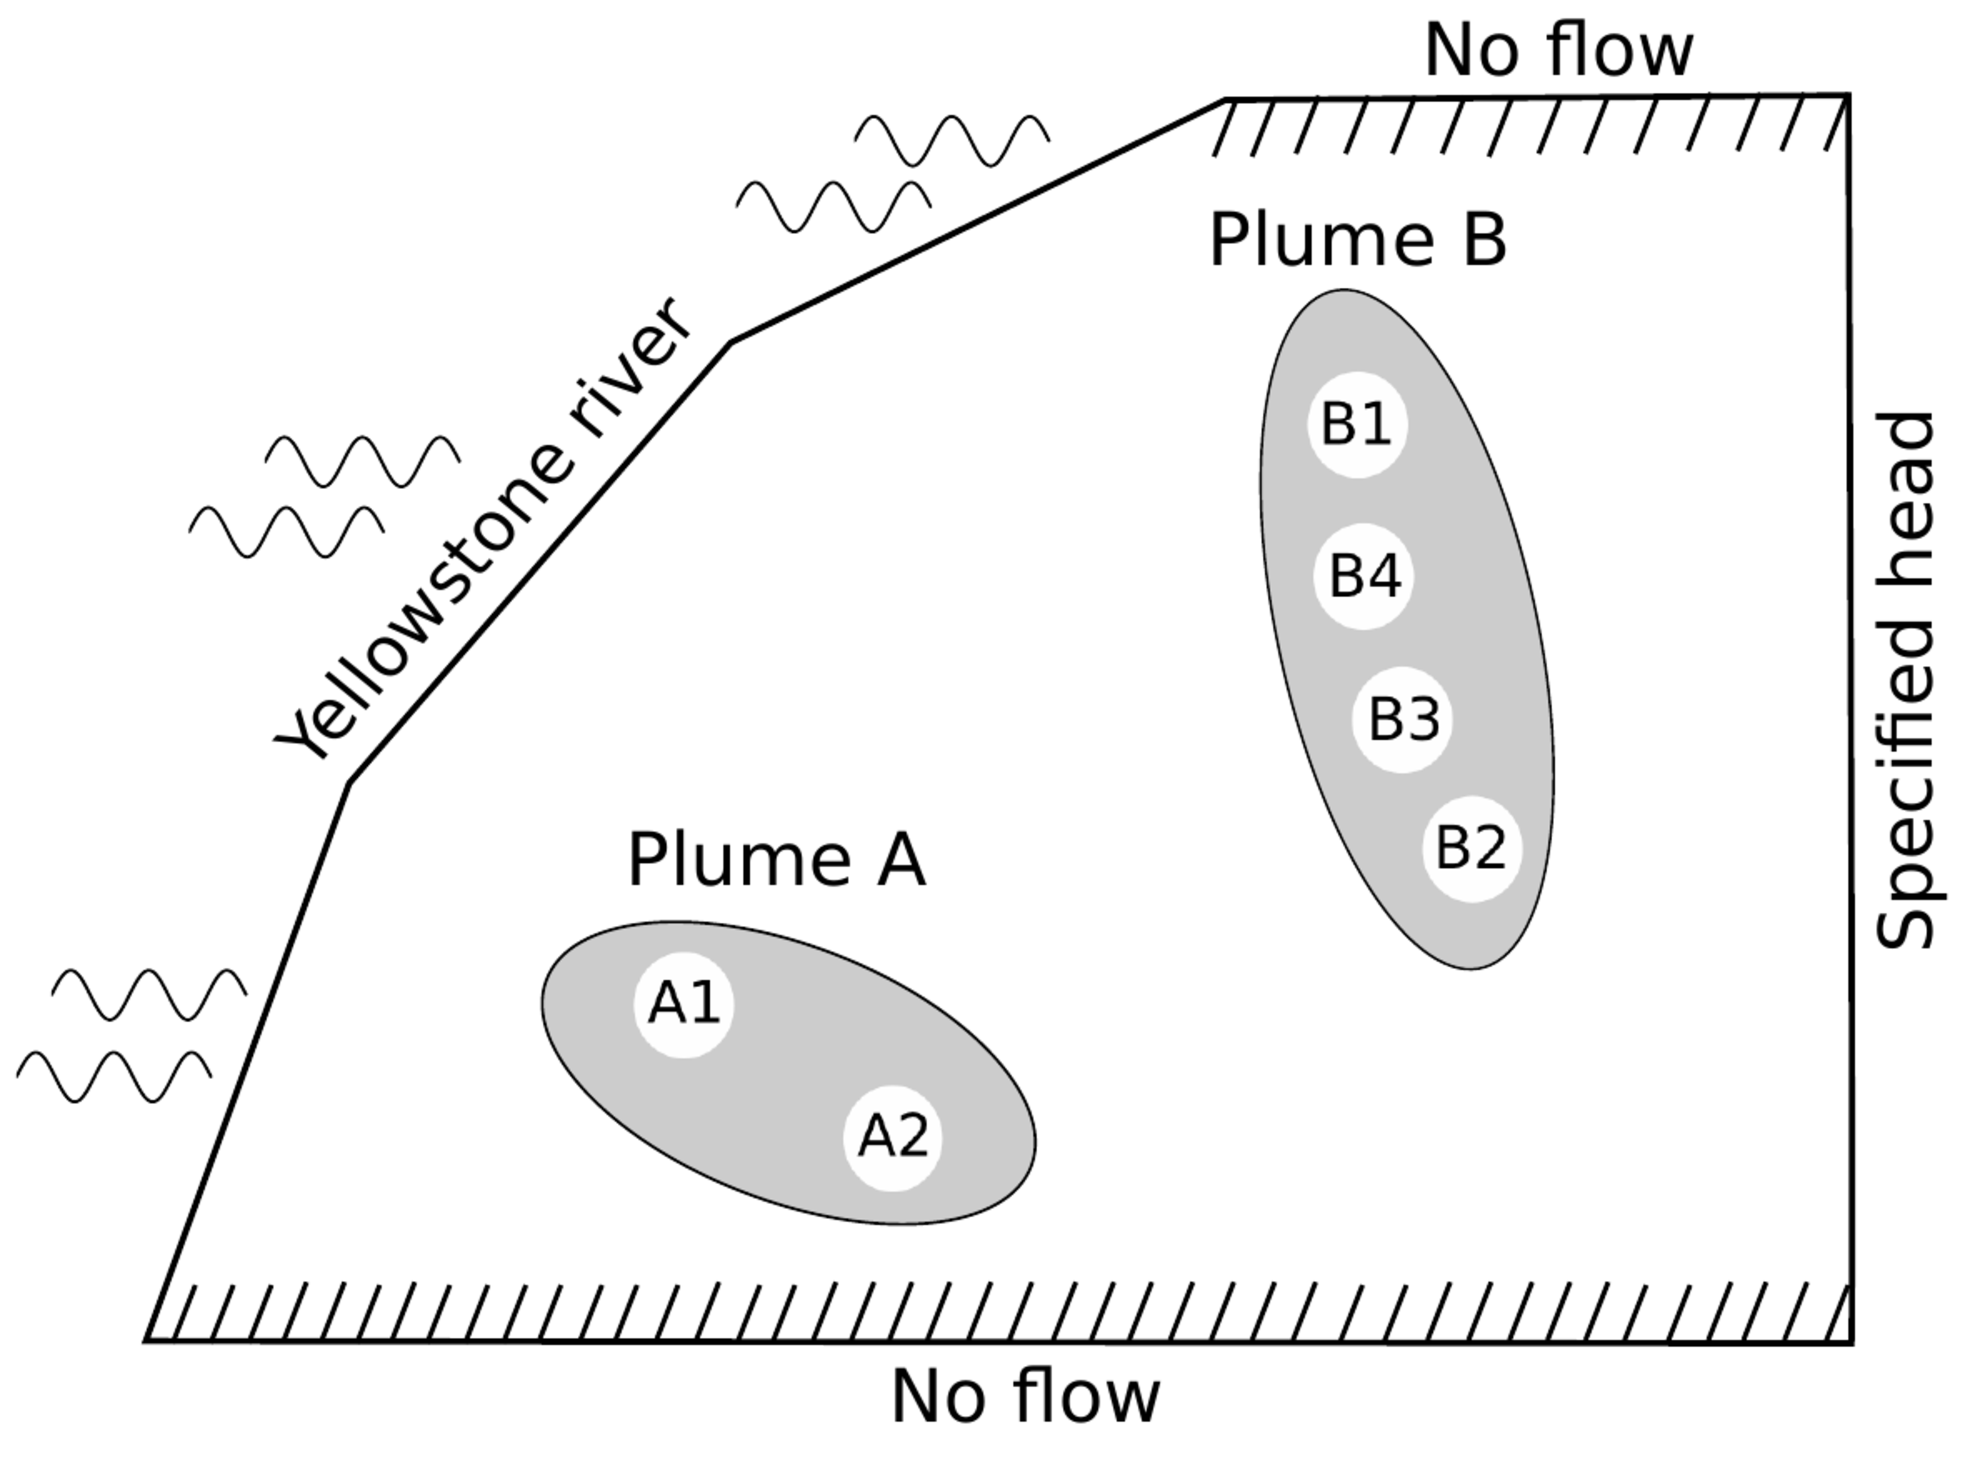
\includegraphics[width=0.5\textwidth]{./figures/Lockwood_Site_Simple.pdf}
% 	\caption{The Lockwood pumping site}
% 	\label{lockSite}
% 	\end{wrapfigure}
% 	\vspace{-0.3cm}
% 	%
% 	%
% 	
% 	%
% 	The Lockwood pump-and-treat case study considers a pumping site for chlorinated solvents located north-east of Billings, Montana, along the Yellowstone River.
% 	%
% 	The site, seen in Figure (\ref{lockSite}), contains two plumes for pumping, Plume A and Plume B, containing two and four wells respectively.
% 	%
% 	The objective is to determine the lowest cost pumping rates for each of these six wells such that contamination from the plumes does not reach the Yellowstone River.
% 	
% 	%
% 	%
% 	
% 	%, to ensure that an optimal solution never relies upon regular river contamination.a function proportional to 
% 	Thus the objective function, $f(\bm{x})$, can be expressed as the sum of the inputs, with penalties associated with contamination of the river. % by each plume, $c_A(\bm{x})$, $c_B(\bm{x})$. %$c_A(\bm{x})$ and $c_B(\bm{x})$ indicating that the  
% 	%, is the cost of operating the pumps, in USD; additionally, $f$ heavily penalizes solutions that contaminate the river.
% 	\begin{equation}
% 	f(\bm{x}) = \sum_{i=1}^6 x_i +  2\big[ c_A(\bm{x}) + c_B(\bm{x}) \big] + 20000 \big[ \oner_{c_A(\bm{x})>0} + \oner_{c_B(\bm{x})>0} \big] 
% 	\end{equation}
% 	%with simple search boundaries, \mbox{$0\le x_i\le20,000$} set for each pumping rate.
% 	Here $c_A(\bm{x})$ and $c_B(\bm{x})$ indicate the amount of contamination of the river by each plume, and $\bm{x}$ represents the pumping rate, $Q_i$, for each of the six wells.
% 	%, \mbox{$\left[x_1, ..., ~x_6\right] = \left[Q_{A1}, ~Q_{A2}, ~Q_{B1}, ~Q_{B2}, ~Q_{B3}, ~Q_{B4}\right]$}.
% 	Each $x_i$ is bounded on the relatively large interval, \mbox{$0\le x_i\le20,000$}. 
% 	%
% 	The full problem, considering all six wells, defines a six-dimensional optimization problem, but for the sake of better understanding the dynamics of the problem, it is instructive to first consider the simplified single plume problem. 
% 	%to understand the behavior of the EI criterion I first consider simplified into%with respect to $f$;
% 	The two-dimensional problem provides a nice setting for understanding the a simplified version of EI behavior, and furthermore the simplified setting develops an expectation for the EI behavior in the full \mbox{six-dimensional problem.}
% 	
% 	%\clearpage
% 	%
% 	%
% 	\subsubsection{Two-Dimensional Single Plume Problem}
% 	%
% 	%
% 	
% 	%
% 	%surrogate model of the surrogate modeling procedure.
% 	\begin{wrapfigure}{l}{0.5\textwidth}
% 	\vspace{-1.1cm}
% 	\hspace{-1cm}
% 	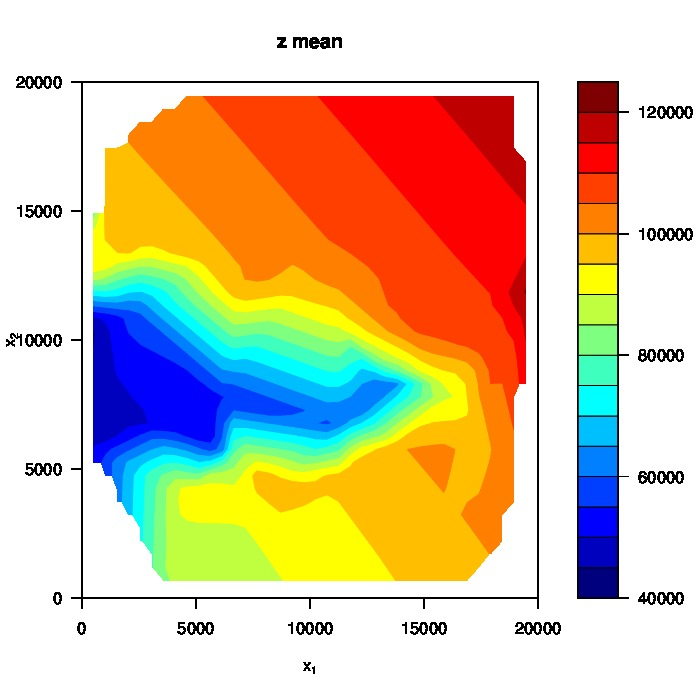
\includegraphics[width=0.5\textwidth]{./figures/gpMeanLock240000.jpg}
% 	\vspace{-0.9cm}
% 	\caption{The GP mean predictive loss surface for the two well Lockwood problem. }
% 	\label{lockGP}
% 	\end{wrapfigure}
% 	%
% 	%
% 	
% 	%and all of the wells associated
% 	The simplified search only focuses on the two wells of Plume A, and all other wells associated with Plume B, are fixed in the center of the search domain at 10,000. 
% 	% we are allowed to visualize the search space through the use of the GP surrogate model.
% 	By limiting the problem in this way, it allows for visualization of the search space via the GP surrogate model.
% 	%
% 	%In Figure (\ref{lockGP}) the GP predictive surface is seen after 400 observations of $f$.
% 	%demonstrates
% 	Figure (\ref{lockGP}) shows that much of the search space is dominated by relatively flat and consistent high loss (i.e. hot/warm colors), resulting from contamination penalties.
% 	%
% 	However, for low rates in $x_1$ and intermediate rates in $x_2$ there is a rough fissure of low cost values.
% 	%
% 	%This fissure of relatively low loss is associated with low, to intermediate, rates in $x_1$ and intermediate rates in $x_2$. 
% 	%
% 	Due to the magnitude of the contamination penalties, the walls of the Fosse seen in Figure (\ref{lockGP}) are very steep.
% 	%
% 	Furthermore, the features of the fissure floor are fairly detailed, and easy to overlook especially when compared to the relatively large search space (i.e. \mbox{$0\le x_i\le20,000$}).
% 	
% 	%\clearpage
% 	%
% 	%
% 	
% 	%
% 	Thus for determining convergence in this setting, I consider this problem to be similar to, and somewhere between, the Rosenbrock ($\lambda=0.2$) and Rastrigin ($\lambda=0.3$) test situations.
% 	%
% 	Thus $\lambda=0.25$ is an appropriate choice for the smoothing parameter.
% 	%% 	Since, $\lambda$ is in the upper region of the typical $\lambda$ range a large value for $w$ is appropriate.
% 	Again I consider the value of $\lambda$ to inform the choice of $w$.
% 	%
% 	Since $\lambda$ is in the upper region of the typical $\lambda$ range, a large value for $w$ is appropriate.
% 	%search space is  it is worth additional  not possible to get 
% 	Furthermore, since the search space is so large, the choice of a conservatively large $w$ is recommended.
% 	% 
% 	In this application $w=50$ has shown to be effective. 
% 	
% 
% 	\clearpage
% 	%
% 	%
% 	\begin{wrapfigure}{l}{0.5\textwidth}
% 	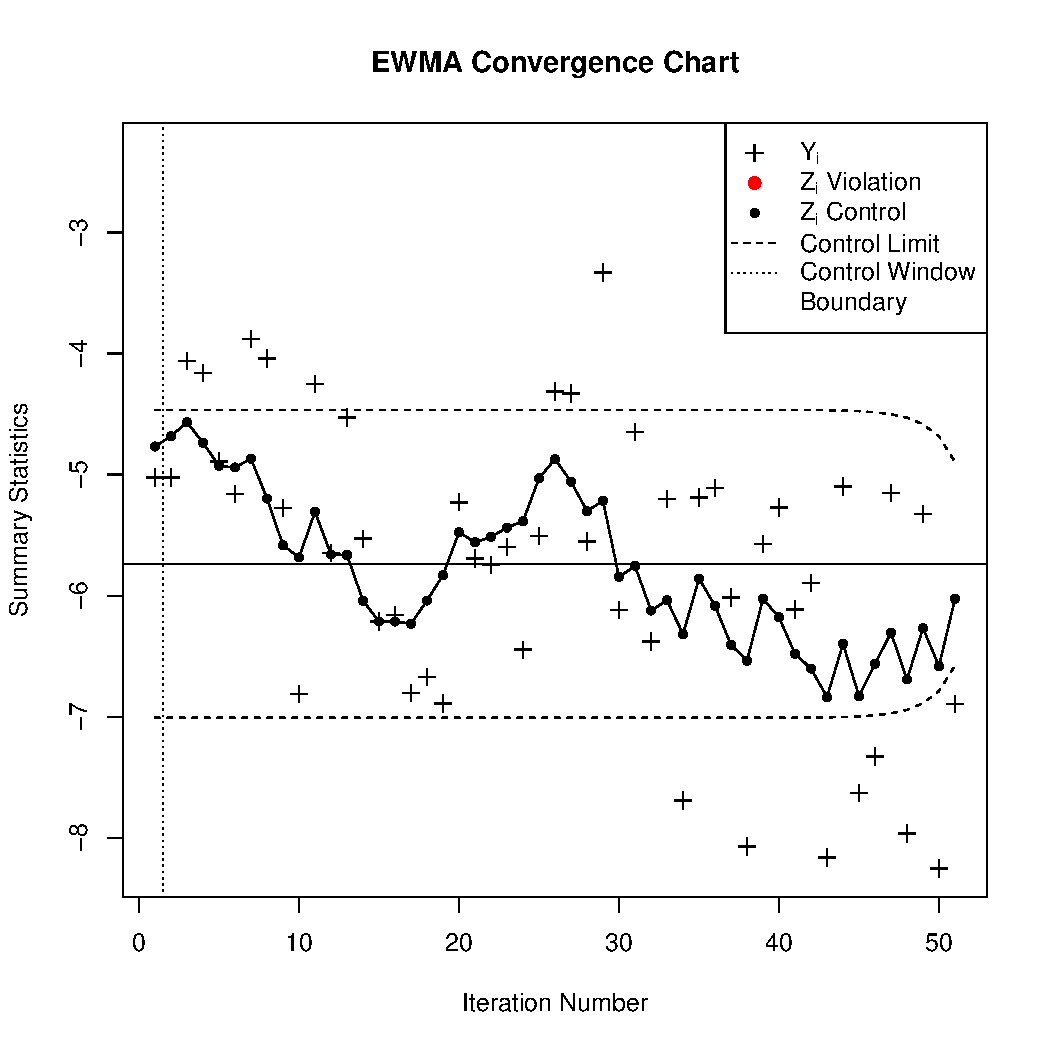
\includegraphics[width=0.245\textwidth]{./figures/ewmaConvChartLock240000Start.pdf}
% 	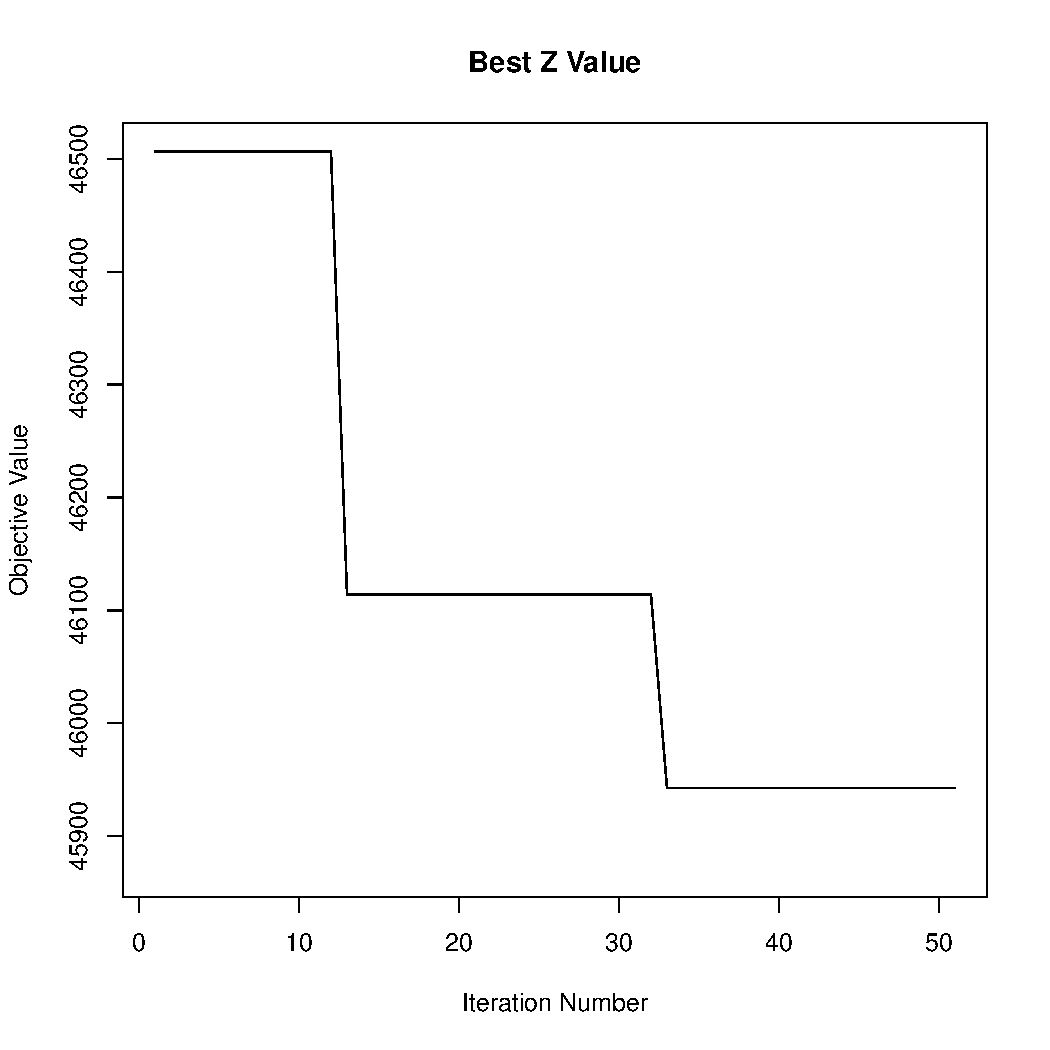
\includegraphics[width=0.245\textwidth]{./figures/bestZLock240000Start.pdf}
% 	\caption{Initial EWMA convergence chart and smallest objective function value. }
% 	\label{lock2EWMAStart}
% 	$~$\\\\
% 	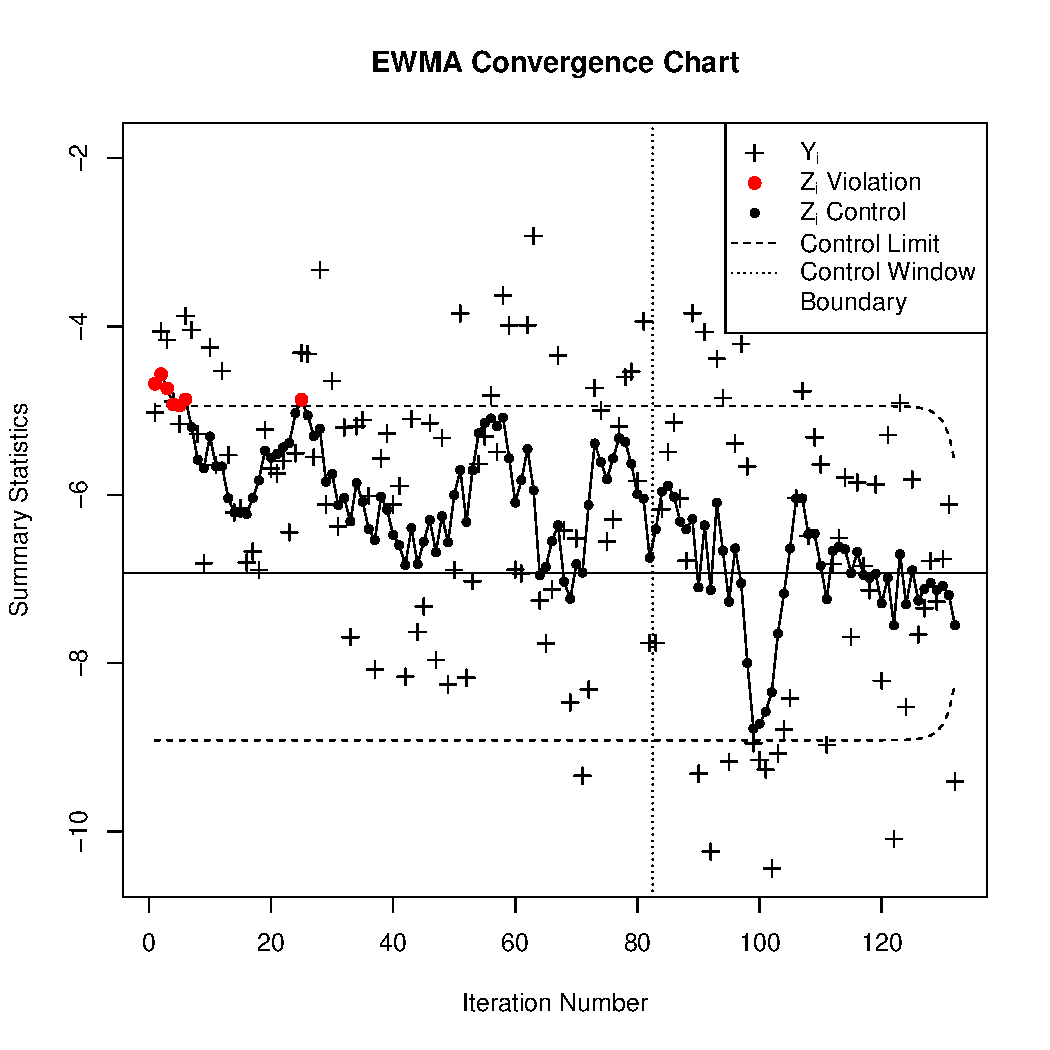
\includegraphics[width=0.245\textwidth]{./figures/ewmaConvChartLock240000End.pdf}
% 	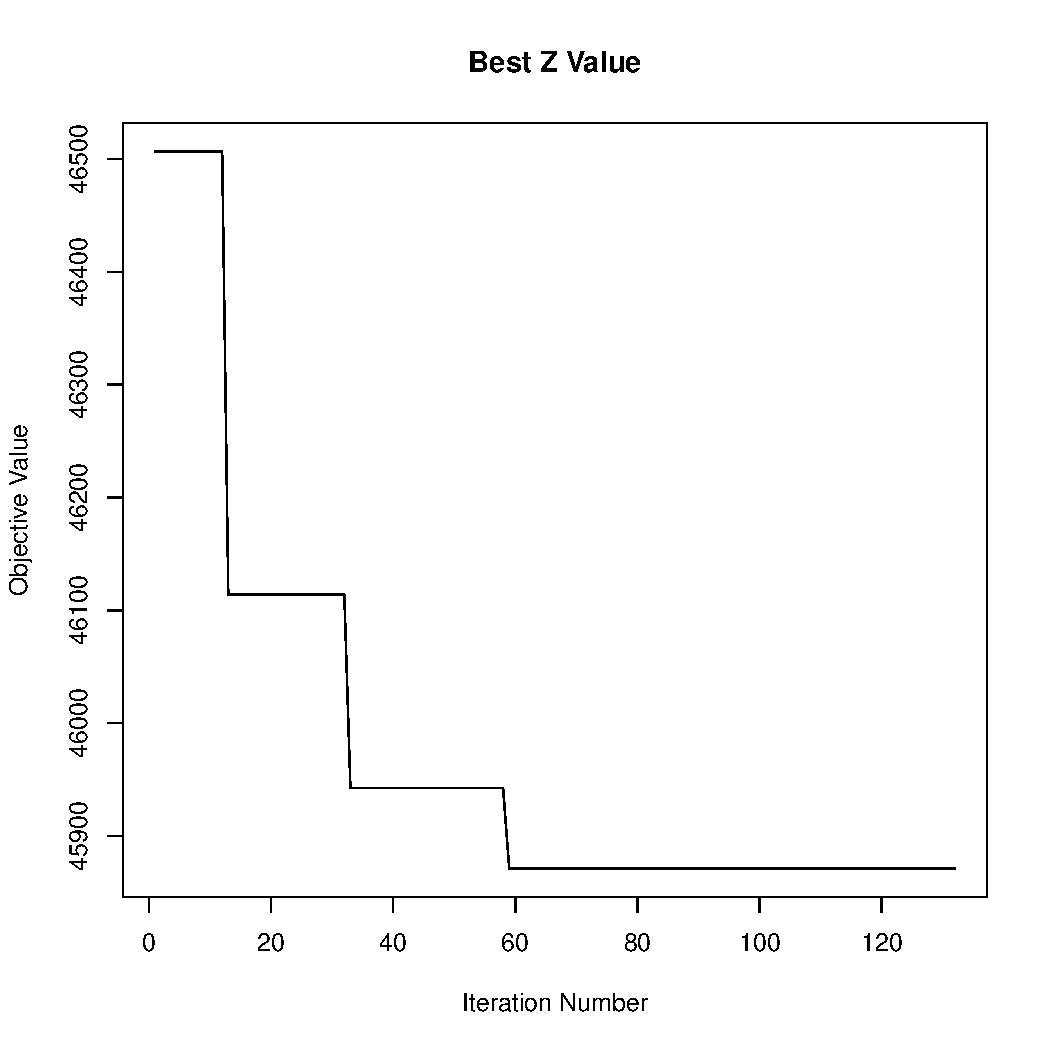
\includegraphics[width=0.245\textwidth]{./figures/bestZLock240000End.pdf}
% 	\caption{Final EWMA convergence chart and smallest objective function value. }
% 	\label{lock2EWMAEnd}
% 	\end{wrapfigure}
% 	%
% 	%
% 	
% 	%
% 	Initially the convergence chart, seen in \mbox{Figure (\ref{lock2EWMAStart}, {\it left}),} does not show any violations of the control limits.
% 	%improvement in the context of a state of
% 	Thus, \mbox{Figure (\ref{lock2EWMAStart})} does not show any signs of movement from the initial state of pre-convergence and indicates that more iterations are need to achieve convergence. 
% 	%as converged, 
% 	After about 130 iterations of optimization, violations of the upper control limit arise, indicating that the routine has explored the space \mbox{sufficiently} to announce convergence, as seen in \mbox{Figure (\ref{lock2EWMAEnd}, {\it left}).}
% 	%
% 	
% 	%
% 	%
% 	
% 	%
% 	Further analysis of the smallest observed objective values, in each of these figures, indicates that indeed this search has converged to pumping rates that are consistent with those originally reported by Matott et al. \cite{lockCite}. 
% 	%
% 	Here the smallest objective value is given for \mbox{$\bm{x} \approx \left[13,~5857,~10000,...,~10000\right]$.}    
% 
% 	\clearpage
% 	%
% 	%
% 	\subsubsection{Full Six-Dimensional Problem}
% 	%
% 	%
% 	
% 	% as well
% 	The full optimization problem not only considers the two wells of Plume A, but additionally optimizes over the four wells in Plume B.
% 	%ality
% 	By increasing the dimension of the domain, this exponentially increases the space to be explored in the objective search.
% 	%
% 	%For example, if each dimension of the domain is discretized to the integers on the set \mbox{$0\le x_i\le20,000$}, then increasing the dimension of the problem from two to six results in a $20,001^{(6-2)}\approx1.6\times10^{17}$ times larger space to search in the six dimensional problem.
% 	%is fantastically; this space is naively explored and thus
% 	Despite the large increase in the space of the objective search, recall that much of this space can be confidently ignored after the initial collection of $\bm{X}$.
% 
% 	%\clearpage
% 	%
% 	%
% 	\begin{wrapfigure}{l}{0.5\textwidth}
% 	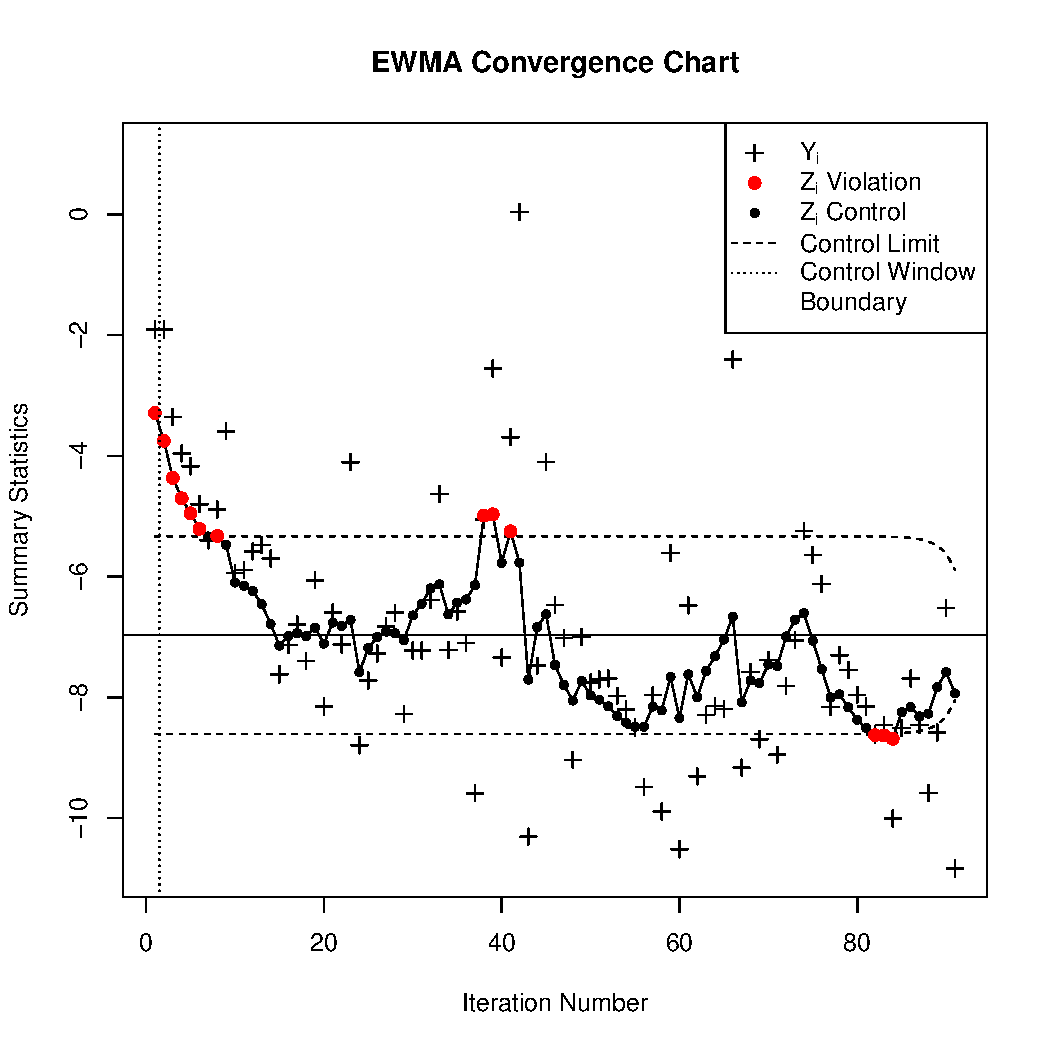
\includegraphics[width=0.245\textwidth]{./figures/ewmaConvChartLock6Three20000Start.pdf}
% 	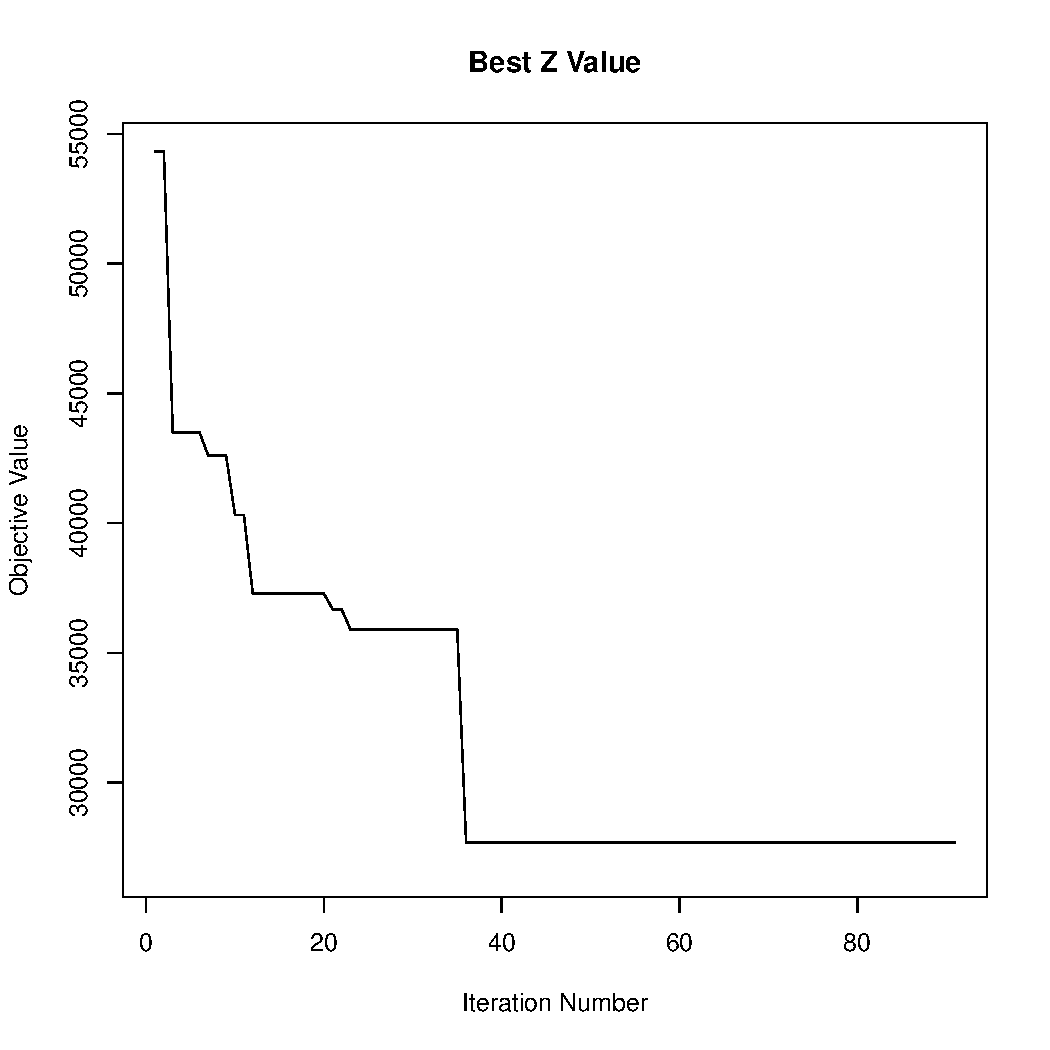
\includegraphics[width=0.245\textwidth]{./figures/bestZLock6Three20000Start.pdf}
% 	\caption{Initial EWMA convergence chart and smallest objective function value. }
% 	\label{lock6EWMAStart}
% 	$~$\\
% 	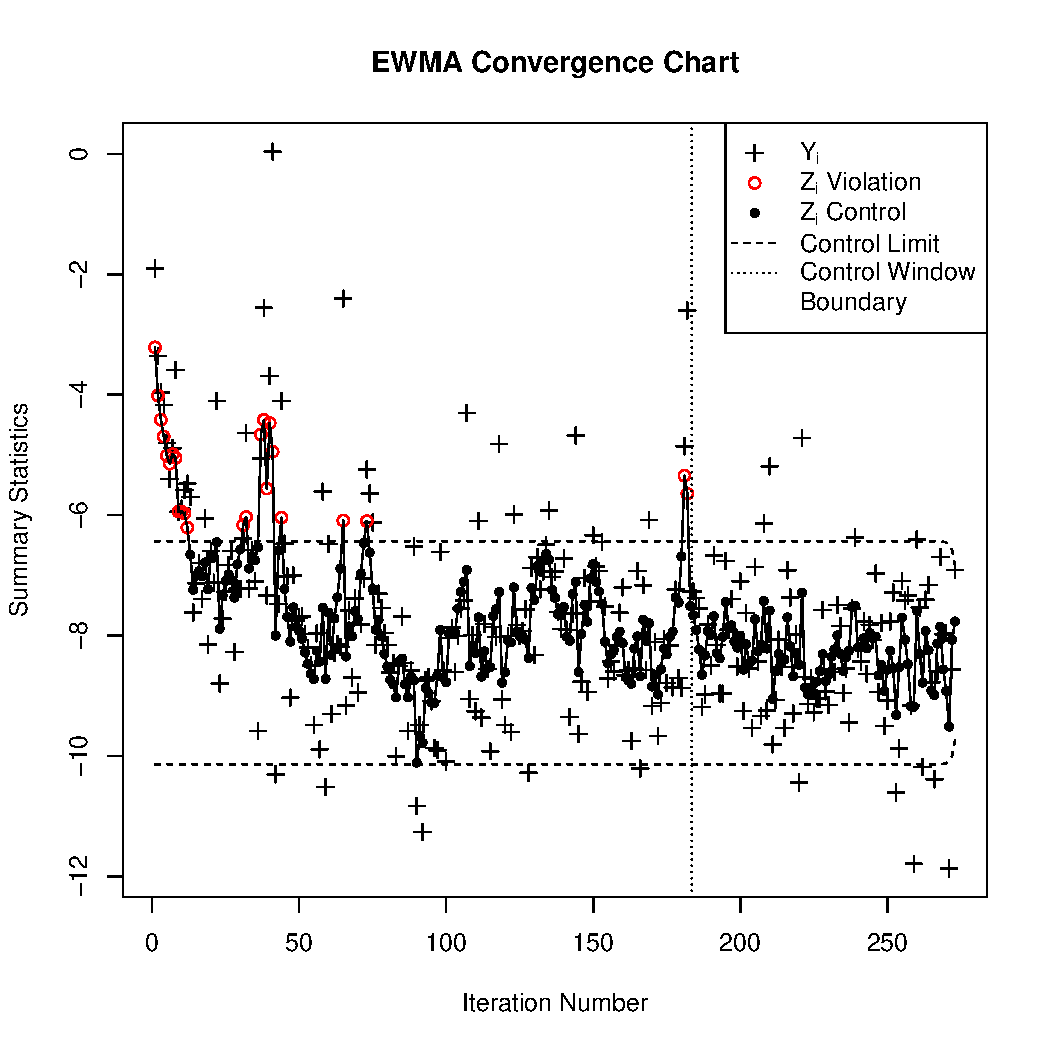
\includegraphics[width=0.245\textwidth]{./figures/ewmaConvChartLock6Three20000End.pdf}
% 	\includegraphics[width=0.245\textwidth]{./figures/bestZLock6Three20000End.pdf}
% 	\caption{Final EWMA convergence chart and smallest objective function value. }
% 	\label{lock6EWMAEnd}
% 	\end{wrapfigure}
% 	%
% 	%
% 	
% 	
% 	%that I should expect
% 	Aside from the vastly larger domain to be searched, there is no information indicating substantially different behavior from the addition of Plume B.
% 	%
% 	Thus considering the behavior of the two dimensional problem, it is reasonable to assume similar values for $\lambda$ and $w$.
% 	%I keep
% 	Here the value of $\lambda$ is kept the same as the two dimensional problem at $\lambda=0.25$, thus reflecting an intermediately lumpy objective function.
% 	%I increase the size of the control window to $w=60$.
% 	However to be conservative, considering the increased size of the domain, the size of the control window is increases to $w=90$. 
% 	
% 	%Figures (\ref{lock6EWMAStart}) and (\ref{lock6EWMAEnd})EWMA convergence
% 	Again considering the initial and final EWMA convergence chart, we see that initially in Figure (\ref{lock6EWMAStart}, {\it left}) the chart does not indicate convergence.
% 	%the right indeed best Z value
% 	%Considering the smallest objective values observed, Figure (\ref{lock6EWMAStart}, {\it right}) indicates that indeed the objective search has not discovered a substantial minimum of $f$.
% 	%Considering Figure (\ref{lock6EWMAEnd}), we observe that a %This solution % the right panel of  we see that 
% 	%In Figure (\ref{lock6EWMAEnd}, {\it right}) after about 210 iterations, the algorithm finds its lowest cost solution to be seen in 500 iterations, corresponding to an \mbox{$\bm{x} \approx \left[433,~5911,~12290,~5353,~1782,~3177\right]$}.
% 	In \mbox{Figure (\ref{lock6EWMAEnd}, {\it right})} after about 210 iterations, the algorithm finds its lowest cost solution to be seen in 500 iterations, corresponding to \mbox{$f(\bm{x})\approx26696$} at \mbox{$\bm{x} \approx \left[0,~6195,~12988,~3160,~1190,~3163\right]$}.
% 	%
% 	%This turns out to provide the lowest objective value to be discovered in 500 iterations of the algorithm.
% 	%we see
% 	Considering Figure (\ref{lock6EWMAEnd}, {\it left}), the EWMA convergence chart identifies this convergence after only about 270 iterations.
% 	%2.016075e-01 6.195005e+03 1.298804e+04 3.160273e+03 1.189587e+03 3.163334e+03
% 	%432.885  5910.821 12289.646  5352.652  1782.080  3177.451
% 	%\mbox{$\bm{x} \approx \left[3,~7093,~13791,~4471,~6158,~111\right]$} $f(\bm{x}) \approx 31627$
% 
% 	
% % \clearpage
% \doublespacing
% % 	
% % 	
% \section{Conclusion}
% % 	
% % 	
% 
% %
% % Identifying convergence in numerical optimization can be difficult due to the subjective nature of convergence. 
% % to give convergence a more objective definition.
% Through the use of SPC ideas the EWMA convergence chart provides an objective definition of convergence. 
% %in this papeheredemonstrates its ability to
% If properly tuned, the examples provided demonstrate how the  EWMA convergence chart may accurately, and efficiently, identify convergence in the context of GP surrogate model optimization.
% 
% %
% %
% 
% %in optimization It is worth mentioning here that a
% As for any optimization algorithm, the solution found may only be considered as good as the algorithms specific characterization of $f$.
% %
% Thus a poorly tuned surrogate modeling strategy may never optimize $f$ to its fullest extent.
% %
% In cases of poorly tuned optimization algorithms, the EWMA convergence chart presented here may only identify convergence with respect to the quality of the particular surrogate modeling strategy used.
% %discovery 
% Thus for poorly tuned surrogate modeling strategies the EWMA convergence chart may only identify that the algorithm has reached a point of diminishing returns; for correctly tuned surrogate modeling strategies this point corresponds with the realization of an optimal solution.
% %at which the EWMA convergence chart claims convergence corresponds with the discovery of an optimal solution.
% %
% In either poor or correct tuning, the EWMA convergence chart identifies the moment at which it is beneficial to stop the routine to reflect upon the results.
% %
% %That is to say that when the either way stopping optimization  is useful to re-tune the algorithm, or enjoy the spoils of a succfull optimization algorithm.  
% 
% %
% %
% 
% % all of the tested applications.
% %provided my study with an effective outcome in all of the applications shown here 
% %I have outlined a strategy that has shown to be effective, in my applications, for tuning the parameters of the EWMA convergence chart.
% The strategy shown here for tuning $\lambda$ and $w$ demonstrates an empirically effective approach for tuning the EWMA convergence chart parameters. 
% %
% This approach is mainly useful due to its simplicity, although other more pointed methods may surely calculate more effective values.
% %
% Box et al. \cite{boxBook} demonstrates quantitative methods for choosing $\hat\lambda$ so as to minimize the sum of squared deviation ($S_\lambda$), however this method was not considered here because it introduces additional optimization problems (albeit univariate and apparently simple).
% %
% The methods proposed by Box et al. may be extended to the EWMA convergence chart by considering some initial set of optimization iterations and considering the following bivariate optimization problem \mbox{$\left\{\hat\lambda, \hat w \right\} = \argmin_{\lambda, w} S(\lambda, w)$.} 
% 
% % \clearpage
% %
% %
% 
% %, observed in the first few iterations of the algorithm,
% The heuristics of the EWMA convergence chart were specifically chosen based on the behavior of EI criterion, however occasionally the initial optimistically high values of the EI criterion can produce situations that are susceptible to false convergence.
% %
% Since the first few iterations will always produce the first EI values to exit the control window, if these values are very large they may not be adequately tamed by the exponentially decreasing weights, as intended. % weights on these values may fail to taim this optimism.
% %
% Thus a conservative strategy for \mbox{combating} this initial optimism could involve removing the first few iterations of optimization from the analysis of the EWMA convergence chart.
% %
% This removal may be justified based on the notion that these observations are outliers that do not represent the initial pre-convergence state of control that is implicitly assumed here. 


%
%
\clearpage
\newgeometry{ margin=1in, top=0.6in, footskip=0.4in }
\singlespacing
\bibliographystyle{plain}
\bibliography{./spcCite}
%
%

\end{document}
































